\documentclass[MTech]{iitmdiss}

\usepackage{times}
\usepackage{epsf}
\usepackage{threeparttable}
\usepackage{setspace}
\usepackage{amsmath}
\usepackage{gensymb}
\usepackage{amsthm}
\usepackage{txfonts,pxfonts,amsfonts}
\usepackage{epsfig}
\usepackage{caption}
\usepackage{subcaption}
\usepackage{graphicx}
% \usepackage[square,numbers,sort]{natbib}
\usepackage[square]{natbib}
\usepackage[hidelinks]{hyperref} % hyperlinks for references.
\usepackage{algorithm}
\usepackage{placeins}
\usepackage{algpseudocode}

\makeatletter
\def\BState{\State\hskip-\ALG@thistlm}
\makeatother
%\include{commands}
\newcommand{\plt}{thesis_plots}
% Strut macros for skipping spaces above and below text in tables. 
\def\abovestrut#1{\rule[0in]{0in}{#1}\ignorespaces}
\def\belowstrut#1{\rule[-#1]{0in}{#1}\ignorespaces}

\def\abovespace{\abovestrut{0.20in }}
\def\aroundspace{\abovestrut{0.20in}\belowstrut{0.10in}}
\def\belowspace{\belowstrut{0.10in}}
%%%%%%%%%%%%%%%%%%%%%%%%%


\def\thesistitle{Motivic analysis of neuronal responses to visual stimuli}
\def\thesisauthor{Athul Vijayan}


\begin{document}
\bibliographystyle{iitm}
%%%%%%%%%%%%%%%%%%%%%%%%%%%%%%%%%%%%%%%%%%%%%%%%%%%%%%%%%%%%%%%%%%%%%% 
% Title page

\title{\thesistitle}

\author{\thesisauthor}

\date{April 2016}
\department{Engineering Design}

%\nocite{*}
\begin{singlespace}
\maketitle 
\end{singlespace} 



%%%%%%%%%%%%%%%%%%%%%%%%%%%%%%%%%%%%%%%%%%%%%%%%%%%%%%%%%%%%%%%%%%%%%%
% Certificate
\certificate

\vspace*{0.5in}

\noindent This is to certify that the thesis entitled {\bf {\thesistitle}}, 
submitted by {\bf {\thesisauthor}}, to the Indian Institute of Technology, 
Madras, for the award of the degree of {\bf Master of Technology}, 
is a bona fide record of the research work carried out by him under my
supervision. The contents of this thesis, in full or in parts, have not been
submitted to any other Institute or University for the award of any degree or
diploma.

\vspace*{1.4in}
\hspace*{-0.25in}
\begin{minipage}{.5\textwidth}
\begin{singlespace}
\noindent {\bf Dr.~Hema~A.~Murthy } \\
\noindent Research Guide \\ 
\noindent Professor \\
\noindent Dept. of Computer Science\\
\noindent IIT-Madras, 600 036 \\
\end{singlespace}
\vspace*{0.20in}
\noindent Place: Chennai\\ 
Date:
\end{minipage}%
\begin{minipage}{.5\textwidth}
\begin{singlespace}
\noindent {\bf Dr.~Srikanth~Vedantam } \\
\noindent Research Guide \\ 
\noindent Professor \\
\noindent Dept. of Engineering Design \\
\noindent IIT-Madras, 600 036 \\
\end{singlespace}
\vspace*{0.20in}
\noindent Place: Chennai\\ 
Date:
\end{minipage}%
%%%%%%%%%%%%%%%%%%%%%%%%%%%%%%%%%%%%%%%%%%%%%%%%%%%%%%%%%%%%%%%%%%%%%%
% Acknowledgements
\acknowledgements

Foremost, I would like to express my sincere gratitude to my guide Dr.~Hema~A.~Murthy for the continuous support in the work, for her patience, motivation, enthusiasm, and immense knowledge in the field. I thank my committee members, especially Prof Srikanth Vedantam, who gave the liberty to pursue a project of my choice.

I would like to thank Dr. Mriganka Sur, MIT for inspiring me to the field of Neuroscience and for the opportunity I received to work in collaboration with Sur's lab, MIT. I thank Rajeev Rikhye for sharing experimental data and his valuable guidelines.


I am thankful to DON Lab family for a wonderful time and great support. I thank my parents for supporting throughout my life. I would like to thank Midhila Mohan for keeping me motivated in pursuing my dreams.

I would like to thank everyone I met in my life.

%%%%%%%%%%%%%%%%%%%%%%%%%%%%%%%%%%%%%%%%%%%%%%%%%%%%%%%%%%%%%%%%%%%%%%
% Abstract
\abstract
\noindent KEYWORDS: \hspace*{0.5em} \parbox[t]{4.4in}{Motif, Neuronal data analysis, Neuronal correlations, Orientation and directional selectivity, Primary visual cortex, RLCS, ACFGram, Reliability of neurons}
\vspace*{24pt}

Neurons in primary visual cortex (V1) are known to be orientation and direction selective. Even with the understanding of the characteristics of neurons, a reliable information encoding mechanism in V1 is not well understood. Individual neuronal responses are known to be less reliable. Reliability is believed to exist in population responses rather than an individual neuron. Inter-neuronal correlations are great way to study information coding in a population of neurons. 

Motifs are well studied in the context of music. Motifs in Carnatic music is based on the concept of \textit{raga}. Melodic motifs are signature phrases that give \textit{raga} its identity [\cite{ishwar2013motif}]. We define motif in neuronal responses as subsequence of a response signal having significant length and repeats itself in other neuronal responses. 

In this study, we analyses neuronal responses for the existence of motifs. The best motifs are then extracted with a signal matching algorithm - RLCS. The study showed presence of motifs across trial and across neurons in a mice. Presence of repeating subsequences with significant length provides more inferences on individual neuron reliability and inter-neuronal correlations. A new correlation measure for studying the Inter-neuronal similarity is proposed.


\pagebreak
%%%%%%%%%%%%%%%%%%%%%%%%%%%%%%%%%%%%%%%%%%%%%%%%%%%%%%%%%%%%%%%%%%%%%%
% Table of contents etc.

\begin{singlespace}
\tableofcontents
\thispagestyle{empty}

\listoftables
\addcontentsline{toc}{chapter}{LIST OF TABLES}
\listoffigures
\addcontentsline{toc}{chapter}{LIST OF FIGURES}
\end{singlespace}


%%%%%%%%%%%%%%%%%%%%%%%%%%%%%%%%%%%%%%%%%%%%%%%%%%%%%%%%%%%%%%%%%%%%%%
% Abbreviations
\abbreviations
 
\noindent 
\begin{tabbing}
xxxxxxxxxxx \= xxxxxxxxxxxxxxxxxxxxxxxxxxxxxxxxxxxxxxxxxxxxxxxx \kill
\textbf{RLCS}   \> Rough Longest Common Subsequence \\
\textbf{LCSS}   \> Longest Common Segment Set \\
\textbf{ANN}   \> Artificial Neural Networks \\
\textbf{OSI}   \> Orientation Selectivity Index \\
\textbf{DSI}   \> Direction Selectivity Index \\
\textbf{PCA}   \> Principal Component Analysis \\
\textbf{ACF}   \> Auto-Correlation Function \\
\textbf{V1}  \> Primary Visual Cortex

\end{tabbing}

\pagebreak

%%%%%%%%%%%%%%%%%%%%%%%%%%%%%%%%%%%%%%%%%%%%%%%%%%%%%%%%%%%%%%%%%%%%%%
%Notation

\chapter*{\centerline{NOTATION}}
\addcontentsline{toc}{chapter}{NOTATION}

\begin{singlespace}
\begin{tabbing}
xxxxxxxxxxx \= xxxxxxxxxxxxxxxxxxxxxxxxxxxxxxxxxxxxxxxxxxxxxxxx \kill
\textbf{$\rho(a, b)$}  \> Pearson correlation between $a$ and $b$\\
\textbf{$R(\theta_k)$}  \> The average response of a neuron to orientation angle angle $\theta_k$.\\
\textbf{$R_A$}  \> Reliability measure of a neuron to visual stimuli $A$\\
\textbf{$X$}  \> Discrete signal $(x1, x2...xm)$\\
\textbf{$X_i$}  \> Discrete signal $(x1, x2...xi)$\\
\textbf{$\delta$}  \> Constant penalty for sample mismatch\\
\textbf{$\tau_{dist}$}  \> Distance threshold below which samples are considered as a match.

\end{tabbing}
\end{singlespace}
 
 \pagebreak
 \clearpage

\pagenumbering{arabic}


%%%%%%%%%%%%%%%%%%%%%%%%%%%%%%%%%%%%%%%%%%%%%%%%%%%%%%%%%%%%%%%%%%%%%%
\chapter{Introduction}   % 2 pages
\label{chap:intro}
Neuroscience in modern world is an interdisciplinary science collaborating with many other fields like cognitive science, computer science, linguistics, medicine and philosophy. To understand a sophisticated system as the brain requires an interdisciplinary approach. Advances in modern imaging tools and machine learning models like Artificial Neural Network (ANN) enables us to study how the brain performs complex functions like vision. Understanding of the brain will help us design systems that are as powerful as the brain itself. Artificial Neural Networks (ANN) are remarkable machine learning models inspired from the functioning of brain. 

Machine learning and signal processing work harmoniously to find patterns and their meaningful inferences from experimental data. The ability of algorithms to learn like the brain is intriguing. In this regard, a better understanding of the brain will help us create complex Artificial Intelligence systems.

Visual perception is a complex function performed by the brain. Visual pathway in brain starts from retina in the eye. Rods and cons are photo-receptor cells in the eye that are connected to the brain through neurons. Understanding information coding in brain will provide insights on neural circuitry in the brain. A neuron is reliable if it produces similar response every time a stimuli is presented to it. If we can perceive a same input correctly each time, there must be some form of information coding. Individual neuronal responses are not reliable due to intrinsic noise. It is believed that primary visual cortex (V1) codes information in population with inter-neuronal correlations.


Motifs are well studied in the context of music. Motifs in Carnatic music is based on the concept of \textit{raga}. Melodic motifs are signature phrases that give \textit{raga} its identity [\cite{ishwar2013motif}]. In Genetics, motif is a sequence pattern of nucleotides in a longer DNA sequence. In neuronal responses we define motif as subsequence of a response signal having significant length and repeats itself in other neuronal responses.

This work use signal processing and machine learning approaches to recognize patterns in responses of neurons in primary visual cortex to various visual stimuli. An understanding of the characteristics of neurons in V1 are given, and further the properties are quantified from experimental data. This work study the presence of motifs in neuronal signals. Inter-trial motifs are analyses in search of reliable subsequences in an individual neuron. Inter-neuronal motifs are used in analyzing the correlation between neurons. A better correlation measure is proposed to determine similarity between two neurons. Neuronal signals from two different mice were searched for motifs. These motifs were found to be small in length, yet their presence could be due to similar activation mechanism of neurons.

%%%%%%%%%%%%%%%%%%%%%%%%%%%%%%%%%%%%%%%%%%%%%%%%%%%%%%%%%%%%%%%%%%%%%%
\chapter{Background and Previous work}    %8  pages
\label{chap:lit}
Signal processing and machine learning methods are great tools to bring out valuable inferences from data. The conclusions we draw from statistical methods will have meaning only in the context of the problem. To analyze and draw conclusions from neuronal data, we need to have a good understanding of the background. This chapter provides background in basic Neuroscience and previous works in the similar problem.
\section{Visual pathway in brain} % (fold)
\label{sec:visual_pathway_in_brain}
Brain is the most sophisticated organ nature has devised. The brain is mainly made up of orderly arrays of cells called neurons (also called nerve cells). Neurons are electrically excitable cells which process information through electrical and chemical processes. Neurons are also information carriers that connect the whole body to the brain. Visual perception is a computationally complex function yet the brain performs it very efficiently. There are over 100 million photo-receptors in a human retina, but only around 1 million axons carry information to the brain [\cite{bear2007neuroscience}]. Understanding how the brain represents and processes visual information can help us create artificially intelligent machines with vision abilities.

This section describes functioning of neurons and background on visual pathway of brain.
\subsection{Neurons} % (fold)
\label{sub:neurons}
A neuron consists of three parts - soma, dendrites and axons. Soma is the cell body of neuron housing many organelles including Nissl granules and Nucleus. Axon is the signal transmitting nerve fiber that emerges from the soma. Dendrites are branched fibers that receive information from other nerve cells. The axon can be anywhere from less than a millimeter to a meter or more in length; the dendrites are mostly in the millimeter range. Near the point where it ends, an axon usually splits into many branches, whose terminal parts come very close to but do not quite touch the cell bodies or dendrites of other nerve cells. At these regions, called synapses, information is conveyed from one nerve cell, the presynaptic cell, to the next, the postsynaptic cell [\cite{hubel1995eye}].
% \begin{figure}[h]
% \centering
%   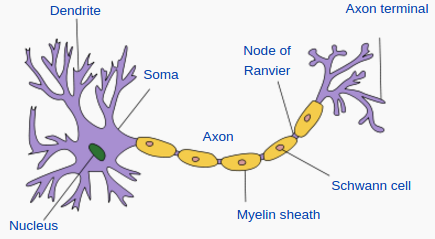
\includegraphics[width=.6\linewidth]{\plt/neuron_ana.png}
%   \caption{Anatomy of a neuron. Attribution: Quasar Jarosz at English Wikipedia}
%   \label{fig:neuron_ana}
% \end{figure}
The function of a nerve cell is to take in information from the cells that feed into it, process that information, and to deliver the integrated information to other cells. The information is usually conveyed in the form of brief events called nerve impulses. The nerve cell is bathed in and contains salt water. Because most of the salt molecules are ionized, the fluids both inside and outside the cell will contain chloride, potassium, sodium, and calcium ions (Cl , $\text{K}^+$, $\text{Na}^+$ and $\text{Ca}^{2+}$).
In the resting state, the inside and outside of the cell differ in electrical potential by 0.07 volts. The signals that the nerve conveys consist of transient changes in this resting potential, which travel along the fiber from the cell body to the axon endings. During an impulse, a large number of sodium pores in a short length of the nerve fiber suddenly open, so that briefly the sodium ions dominate and that part of the nerve suddenly becomes negative outside, relative to inside. The sodium pores then re-close, and meanwhile even more potassium pores have opened than are open in the resting state. Both events - the sodium pores re-closing and additional potassium pores opening - lead to the rapid restoration of the resting state with positive potential outside . The whole sequence lasts about one-thousandth of a second. [\cite{hubel1995eye}]

Neuronal responses are quantified by measuring the number of spikes per second - called spike rate. In this work, we measure $\text{Ca}^{2+}$ concentration as the response of neuron. As the spikes are caused by the ion concentration changes, $\text{Ca}^{2+}$ ion concentration is a good proxy for spike rate. The Vogelstein deconvolution algorithm [\cite{vogelstein2010fast}] extracts the spike train of each neuron from a raw fluorescence movie. We use the inferred spike rate from the Vogelstein deconvolution algorithm as the neuron's response.

\subsection{Visual pathway} % (fold)
\label{sub:visual_pathway}
The brain performs the enormous task of translating light that falls on retina into a meaningful visual scene. The visual pathway starts with eye, of which most important part is the retina. Retina contains light receptors called rods and cones. Rods are far more numerous than cones and are responsible for our vision in dim light but do not respond to bright light. Cones do not respond to dim light but are responsible for our ability to see fine detail and for our color vision. The layer of nerve cells at the back of the retina consist of retinal ganglion cells which connect eye to the brain through optic nerve.

Receptive field refers to the specific receptors that input information into a given cell in the nervous system. In visual pathway, it refers to a region on the retina from which information goes to a particular neuron. Receptive fields of adjacent neurons are usually  overlapping. As we go into higher levels of visual pathway, the receptive field gets complicated.

The optical nerve reaches lateral geniculate cells before it join the primary visual cortex in the brain. About half the fibers coming from a particular eye cross to the side of the brain opposite the eye of origin, and half stay on the same side. Lateral geniculate cells receive fibers from the cerebral cortex also, which plays some role in attention. The primary visual cortex (V1) is a plate of cells 2 millimeters thick, with a surface area of a few square inches. V1 contains three different kinds of cells - simple cells, complex cells and orientation insensitive cells. Neurons in V1 are orientation selective cells which can represent visual information in terms of edges as visual features. [\cite{hubel1995eye}]

Neurons in V1 are selective to orientation and direction of a visually contrasting pattern in the receptive field. The orientation is the angle to which the patterns is aligned, direction is the angle to which the pattern is moving in the next frame. Figure~\ref{fig:ori_resp} shows the behavior of orientation selective neurons. They have a preferred orientation to which they produce an optimum response. As the orientation deviates from preferred orientation, the response reduces exponentially. 
\begin{figure}[h]
\centering
  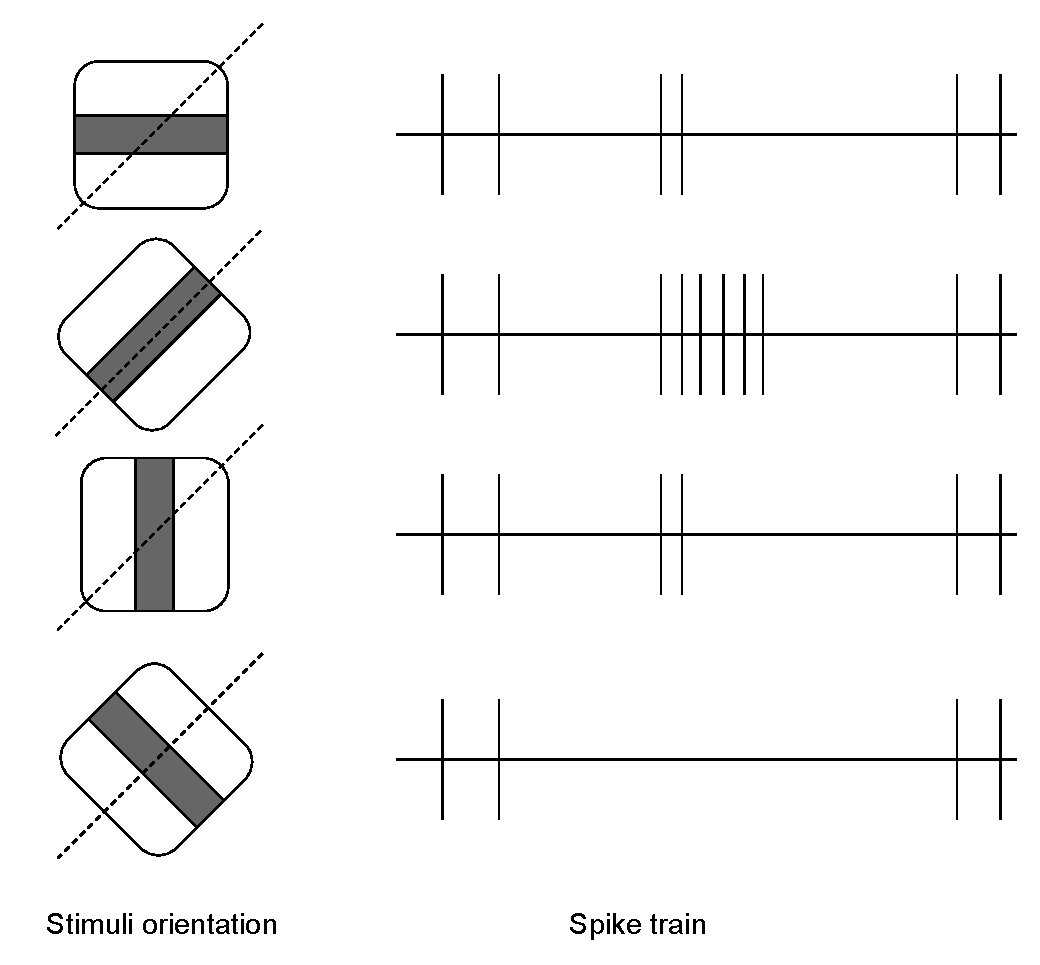
\includegraphics[width=.6\linewidth]{\plt/ori_selectivity.pdf}
  \caption{Spike train response of an orientation selective neuron. The cell has a preferred orientation which is shown by dashed line. Response reduce exponentially when the stimuli orientation deviates from preferred orientation}
  \label{fig:ori_resp}
\end{figure}
Within orientation selective cells, there are two kinds of cells - simple and complex cells. Consider moving the oriented stimuli perpendicular to the angle of orientation. Among the two perpendicular directions, some neurons respond to one perpendicular direction more than the other. These cells are called complex cells. Neurons which respond similar to both directions of motion is called simple cells. The Figure explains the directional sensitivity of simple and complex cells.
\begin{figure}[h]
  \begin{subfigure}[b]{0.5\textwidth}
    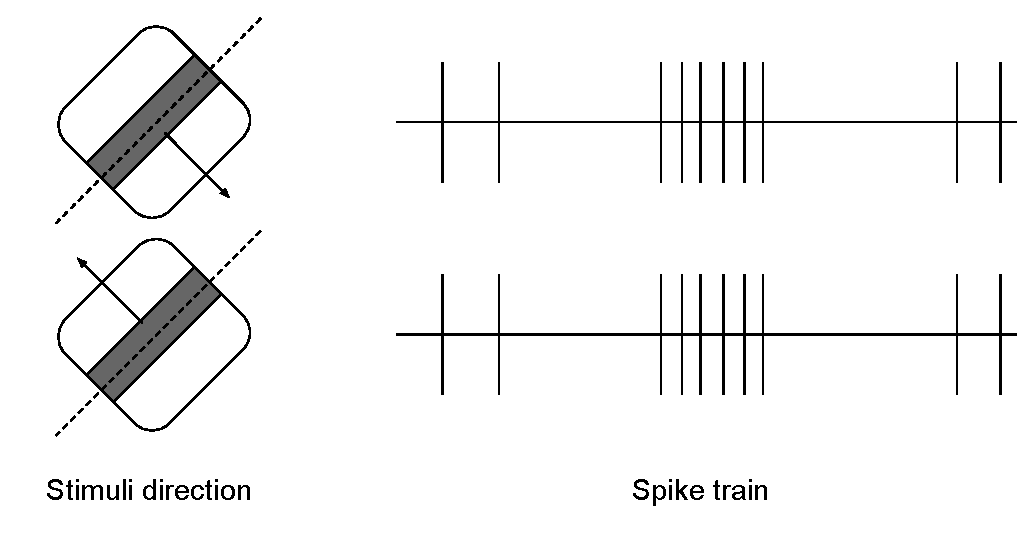
\includegraphics[width=\linewidth]{\plt/dir_simple.pdf}
    \caption{Response of simple cell to direction}
    \label{fig:ori_simple}
  \end{subfigure}%
  \begin{subfigure}[b]{0.5\textwidth}
    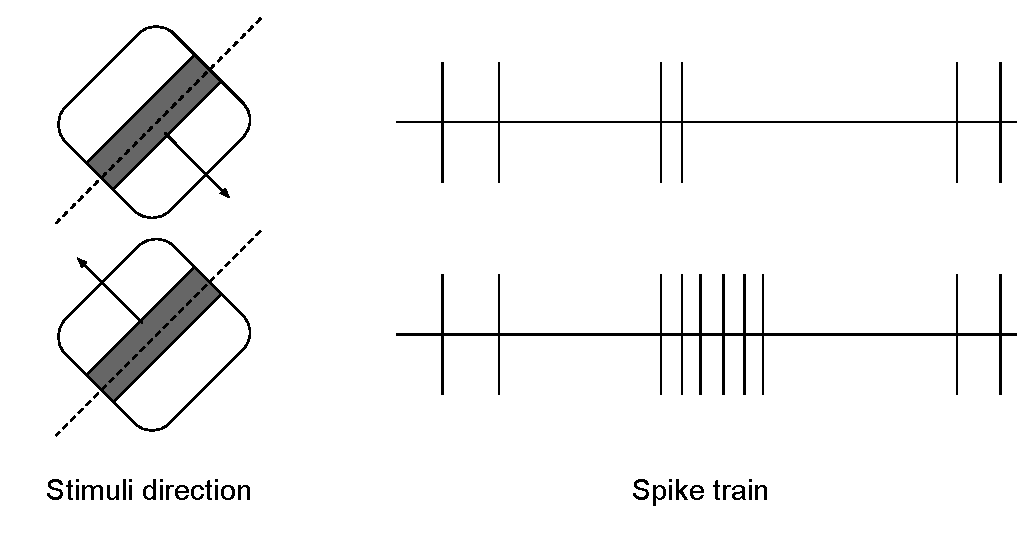
\includegraphics[width=\linewidth]{\plt/dir_complex.pdf}
    \caption{Response of complex cell to direction}
    \label{fig:dir_simple}
  \end{subfigure}%
  \caption{With a stimuli aligned with preferred orientation, direction of motion of stimuli also affect the response in some cells. Complex neurons have stronger response to one direction than other. Neurons which respond similar to both directions are simple cells.}
  \label{fig:oridir_simple}
\end{figure}
% subsection visual_pathway (end)
% subsection neurons (end)
% section visual_pathway_in_brain (end)
\section{Experiment setup} % (fold)
\label{sec:experiment_setup}
The data for this work was obtained from experiments conducted in Sur's lab of Neuroscience, MIT. A brief overview of the experiments and data is required to follow the upcoming chapters.

``Data in this study were collected from adult ($> 8$ weeks old) mice of either sex. Mice were anesthetized using isoflurane (3\% induction, 1.5–2\% during surgery). A custom-built metal head post was attached to the skull using dental cement (C\&B-Metabond, Parkell), and a 3-mm-diameter craniotomy was performed over binocular V1 ($\sim 2–3$ mm lateral and 0.5 mm anterior to lambda). Care was taken not to rupture the dura mater. The core body temperature was maintained at 37.5°C using a heating blanket (Harvard Apparatus).

For awake experiments, mice were first habituated for 5 d to head fixation on a custom-built stage. Once habituated, the mice received a microinjection of 100-200 nl of AAV1.Syn.GCaMP6f.WPRE.SV40 (University of Pennsylvania Vector Core, diluted to a titer of $10^{12}$ genomes $\text{ml}^1$), following which a cranial window was implanted over the
craniotomy and sealed. Mice were allowed to recover for 2–3 weeks to allow for adequate expression of the virus before imaging commenced. Imaging was performed using a Prairie Ultima two-photon system. The imaging was done at a frequency of 20Hz. The imaging was done while mice were presented with a visual stimuli on a 23 inch gamma-corrected LCD monitor (Dell) covering a visual space of $\sim 96 \times 54 \text{ deg}^2$.'' [\cite{rikhye2015spatial}]

The experiment was performed for the following two sets of visual stimuli.
\begin{enumerate}
  \item \textbf{Drifting sinusoidal gratings}\\
  A drifting sinusoidal grating pattern with two parameters - orientation and direction is used as visual stimuli\\
  \begin{itemize}
    \item Sinusoidal drifting gratings at 16 different directions (0:22.5:337.5) were used. Spatial frequency was fixed at 0.03 cycles per degree.
    \item Each direction was repeated 10 times. Directions are presented in a randomized order.
    \item Each direction was presented for 2 seconds and was always preceded by a 4 seconds gray screen. Therefore the total duration of the stimulus is 6 seconds.
    \item Calcium signals (GCaMP6f in awake mice) were acquired from awake mice at 20 frames per seconds. Thus, sampling rate is 20Hz.
  \end{itemize}
  \item \textbf{Natural movies}
  Five different natural movies from the the van Hateren movie database are used as visual stimuli.\\
  \begin{itemize}
    \item Each video has a duration of 4 seconds.
    \item Each video was repeated 10 times in a randomized order.
    \item A gray screen was presented for 2 seconds before and after every movie.
    \item Calcium transients were sampled from mice at 50 frames per seconds.
  \end{itemize}
\end{enumerate}
% subsection natural_videos_visual_stimuli (end)
% section experiment_setup (end)
\section{Previous works} % (fold)
\label{sec:previous_work}
Kuffler (1953) showed retinal ganglion cells have a concentric receptive field with an `On-center' and `Off-center' periphery. The on and off areas within a
receptive field were found to be mutually antagonistic, and a spot restricted
to the centre of the field was more effective than one covering the whole receptive field [\cite{barlow1957change}]. 
David Hubel and Torsten Wiesel made a quantum leap in understanding of the visual perception in brain. The central point of their initial finding in 1959 [\cite{hubel1959receptive}] was that oriented slits of light were the most effective stimuli for activating striate cortex neurons. In the light of new imaging technologies, the problem is studied with clarity and robust measures of selectivity are introduced in [\cite{mazurek2015robust}].

Even with the knowledge of properties of neurons in V1, Information representation in V1 is still an unclear topic. The significance of individual action potentials has been difficult to determine, particularly in light of the considerable trial-to-trial variability of responses to visual stimuli [\cite{reich2000interspike}]. A study of relation between the stimulus and the population response by computing the spatial correlation between the maps of the expected and observed response revealed continuous spatial encoding of low and high level features of natural images in V1 [\cite{ayzenshtat2012population}]. A study to find role of spatial correlations in natural scenes in reliable coding revealed responses in V1 were much less reliable at both the single neuron and population level when spatial correlations were removed from the image. This change in reliability was due to a reorganization of between-neuron correlations. Strongly correlated neurons formed ensembles that reliably and accurately encoded visual stimuli, whereas reducing spatial correlations reduced the activation of these ensembles, leading to an unreliable code [\cite{rikhye2015spatial}]. This motivates us to examine interneuronal correlations as the reliable coding mechanism in V1.

Motifs are well studied in the context of music. Motifs in Carnatic music is based on the concept of \textit{raga}. Melodic motifs are signature phrases that give \textit{raga} its identity [\cite{ishwar2013motif}]. Motif spotting was used to verify \textit{raga} by roughly matching pitch contours of the reference motif and the musical piece [\cite{duttaraga}]. Rough longest common subsequence (RLCS) is used in music for matching a query in the reference signal[\cite{lin2011music}].
% section previous_work (end)
%%%%%%%%%%%%%%%%%%%%%%%%%%%%%%%%%%%%%%%%%%%%%%%%%%%%%%%%%%%%%%%%%%%%%%
\chapter{Analyzing neuronal properties} % 10 pages
\label{chap:searchmotif}
We have discussed characteristics of neurons of V1 in the background section \ref{sec:previous_work}. In this chapter, we use experimental data to demonstrate the claimed properties of neurons in V1. In the experiment, a drifting sinusoidal grating video is shown to awake mice and neuronal responses were recorded. See Section~\ref{sec:experiment_setup} for detailed experiment setup. 

Average response of a neuron is modeled as a function of orientation angle using a Gaussian function. Similarly, average response to various directions are modeled using a mixture of Gaussian functions. Root mean square of residuals are used as a goodness of fit measure.

Tuned cells are neurons having similar preferred orientation and an `acceptable' degree of selectivity. Similarity in function of neurons can be examined by finding similarly tuned neurons. 
\section{Quantifying Orientation and Directional selectivity} % (fold)
\label{sec:quantifying_orientation_and_directional_selectivity}
Modern imaging techniques allow us to examine responses of neurons with clarity. Even though it was known that neurons in V1 are selective to orientation, we require robust metrics to quantify degree of selectivity and preferred orientation.

Plotting response to each stimuli direction in a vector space provides an intuition about the characteristics of the cell. In orientation space, responses of two opposite directions are averaged. Angle varies from $0\degree$ to $180\degree$ in orientation space while angle it changes from $0\degree$ to $360\degree$ in direction space. Length and direction of the vector sum is a good metric for degree of selectivity and preferred orientation. Normalized length of vector sum in orientation space is defined as OSI(Orientation Selectivity Index).
$$OSI = \left|\frac{\sum_{k} R(\theta_k) \exp(2i\theta_k)}{\sum_{k} R(\theta_k)}\right|$$
Similarly, Normalized length of vector sum in direction space is defined as DSI(Direction Selectivity Index).
$$DSI = \left|\frac{\sum_{k} R(\theta_k) \exp(i\theta_k)}{\sum_{k} R(\theta_k)}\right|$$

Where $R(\theta_k)$ is the average response to angle $\theta_k$.\\
A simple neuron is expected to have high OSI but low DSI. Responses of a simple cell are plotted in orientation and direction space in Figure~\ref{fig:oridir_simple}.
\begin{figure}[h]
  \begin{subfigure}[b]{0.5\textwidth}
    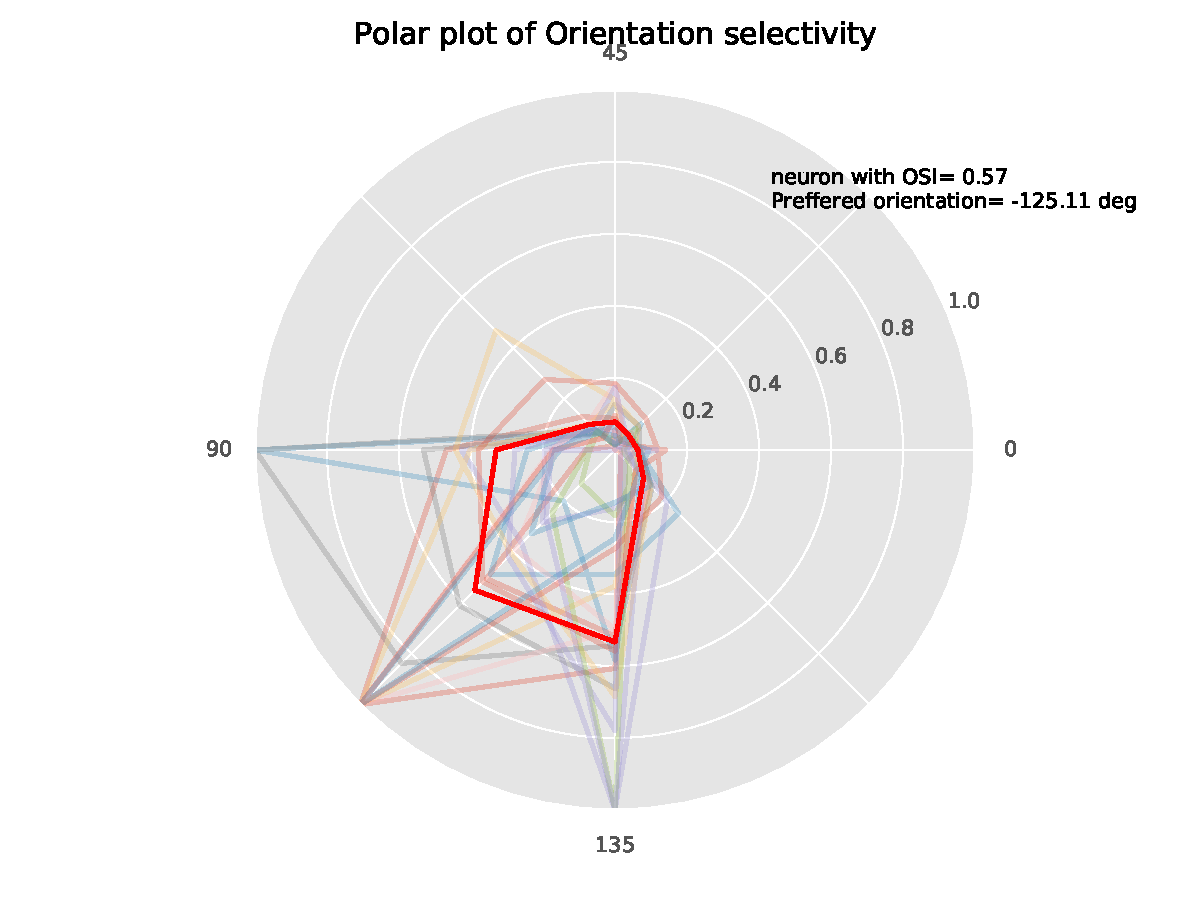
\includegraphics[width=\linewidth]{\plt/gratings_oripolar_2016_04_24_14_08_33.pdf}
    \caption{Responses plotted in orientation space}
    \label{fig:ori_simple}
  \end{subfigure}%
  \begin{subfigure}[b]{0.5\textwidth}
    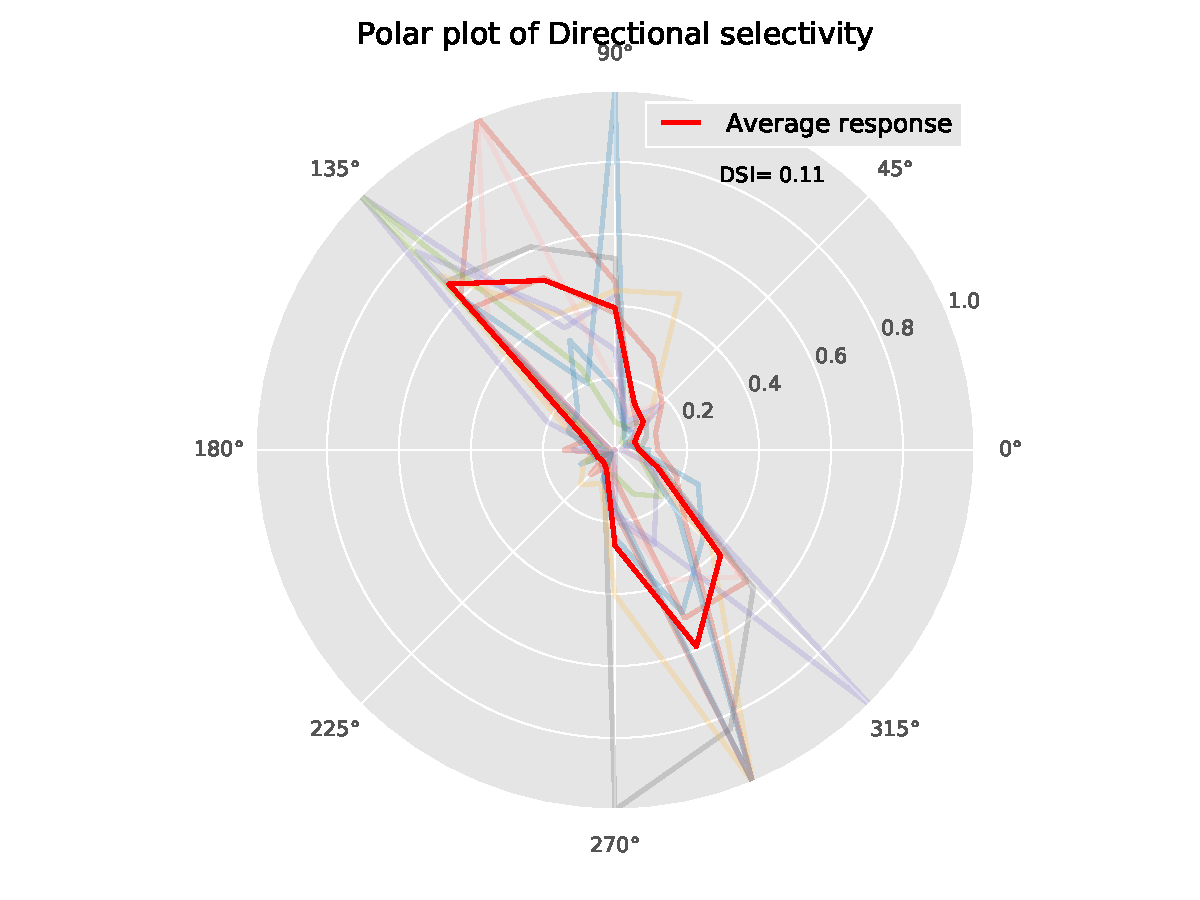
\includegraphics[width=\linewidth]{\plt/gratings_dirpolar_2016_04_24_14_08_33.pdf}
    \caption{Responses plotted in direction space}
    \label{fig:dir_simple}
  \end{subfigure}%
  \caption{Responses $R(\theta_k)$ of a simple neuron for each $\theta_k$ plotted in both orientation and direction space. Equal lobes in direction space shows direction is irrelevant to response.}\label{fig:oridir_simple}
\end{figure}

A complex neuron is expected to have high OSI and high DSI. Responses of a complex cell are plotted in orientation and direction space in Figure~\ref{fig:oridir_complex}.
\begin{figure}[h]
  \begin{subfigure}[b]{0.5\textwidth}
    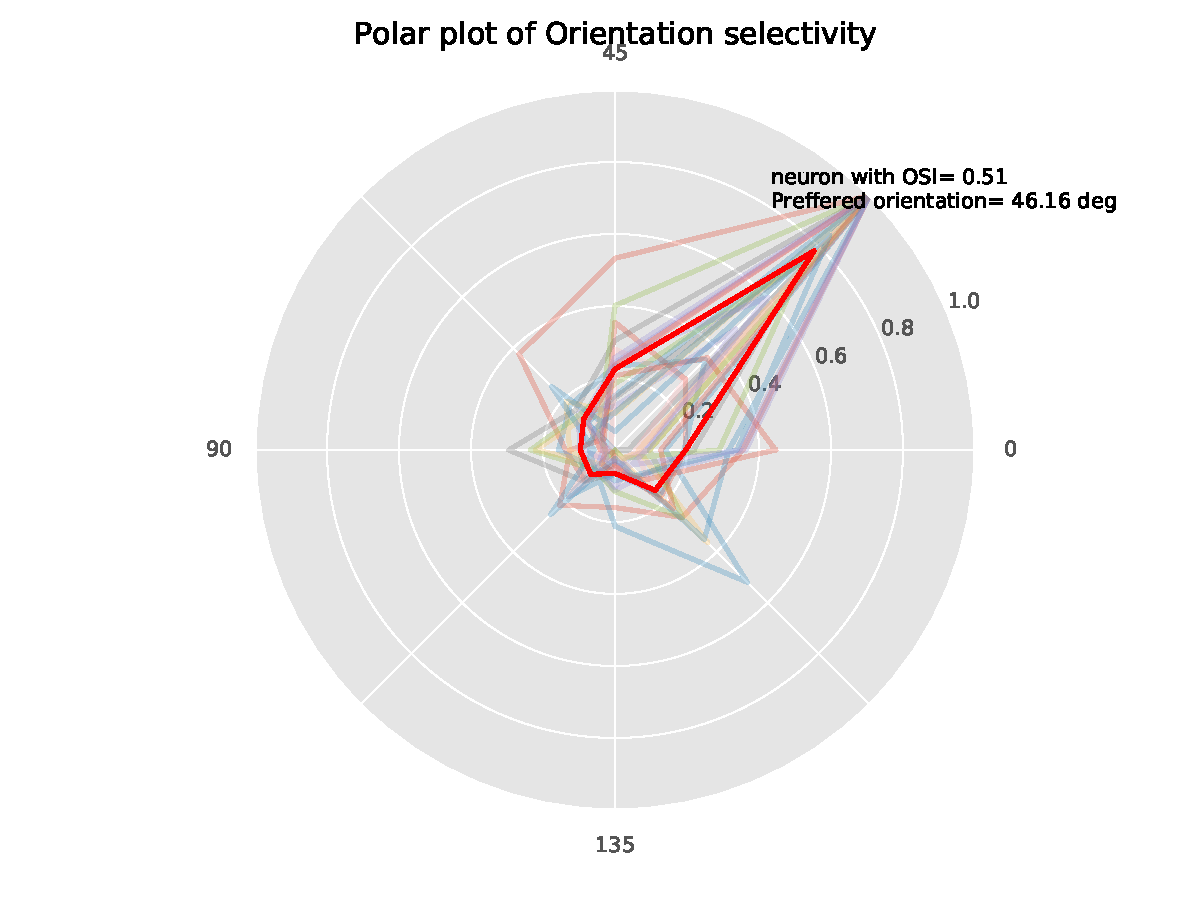
\includegraphics[width=\linewidth]{\plt/gratings_oripolar_2016_05_01_15_25_00.pdf}
    \caption{Responses plotted in orientation space}
    \label{fig:ori_complex}
  \end{subfigure}%
  \begin{subfigure}[b]{0.5\textwidth}
    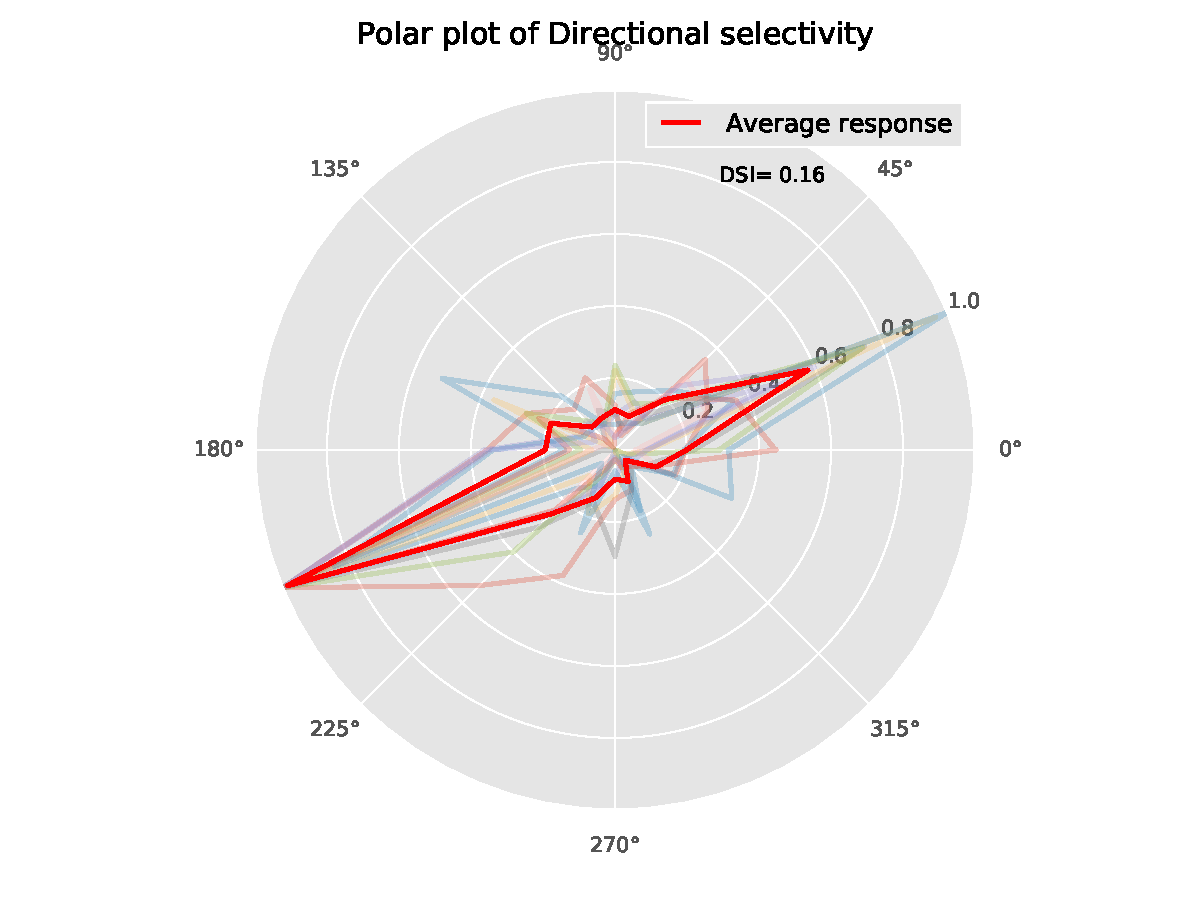
\includegraphics[width=\linewidth]{\plt/gratings_dirpolar_2016_05_01_15_25_00.pdf}
    \caption{Responses plotted in direction space}
    \label{fig:dir_complex}
  \end{subfigure}%
  \caption{Responses $R(\theta_k)$ of a complex neuron for each $\theta_k$ plotted in both orientation and direction space. Unequal lobes in direction space shows one direction is preferred than its opposite.}\label{fig:oridir_complex}
\end{figure}

An orientation insensitive neuron is expected to have low values for both OSI and DSI. Polar plots of response from an unselective cell in orientation and direction space is shown in Figure~\ref{fig:oridir_unsel}.
\begin{figure}[h]
  \begin{subfigure}[b]{0.5\textwidth}
    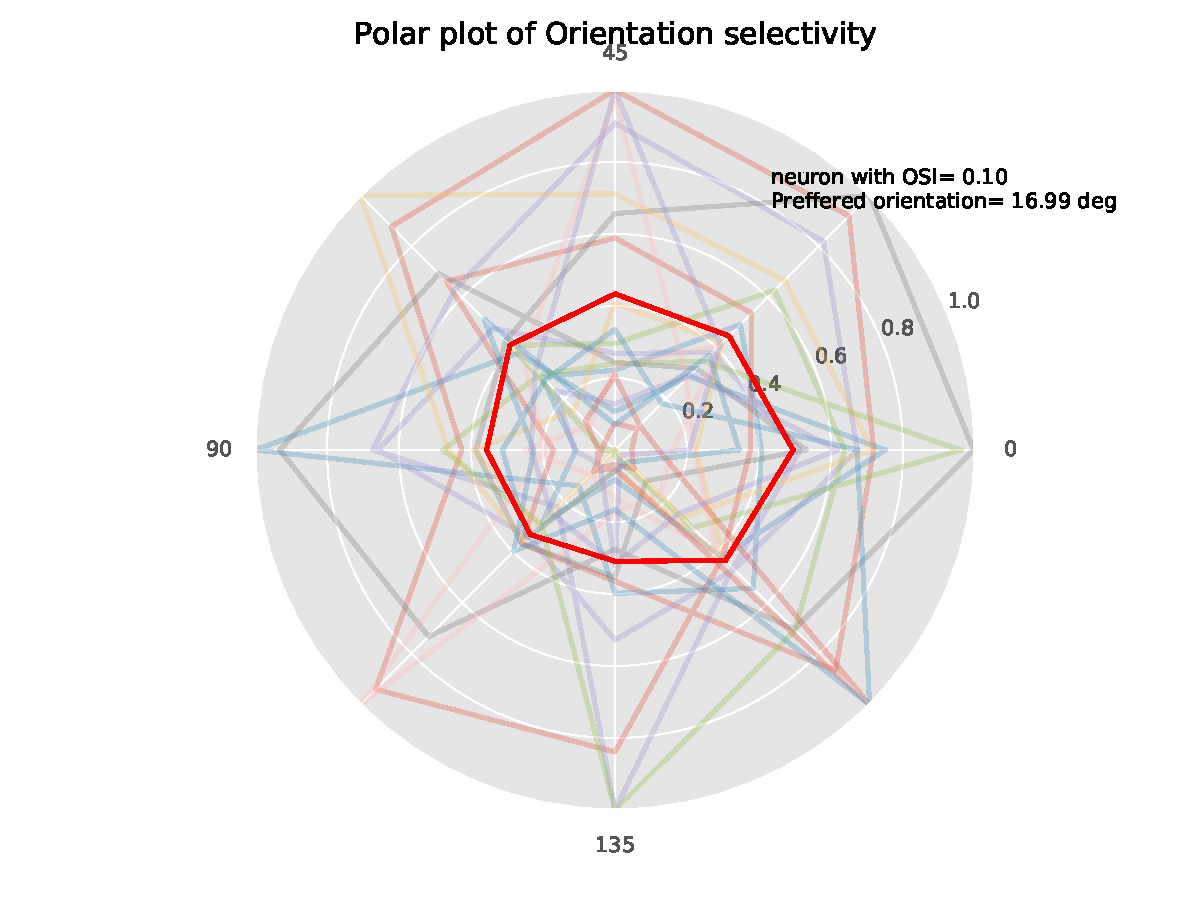
\includegraphics[width=\linewidth]{\plt/gratings_oripolar_2016_05_01_15_26_41.pdf}
    \caption{Responses plotted in orientation space}
    \label{fig:ori_unsel}
  \end{subfigure}%
  \begin{subfigure}[b]{0.5\textwidth}
    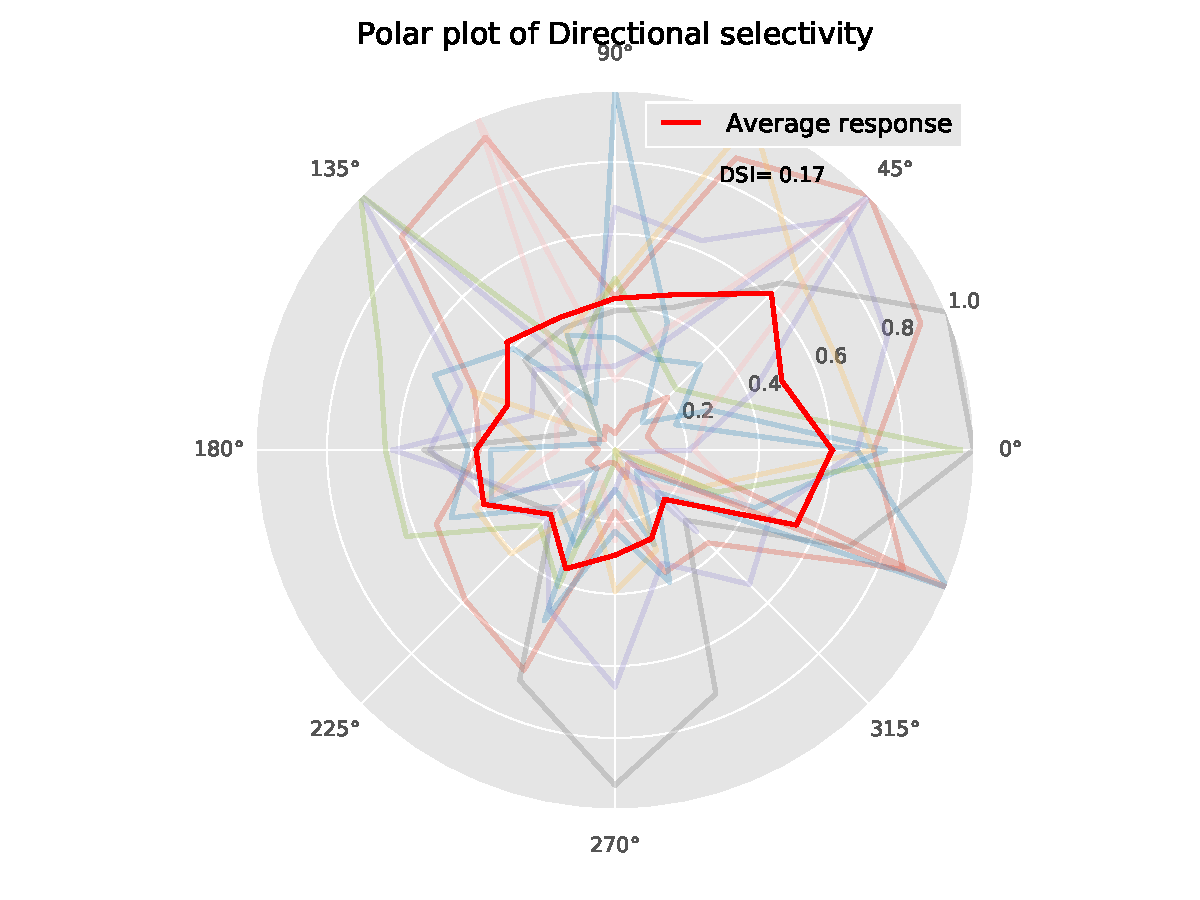
\includegraphics[width=\linewidth]{\plt/gratings_dirpolar_2016_05_01_15_26_41.pdf}
    \caption{Responses plotted in direction space}
    \label{fig:dir_unsel}
  \end{subfigure}%
  \caption{Responses $R(\theta_k)$ of a an orientation insensitive neuron for each $\theta_k$ plotted in both orientation and direction space. Similar responses to all orientations shows absence of selectivity.}\label{fig:oridir_unsel}
\end{figure}
% section quantifying_orientation_and_directional_selectivity (end)

\section{Modeling neuronal response} % (fold)
\label{sec:modeling_neuronal_response_to_sinusoidal_gratings_stimuli}
Modeling the response of neuron to various orientations and visualizing is a great way to study characteristics of neurons like orientation selectivity. We can also characterize the degree of selectivity and preferred orientation from model parameters.
Orientation tuning curve is modeled using a Gaussian function with constant offset. The empirical form of the orientation tuning curve is,
$$R_o(\theta) = C + R_p \exp\left\{\frac{-||\theta-\theta_{pref}||^2}{2\sigma^2}\right\}$$
Where $R_o(\theta)$ is the time-averaged response of a neuron to angle of orientation $\theta$. Parameter $\theta_{pref}$ is the preferred orientation of the neuron. Tuning width $\sigma$  tell us how much the cell is selective. $C$ is a constant offset.

Similarly, we can model direction tuning curve using a mixture of two Gaussian functions with a constant offset. 
$$R_d(\theta) = C + R_p \exp\left\{\frac{-||\theta-\theta_{pref}||^2}{2\sigma_1^2}\right\} + R_n \exp\left\{\frac{-||\theta-\theta_{null}||^2}{2\sigma_2^2}\right\}$$
Where $R_o(\theta)$ is the time-averaged response of neuron to angle of direction $\theta$. Relative magnitude of tuning widths, $\sigma_1$ and $\sigma_2$ denote the amount of directional selectivity. $C$ is a constant offset.
% section modeling_neuronal_response_to_sinusoidal_gratings_stimuli (end)

Parameters are estimated by minimizing squared sum of error. Sum of squared error is defined as:
$$SSE = \sum_{i=1}^N ||R(\theta_i) - R_o(\theta_i)||^2$$
A gradient descent algorithm finds the optimum parameters by minimizing SSE.
In Figure~\ref{fig:curvefit_complex} , tuning curves of a complex cell is modeled. The distinct peak in the orientation tuning curve shows selectivity to orientation $\theta_{pref}$. In the direction tuning curve, peaks of different magnitude shows one direction is more preferred than other.
\begin{figure}[h]
  \begin{subfigure}[b]{0.5\textwidth}
    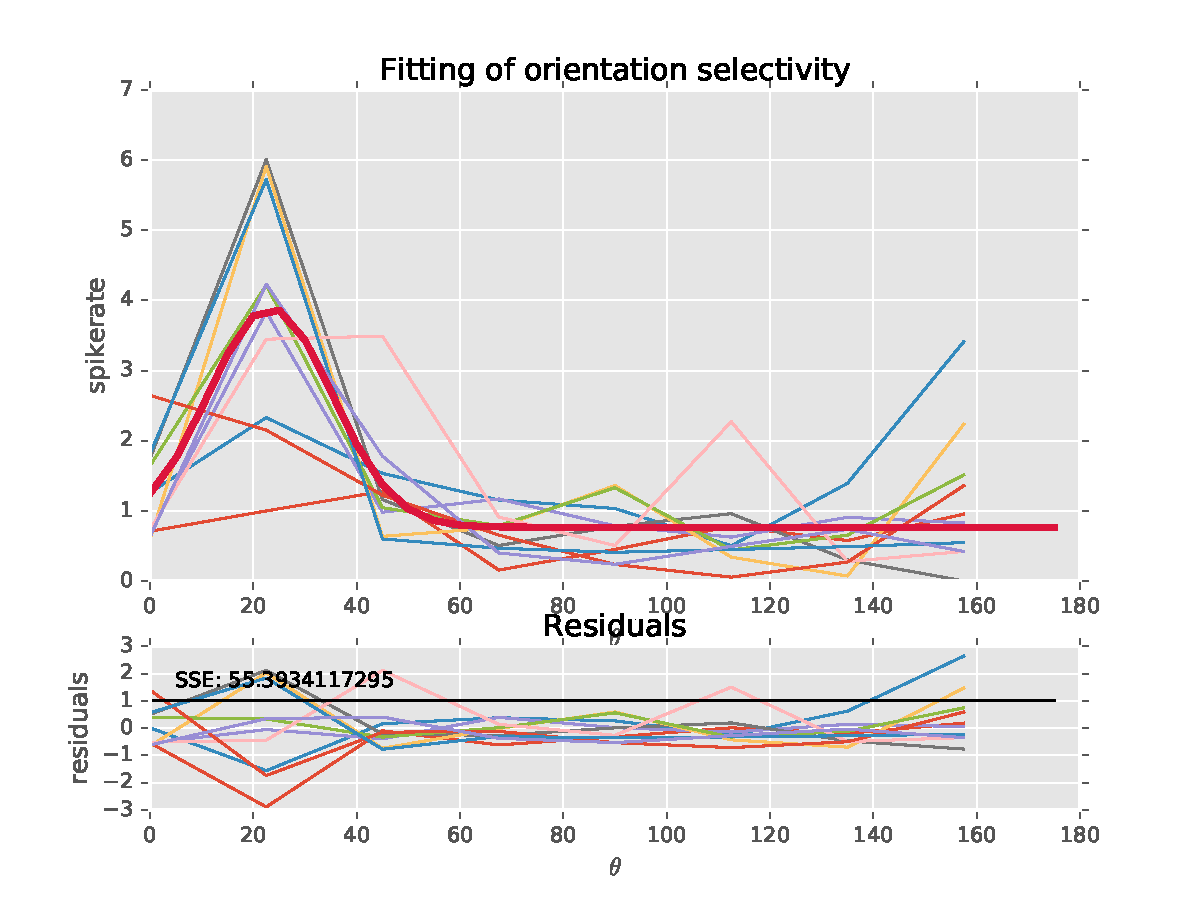
\includegraphics[width=\linewidth]{\plt/gratings_crvefit_osi_n_3_2016_05_02_12_53_03.pdf}
    \caption{Orientation tuning curve}
    \label{fig:oritune_complex}
  \end{subfigure}%
  \begin{subfigure}[b]{0.5\textwidth}
    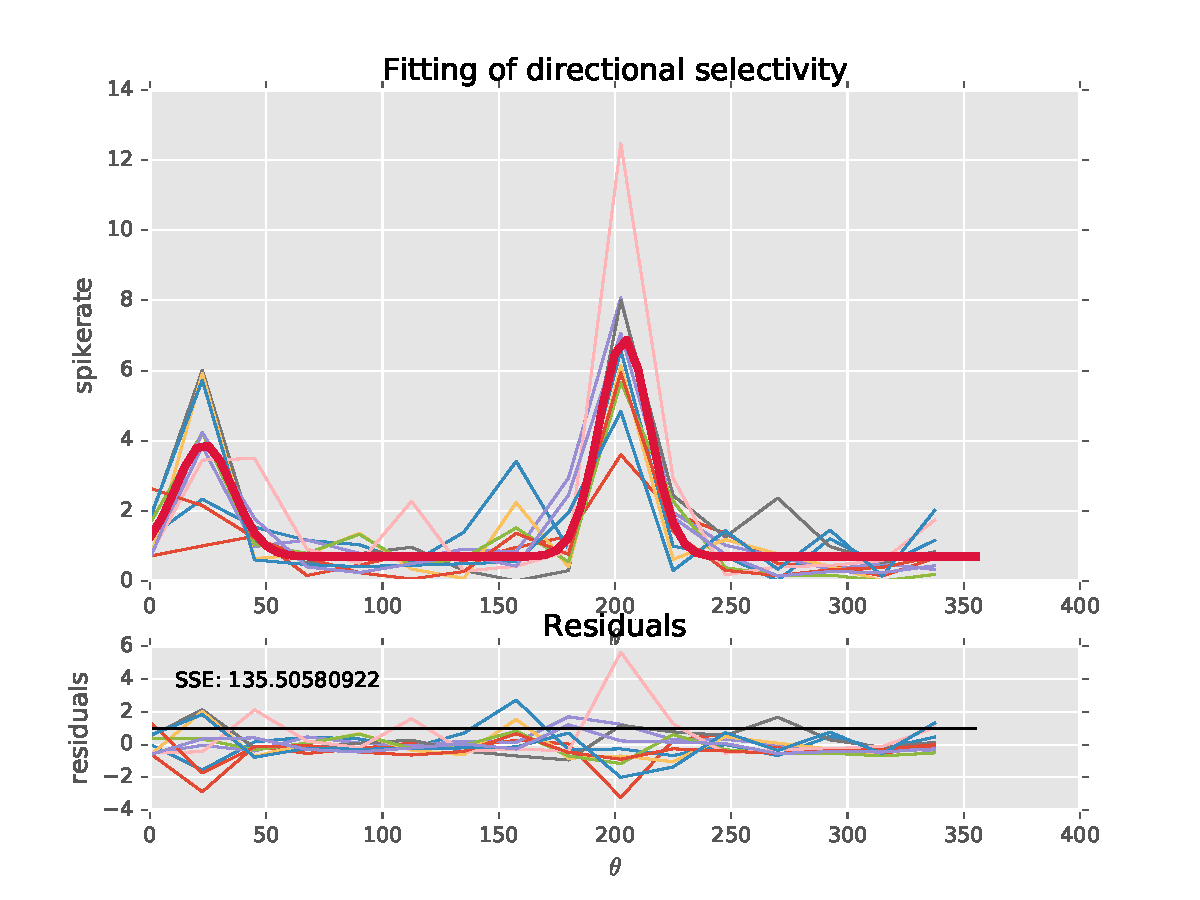
\includegraphics[width=\linewidth]{\plt/gratings_crvefit_n_3_2016_05_01_15_40_28.pdf}
    \caption{Direction tuning curve}
    \label{fig:dirtune_complex}
  \end{subfigure}%
  \caption{Fit of orientation and direction tuning curves of a neuron. The distinct peak in the orientation tuning curve shows selectivity to orientation $\theta_{pref}$. Different $\sigma_1$ and $\sigma_2$ in direction tuning curve shows direction sensitive cell. - Thus a complex cell}\label{fig:curvefit_complex}
\end{figure}
In Figure~\ref{fig:curvefit_simple} , tuning curves of a complex cell is modeled. The distinct peak in the orientation tuning curve shows selectivity to orientation $\theta_{pref}$. In the direction tuning curve, peaks of same magnitude shows of stimuli direction is irrelevant.
\begin{figure}[h]
  \begin{subfigure}[b]{0.5\textwidth}
    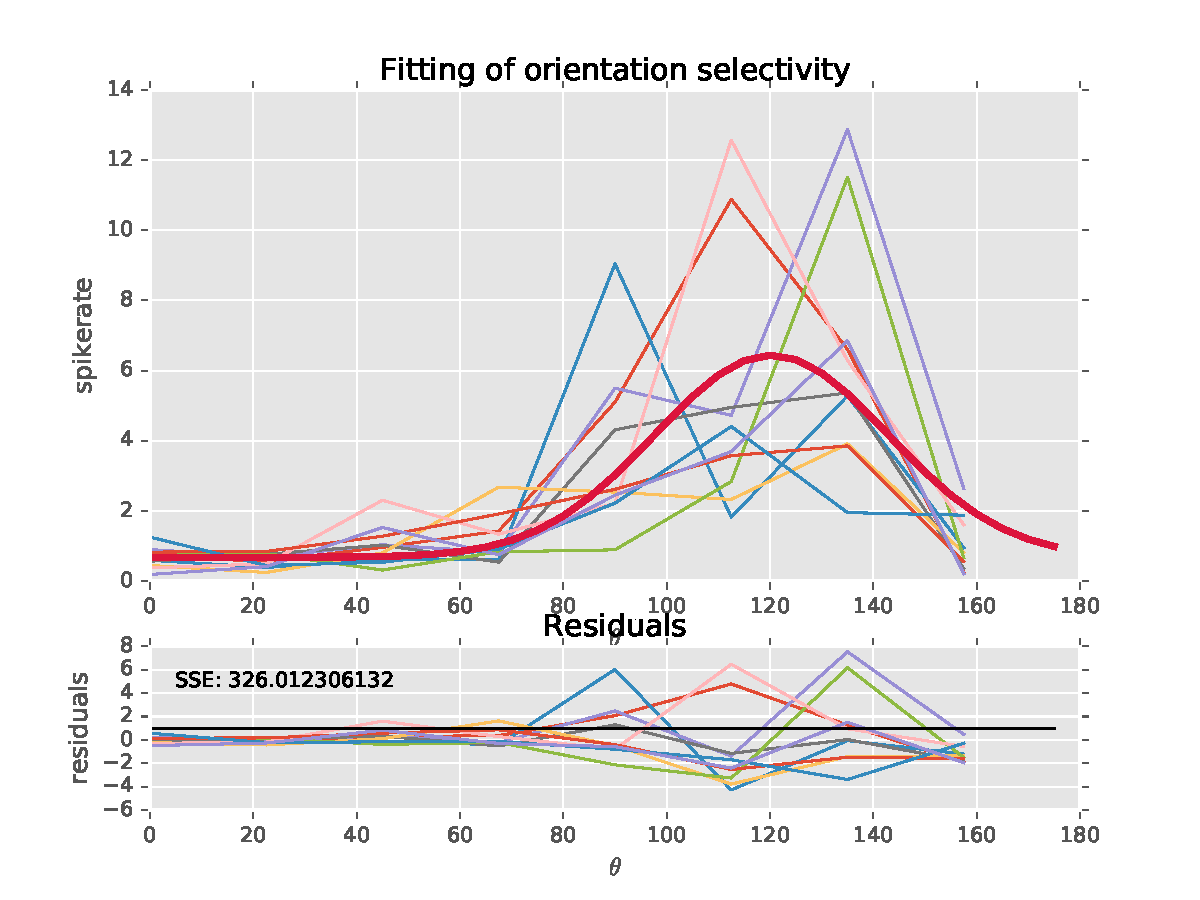
\includegraphics[width=\linewidth]{\plt/gratings_crvefit_osi_n_0_2016_05_02_12_52_43.pdf}
    \caption{Orientation tuning curve}
    \label{fig:oritune_simple}
  \end{subfigure}%
  \begin{subfigure}[b]{0.5\textwidth}
    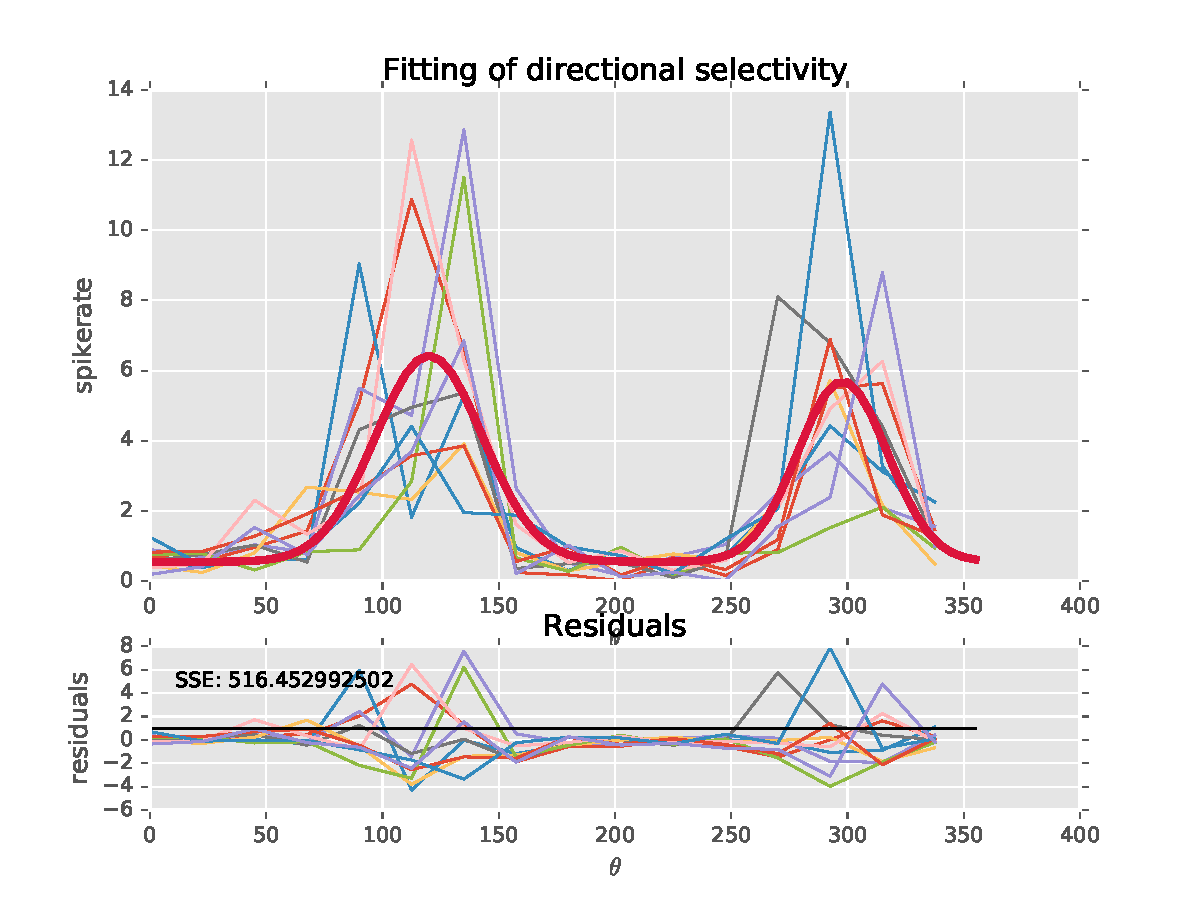
\includegraphics[width=\linewidth]{\plt/gratings_crvefit_n_0_2016_05_01_15_40_26.pdf}
    \caption{Direction tuning curve}
    \label{fig:dirtune_simple}
  \end{subfigure}%
  \caption{Fit of orientation and direction tuning curves of a neuron. The distinct peak in the orientation tuning curve shows selectivity to orientation $\theta_{pref}$. Similar $\sigma_1$ and $\sigma_2$ in direction tuning curve direction of stimuli is irrelevant. - Thus a simple cell}\label{fig:curvefit_simple}
\end{figure}
\section{Finding similarly tuned neurons} % (fold)
\label{sec:finding_similarly_tuned_neurons}
Receptive field of a neuron in V1 consists of a subset of neurons in one layer below it. Those neurons in turn have a receptive field. By following down layers by layer, we can find a visual field for each neuron in V1. Orientation selectivity of neurons in V1 detects edges and their orientation in the visual field. By studying similarly tuned neurons, we can get an insight to redundancy of coding and distribution of functionally similar cells in V1.

Similarly tuned cells are expected to have similar response to different stimuli orientations. A good correlation between responses $R(\theta_k)$ of two neurons represents similarly tuned cells. Even after having same preferred orientations, the neurons could have different degree of selectivity. We would like to find similarly tuned neurons which have an `acceptable' OSI.

Pearson correlation between each pair of neurons in a mice are computed and plotted in Figure~\ref{fig:corr}. The neurons in both axes are sorted in order of decreasing OSI values. The neuron pairs that occupy bottom left of the Figure~\ref{fig:corr} are the ones we are interested in. Finally to find neurons similar to a particular neuron, choose the row corresponding to the neuron and all the neurons in that row having good correlation value and an acceptable OSI. Figure~\ref{fig:tunecurves} shows tuning curves of some neurons retrieved from correlation study.
\begin{figure}[h]
  \centering
  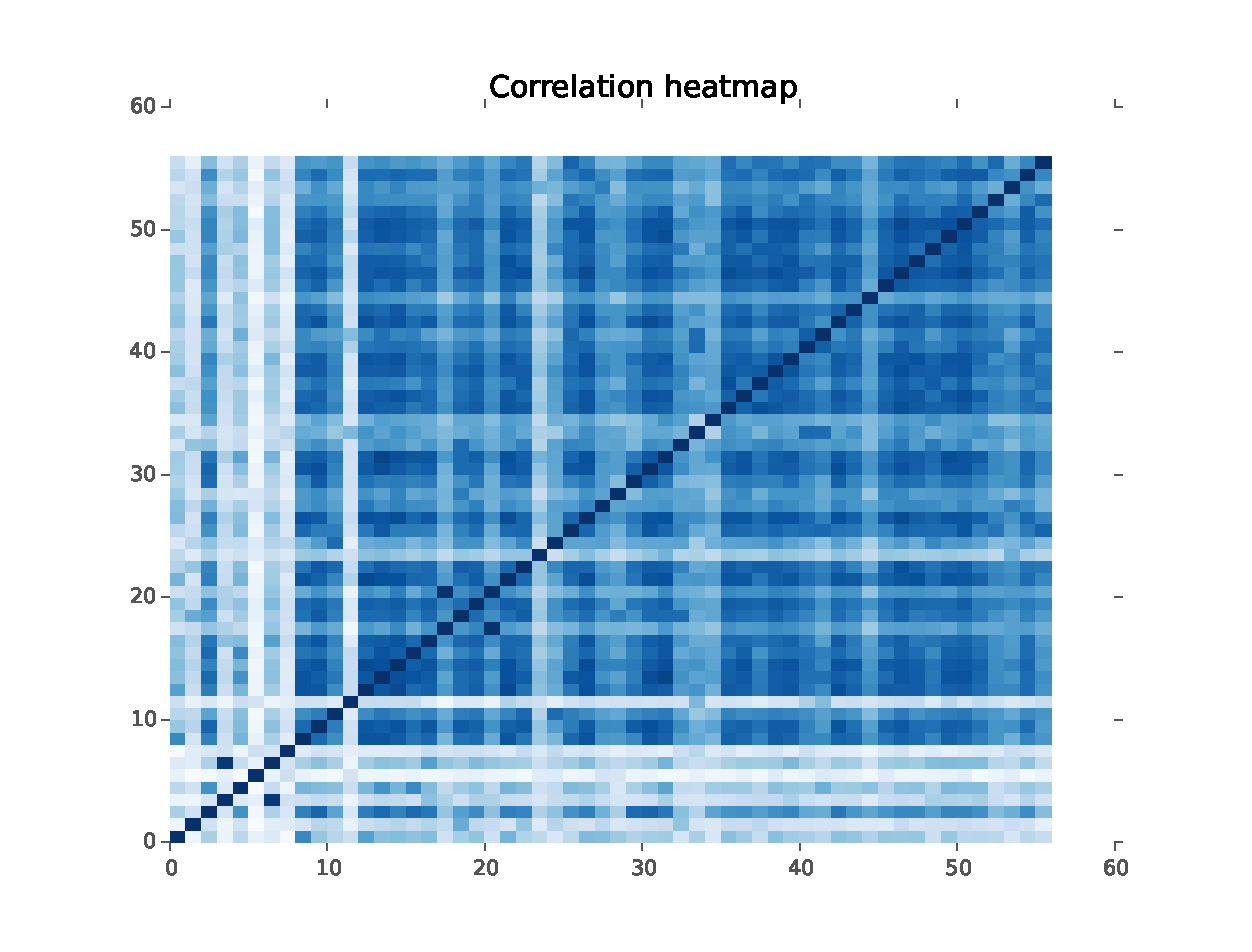
\includegraphics[width=.9\linewidth]{\plt/tuningCorr_desc_civar_m2}
  \caption{Pairwise Pearson correlation of neurons. Both axes are sorted in decreasing order of OSI.}
  \label{fig:corr}
\end{figure}
\begin{figure}[h]
  \centering
  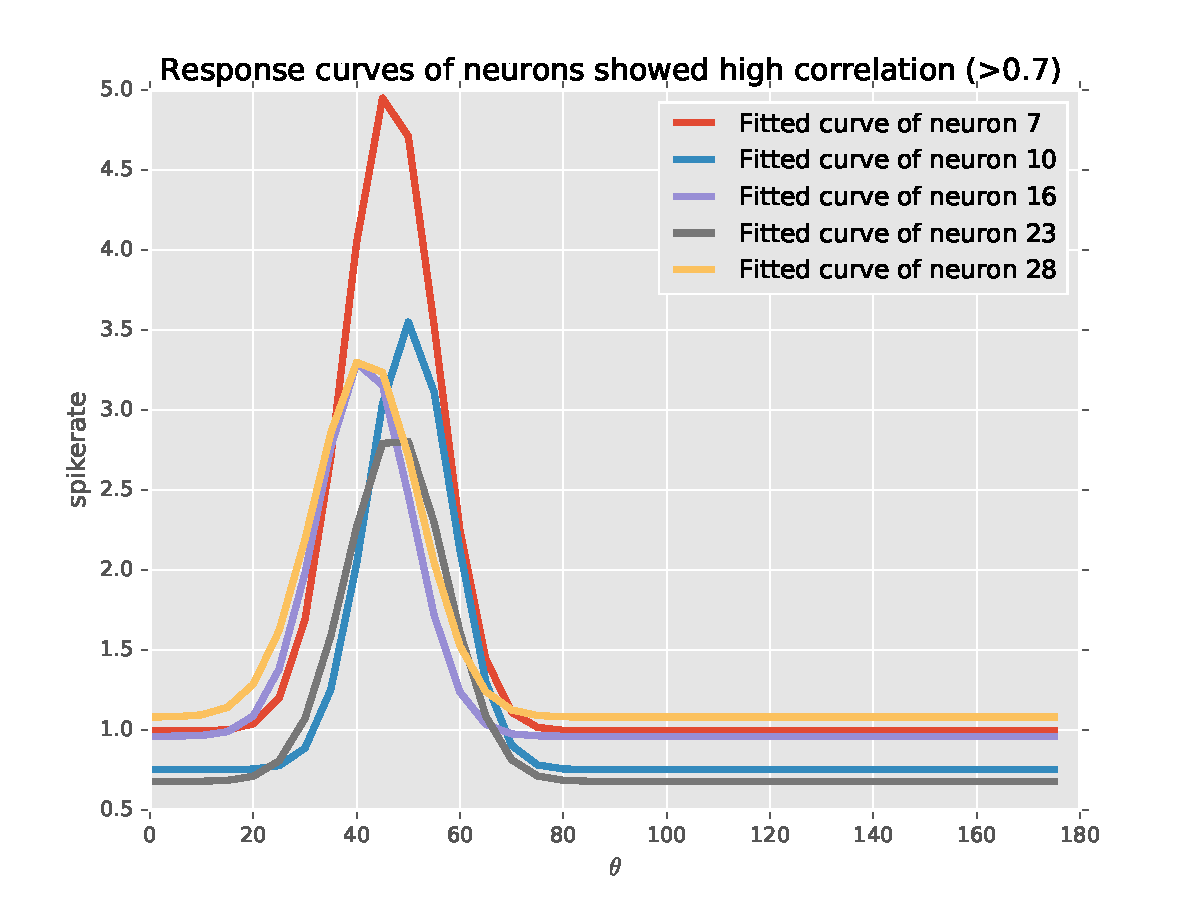
\includegraphics[width=.9\linewidth]{\plt/gratings_sel_model_2016_05_02_15_57_20.pdf}
  \caption{Orientation tuning curves of some neurons retrieved from correlation study. All of them have a same preferred orientation.}
  \label{fig:tunecurves}
\end{figure}

\section{Study of principal components} % (fold)
\label{sec:study_of_correlation}
Information contained in the visual stimuli reaches V1 after it pass through lower layers. Basic features like intensity, simple gradient of the visual scene are captured by neurons in the lower layers. Edges and motion of edges in the stimuli are represented by orientation and direction sensitive neurons in V1. With Principal Component Analysis (PCA) we aim to study the tightness of information representation. A subset of neurons ($\sim 60$) in V1 are sampled at 20Hz for 6 seconds during the experiment. We analyze principal components of the responses to find redundancy in these responses. The number of uncorrelated principal components which capture `most' of the variance in data can determine amount of redundancy.

Principal Component Analysis is an orthogonal transformation of possibly correlated observations to linearly uncorrelated components called principal components.  The principal components are orthogonal because they are the eigenvectors of the covariance matrix, which is symmetric. The first principal component captures largest variance and decreases further on. By observing number of components that needs to capture a desired variance, we can tell correlations in the data. Transforming original data to new orthogonal basis gives a representation which has dimension less than or equal to the number of original dimension. Reconstructing original data from transformed data also indicates amount of correlation in original data.

Here we take number of neurons as feature dimension. Possibility of a valid reduction will imply that same information can be represented with less number of neurons. The responses for each neuron is averaged across trials.  PCA is done on the data to find ratio between number of principal components and variance explained. Figure~\ref{img:pca} shows variance explained ratio for signals from a mouse presented with a drifting sinusoidal grating visual stimuli. The original data was transformed to principal components basis with a subset of principal components. Attempting to reconstructing original data from transformed data produces an error. The reconstruction error depends on number of chosen subset of principal components. Figure shows reconstruction error for different number of principal components. As we increase number of principal components, the error decreases. And finally as the number components equals the original feature dimension, reconstruction error vanish.
\begin{figure}
    \centering
    \begin{subfigure}[b]{.48\textwidth}
        \centering
        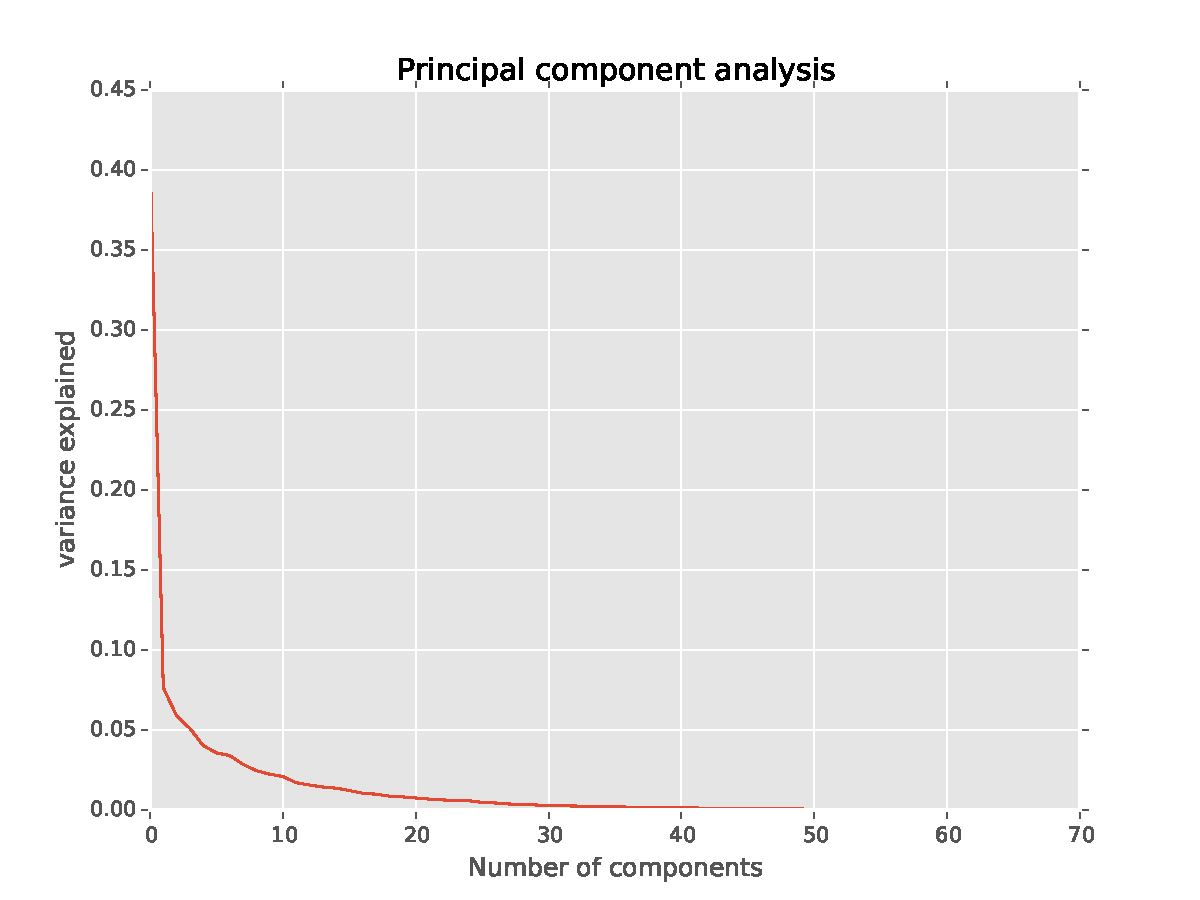
\includegraphics[width=\linewidth]{\plt/subsetbMain_pcaPlot_2016_02_05_15_41_05.pdf}
        \caption{Variance captured by components}
        \label{img:pca}
    \end{subfigure}
    ~
    \begin{subfigure}[b]{.48\textwidth}
        \centering
        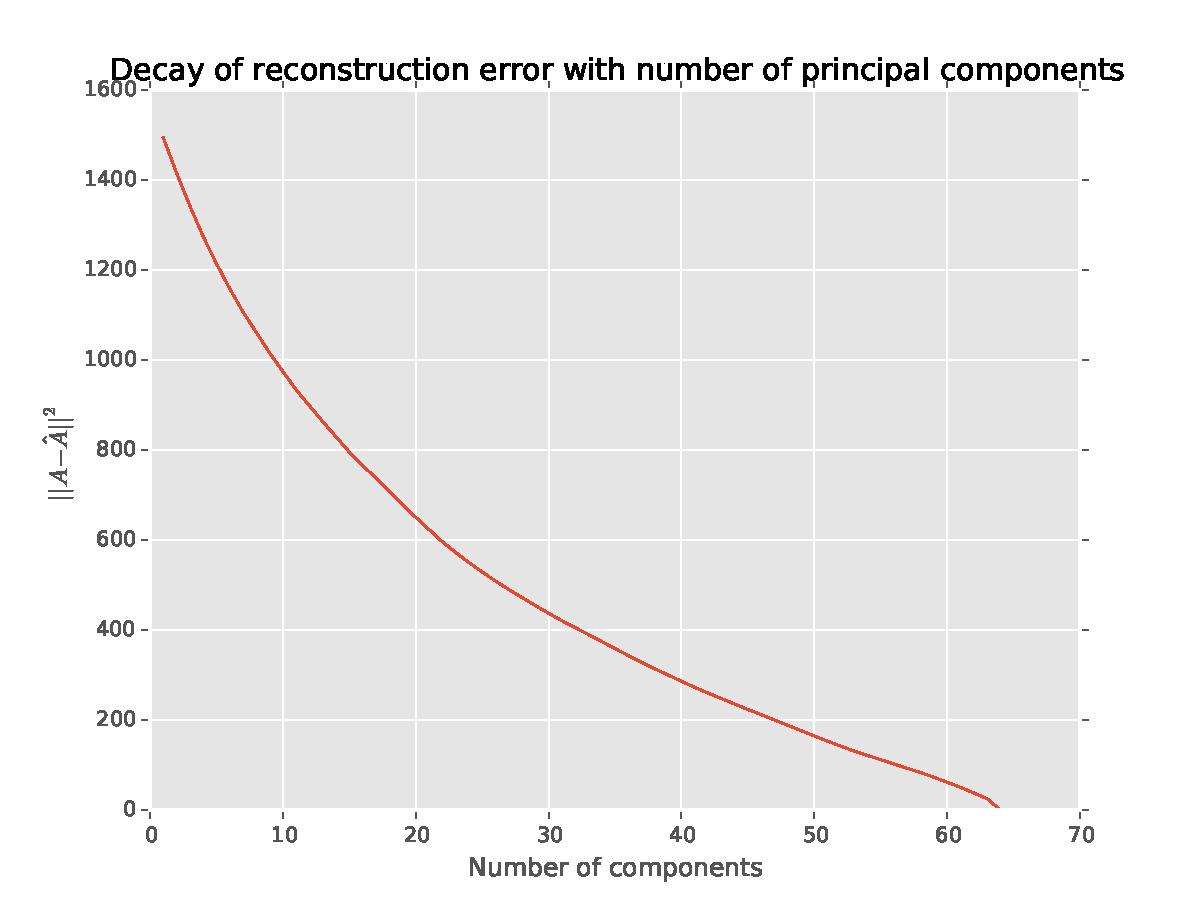
\includegraphics[width=\linewidth]{\plt/subsetbMain_errPlot_2016_02_12_12_42_39.pdf}
        \caption{Decay of reconstruction error}
        \label{img:reconstruction}
    \end{subfigure}
    \caption{Principal Component Analysis of response of neuron to drifting sinusoidal grating stimuli.}
\end{figure}
\section{Study of Reliability} % (fold)
\label{sec:study_of_reliability}
Information encoding in primary visual cortex is a complex process due to intrinsic neuronal variability. Analysis of intertrial reliability of information encoding in neurons is the first step into understanding coding mechanism of V1. The degree of trial-to-trial variability in a response is commonly measured in terms of reliability. A neuron is said to be reliable if it fires the same number of precisely timed spikes on every repetition of a stimulus [\cite{tiesinga2008regulation}].

The devised experiment measures calcium concentration in neurons rather than spike rate. Trial to trial reliability can be computed using correlation between calcium responses of each trial. When a visual stimuli is presented $T$ times to a mouse, we can compute response reliability $R_A$ of a neuron to the stimuli $A$ as
$$R_A = \frac{2}{T^2 - T}\sum_{i=1}^T \sum_{j=i+1}^T \rho(f_{i, A}, f_{j, A})$$
where $f_{i, A}$ is the response of neuron to $i^{th}$ trial of movie A and $\rho$ is the Pearson correlation.

The study was done for 48 neurons in a mice and the response reliability is plotted in Figure~\ref{img:ra} for each neuron. It is evident that response reliability for most of neurons are small. The study shows responses of neurons in V1 are not robust because of intrinsic noise. If the whole sequences is not reliable, could there be subsequences that are reliable? We will explore it in coming chapters by searching for common subsequences.
\begin{figure}[h]
    \centering
    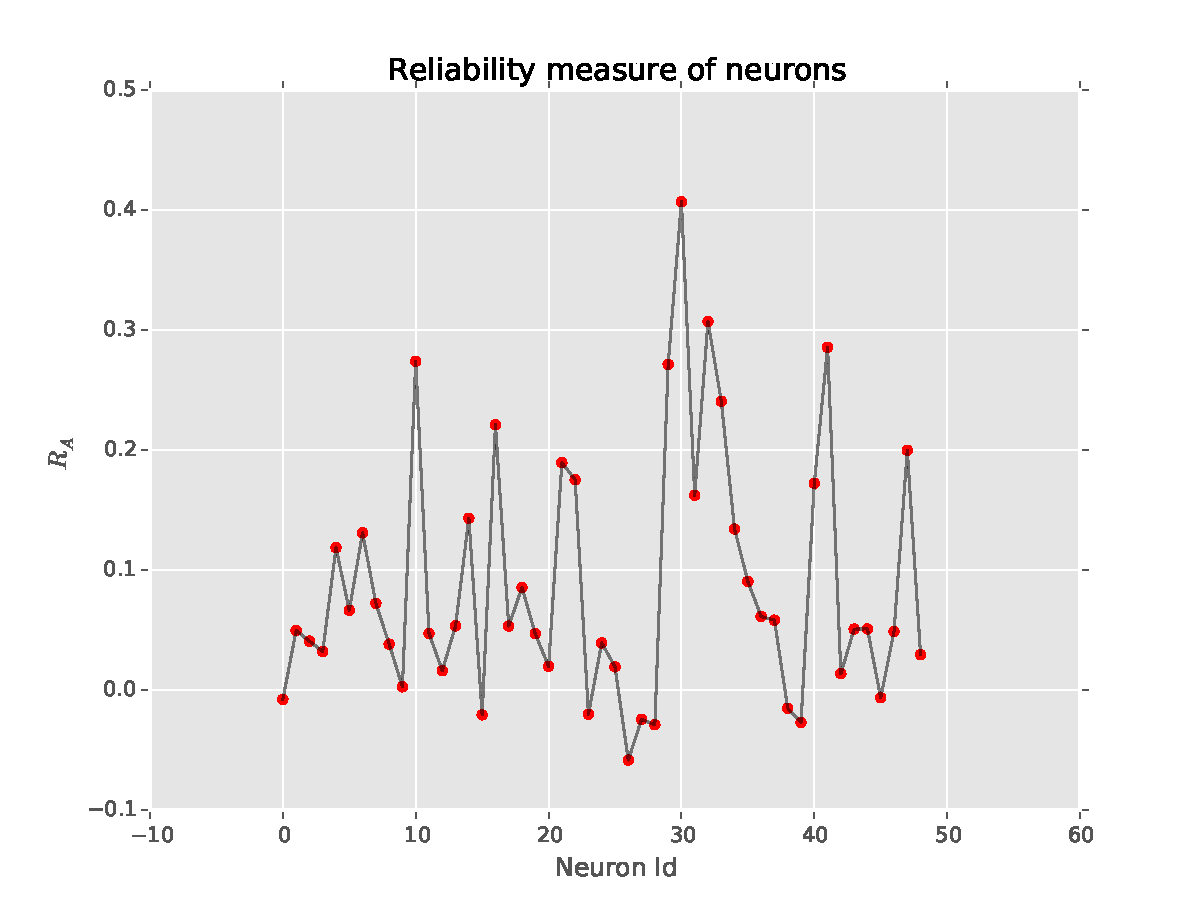
\includegraphics[width=.6\linewidth]{\plt/reliabMain_raPlot_2016_02_05_13_25_56.pdf}
    \caption{Reliability measure $R_A$ for different neurons}
    \label{img:ra}
\end{figure} 
% section study_of_reliability (end)
% section finding_similarly_tuned_neurons (end)
%%%%%%%%%%%%%%%%%%%%%%%%%%%%%%%%%%%%%%%%%%%%%%%%%%%%%%%%%%%%%%%%%%%%%%
\chapter{Searching for Motifs}       % 6 pages
\label{chap:searchmotif}
In Music, motif is a perceivable recurring fragment. Detecting such motifs in a song tells us more about the song like its melody. In Genetics, motif is a sequence pattern of nucleotides in a longer DNA sequence. From a signal processing perceptive, motifs are signal segments that recurs in a longer signal. A valid motif should have an `acceptable' length such that it has a significance. Motif analysis is important since in every domain, occurrence of motifs shows an underlying pattern and has a meaning to it.

In the experiments performed, each neuron responses are captured as a time series sampled at 50Hz for 4 seconds. In neuron responses we define a motif as subsequence of response signal having significant length and repeats itself either in
\begin{itemize}
   \item the same response signal but in a different part \textbf{or}
   \item the response of the same neuron to a different trial \textbf{or}
   \item the response of another neuron in the same mouse \textbf{or}
   \item the response of neuron in a different mouse \textbf{and}
\end{itemize}
Analysis of motifs in neuronal signals will help us understand reliable information representation. Even if two responses of same trial has a long subsequence but not time synchronized, Study of reliability in Section~\ref{sec:study_of_reliability} will fail as the Pearson correlation coefficient will output a small value. Motivic analysis can detect such subsequences even if they are time shifted.

Study of motifs across two different neurons within a mouse can explain correlation between two neurons. Correlated neurons can represent neuronal interconnections. Correlated and synchronous activity in populations of neurons has been observed in many brain regions and has been shown to play a crucial role in cortical coding, attention, and network dynamics [\cite{rosenbaum2014correlated}]. Studying correlations between neurons is again not effective if their responses are time separated as Pearson correlation will fail. Analyzing motifs across neurons will be a better way to study neuronal correlations.

Motifs found in neurons from two \textit{different} mice will represent similar biological process both the neurons share. As the motifs found cannot be due to interconnections, they are due to similar activation mechanism of neurons. In this case, we would expect a small motif compared to motifs found between neurons within a mouse.

In this chapter, we will analyze the presence of motifs in neuronal signals. The presence of motifs will motivate us to extract the motifs and infer their significance.
\section{Cross-correlation Function} % (fold)
\label{sec:correlation_function}
Cross-correlation is a measure of similarity between two signals as a function of lag of one signal relative to the other. It is commonly used for searching a query sequence in a large reference sequence. The function calculates sliding dot product at various lags. For discrete signals, cross correlation is defined as:
$$(f \star g)[n]\ \stackrel{\mathrm{def}}{=} \sum_{m=-\infty}^{\infty} f^*[m]\ g[m+n].$$
Searching for a motif using cross-correlation function  is possible if we already have a subsequence that we suspect as a motif. To visualize correlation function in query search, we will manually select a query sequence and search for its occurrences in another neuronal response. For the scope of this chapter, we take a subsequence from the response of a `template neuron' and search for its occurrences in response of a `target neuron'.

Trial averaged responses of template and target neurons are chosen and a subset frame of former is extracted using frame ending and frame width as parameters. This query sequence is compared with target sequence as a function of lag. Figure~\ref{img:cacf} shows Cross-Correlation function between a target neuron response and a manually chosen subsequence from template neuron.
\begin{figure}[h]
    \centering
    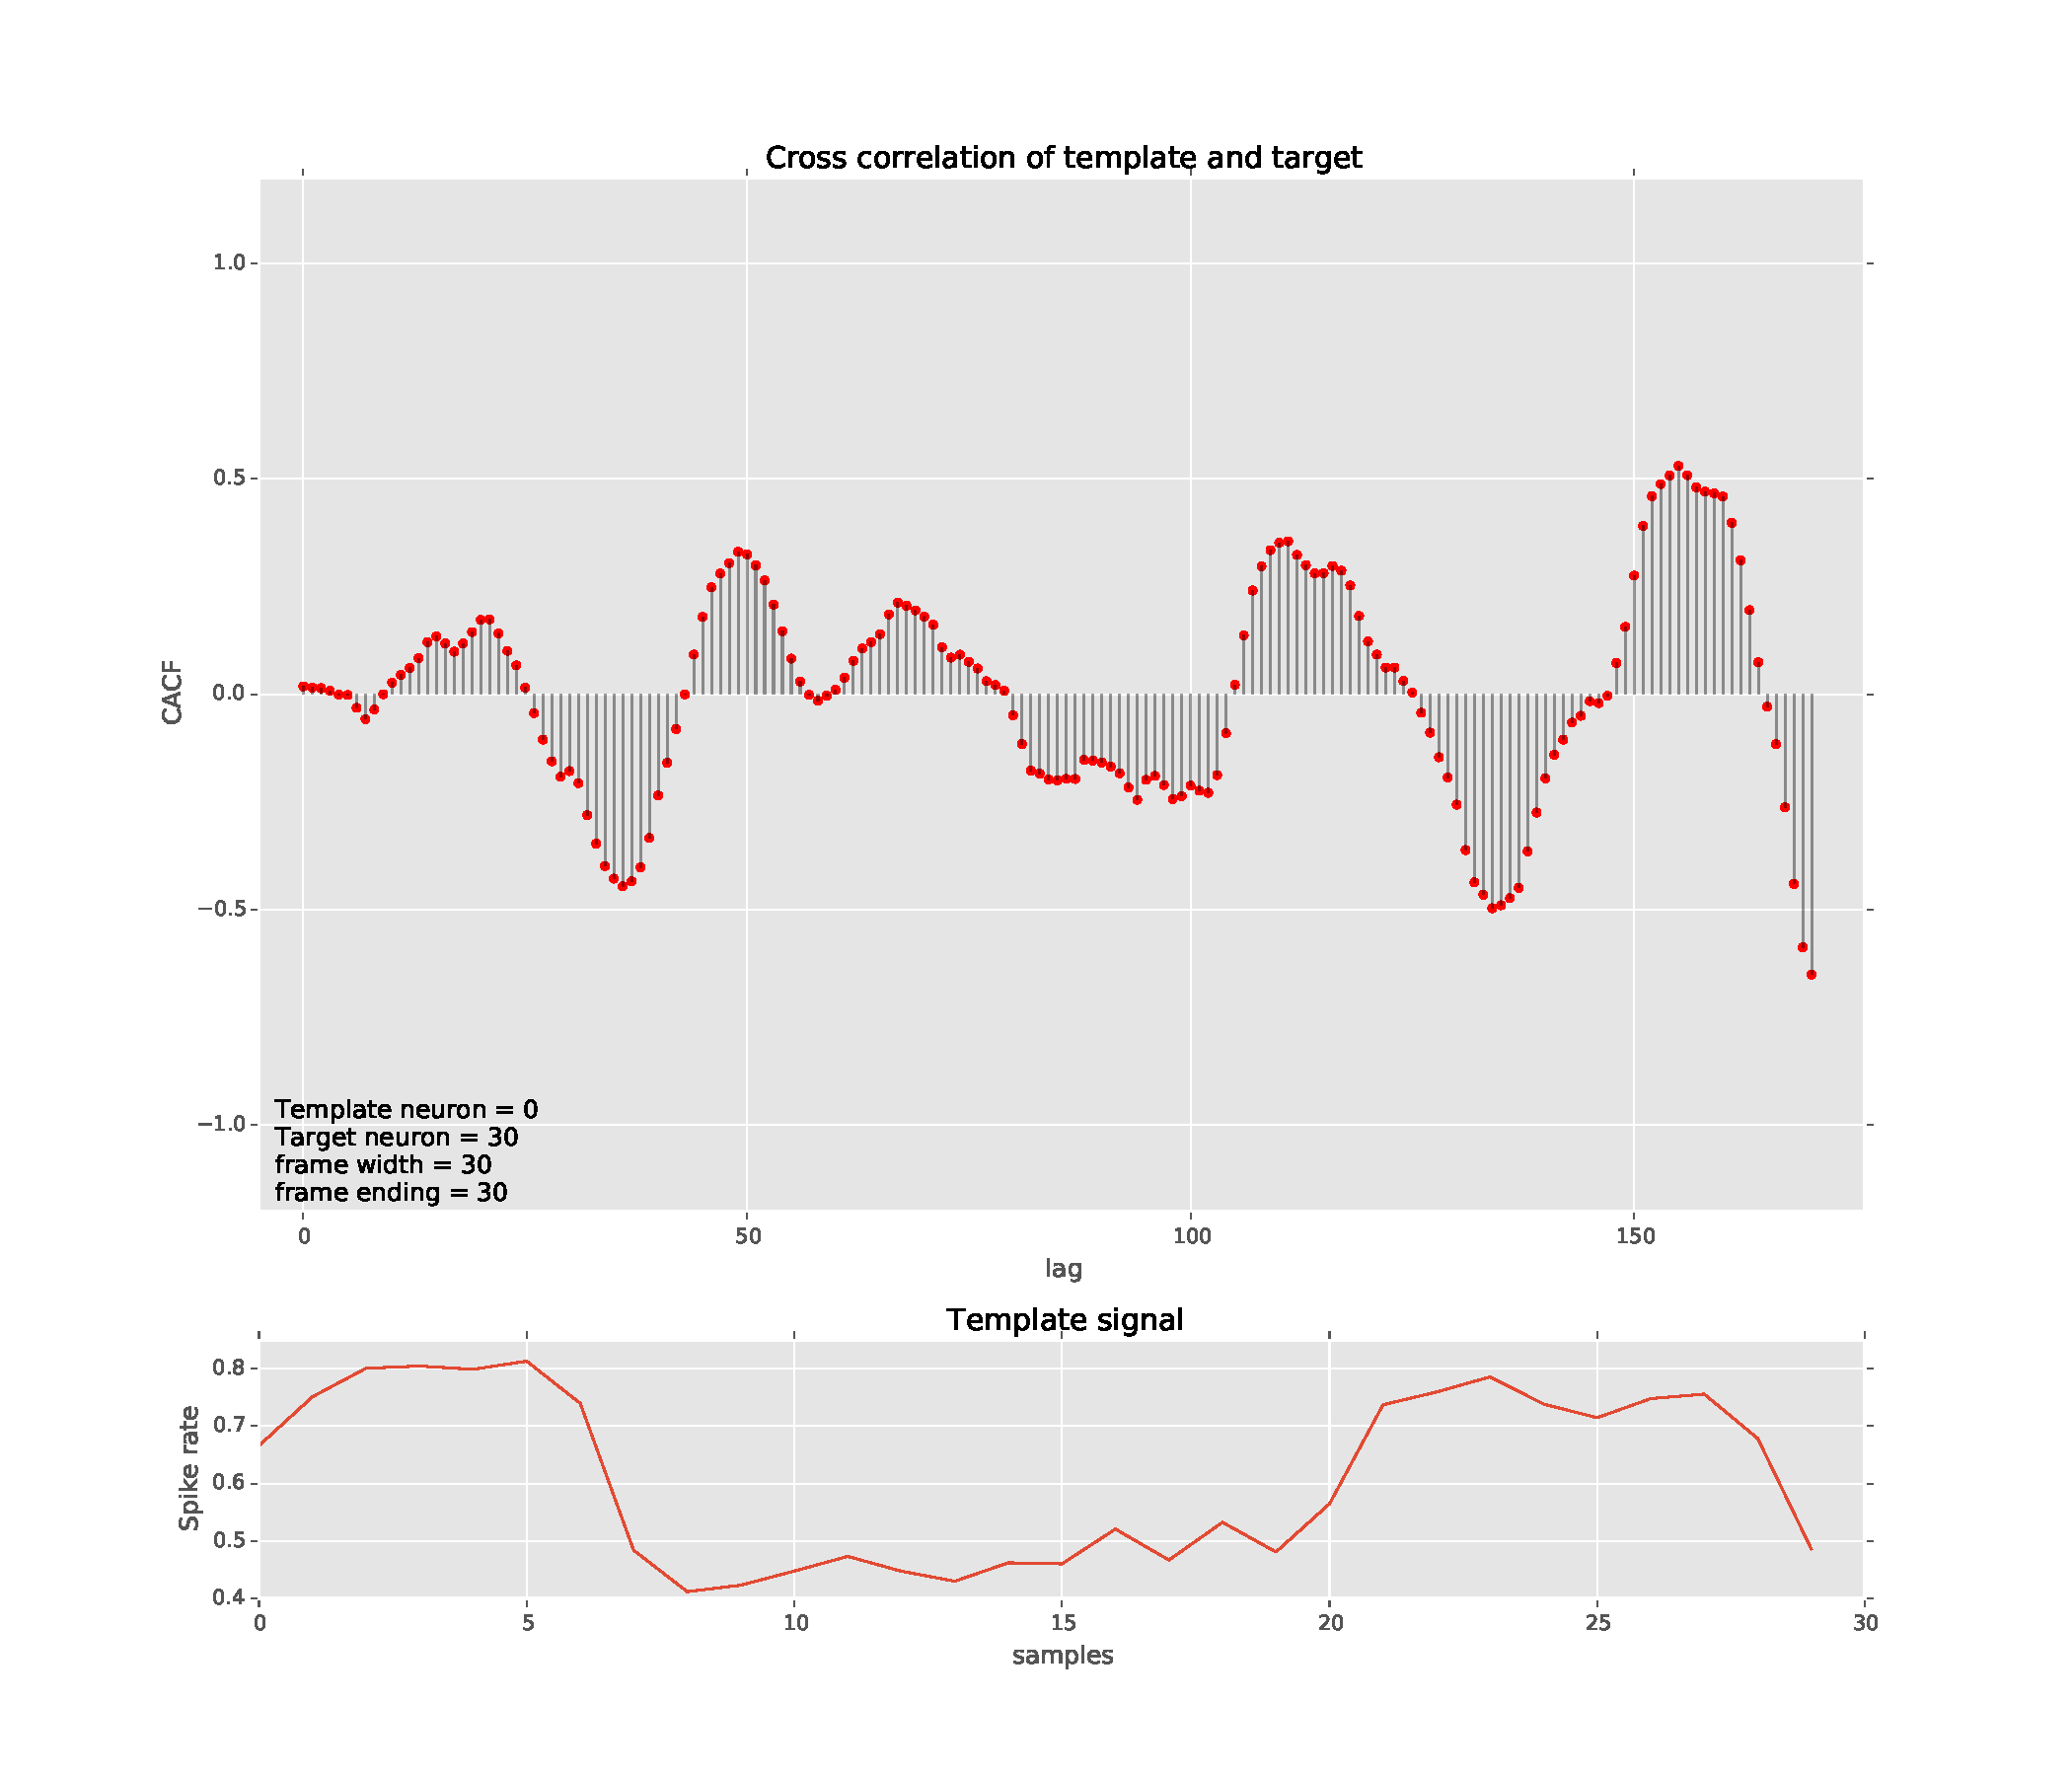
\includegraphics[width=.7\linewidth]{\plt/acfMain_acfPlot_2016_02_05_16_45_37.pdf}
    \caption{Cross-Correlation function between a target neuron response and a manually chosen subsequence from template neuron.}
    \label{img:cacf}
\end{figure}
This study is not effective as we do not know what to search for. Manually selecting a subsequence is inefficient and selected subsequence does not guarantee to be a valid motif. 
% section correlation_function (end)
\section{ACFGram} % (fold)
\label{sec:acfgram}
A spectrum describes a signal in terms of energy spread over its frequency components. A spectrogram does exactly the same but also takes time into consideration. Computing spectrogram is done by first making chunks/frames of time-domain signal which usually overlap; Magnitude of Fourier transform of each frame is computed to form magnitude spectrum of that frame. These frame spectra are stacked horizontally in increasing order of frame ending time to form a temporal dimension. The resulting frequency vs time vs magnitude representation is called spectrogram. Spectrogram enables us to study the change of spectra over time.

We formulate an analogous visualization of cross-Correlation function where the template signal changes in each frame. A frame is a subsequence of original signal with a width and frame ending parameter. Changing the frame ending successively will return overlapping frames having same width. Figure~\ref{img:framesel} shows how a frame from template signal is selected.
\begin{figure}[h]
    \centering
    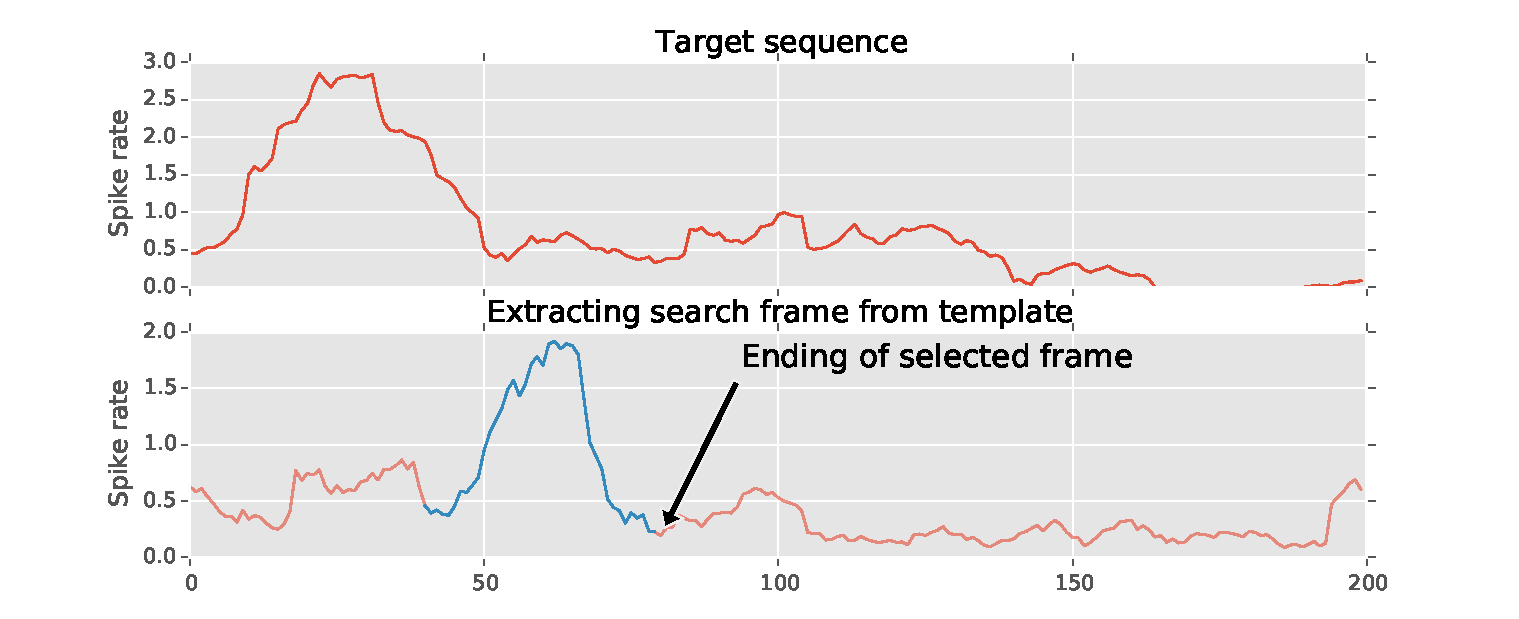
\includegraphics[width=\linewidth]{\plt/framesel.pdf}
    \caption{Extracting frame from template based on frame width and ending.}
    \label{img:framesel}
\end{figure}
Cross-Correlation of extracted frame and target signal at various lags are computed. Next frame is extracted by incrementing frame ending parameter by another parameter called frame shift. The process is then repeated for the next frames until the template sequence is exhausted. Cross-Correlation function of each frame is then stacked horizontally to form a temporal dimension. We call the resulting Time Vs Lag Vs Cross-Correlation function as ACFGram.
% $$ShYaM1193
In Section~\ref{sec:correlation_function} we varied frame width and frame ending manually to extract a signal subsequence and then queried it in target signal. ACFGram removes frame ending parameter from manual configuration. Existence of motifs will be clear if we examine ACFGram for various frame widths. The study is conducted across trials of same neuron and across different neurons.

The Figure~\ref{fig:acfgram_same}  shows ACFGram plots for template and target responses from same neuron. The study aim to find presence of repeating subsequence within a neuron's response. The length of suspected motif is varied as a parameter.
For a small frame width ($\sim 15$) the estimation of Cross-Correlation function is poor. Also such a small subsequence is not significant enough to be considered as a motif. As we Increase the frame width, repeating patterns are found which indicates the presence of repeating subsequence.
\begin{figure}[h]
  \begin{subfigure}[b]{0.5\textwidth}
    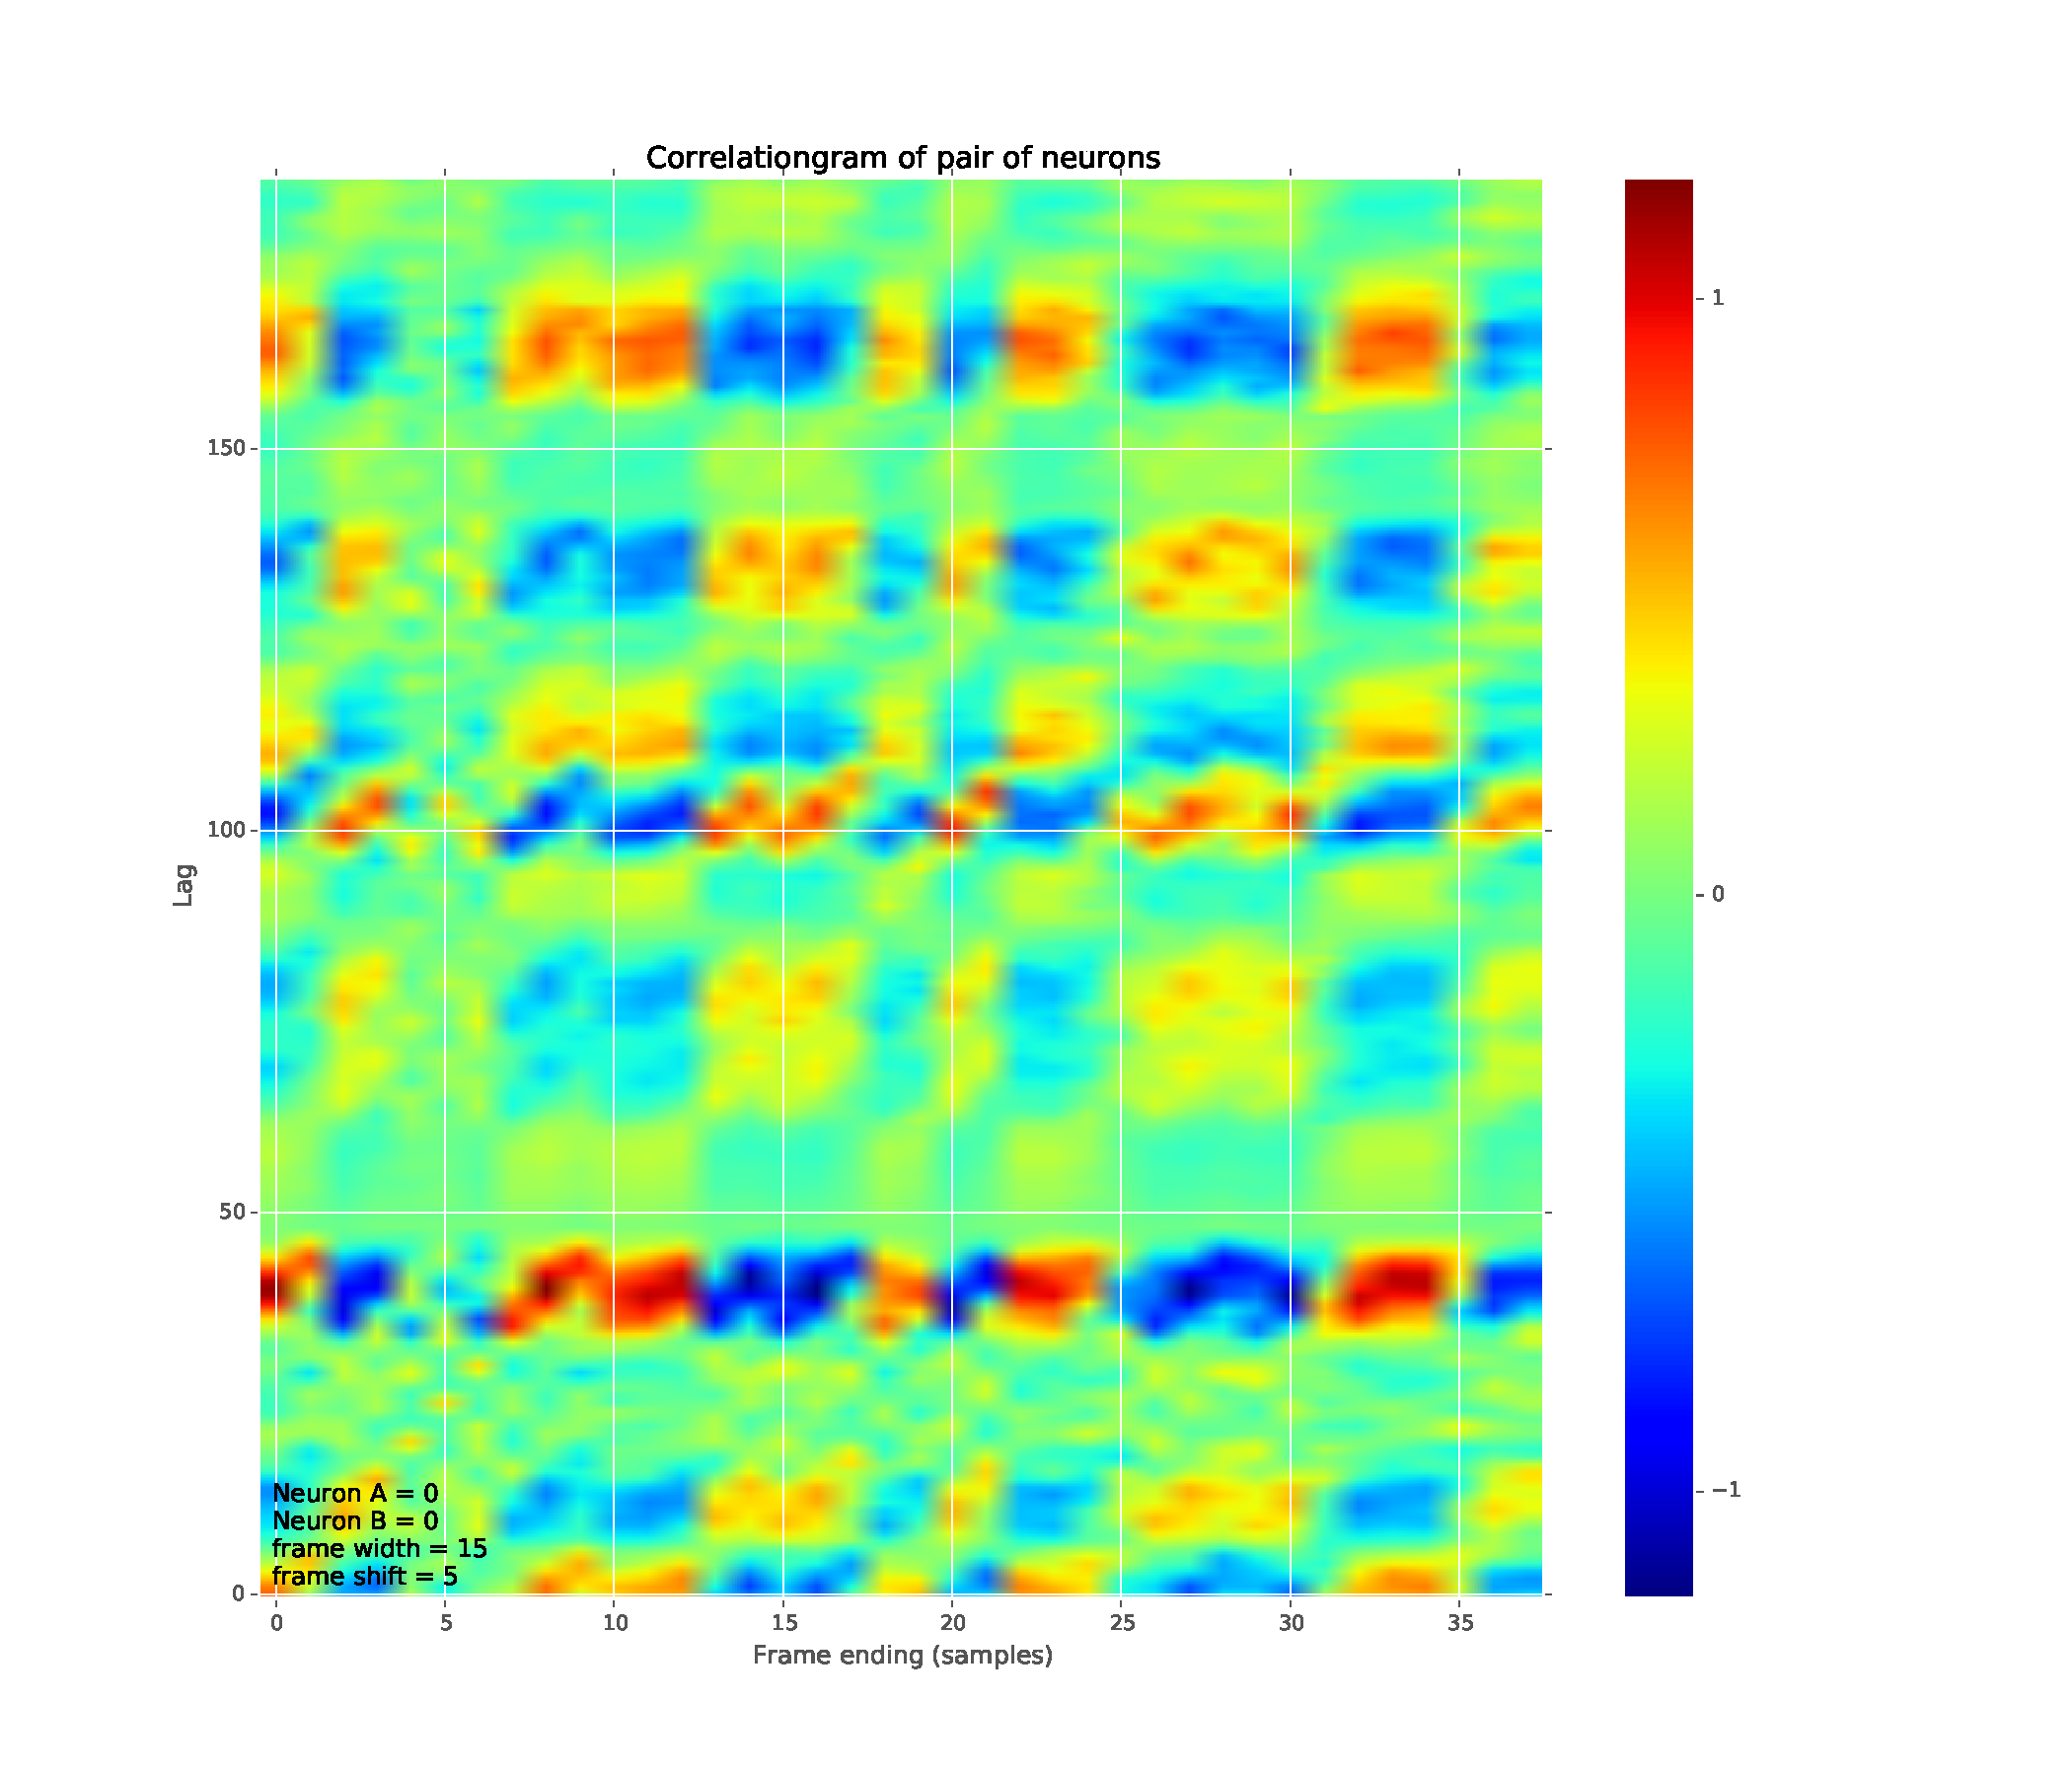
\includegraphics[width=\linewidth]{\plt/acfMain_corrGram_2016_02_05_16_49_00.pdf}
    \caption{Frame width = 15}
    \label{fig:ori_simple}
  \end{subfigure}%
  \begin{subfigure}[b]{0.5\textwidth}
    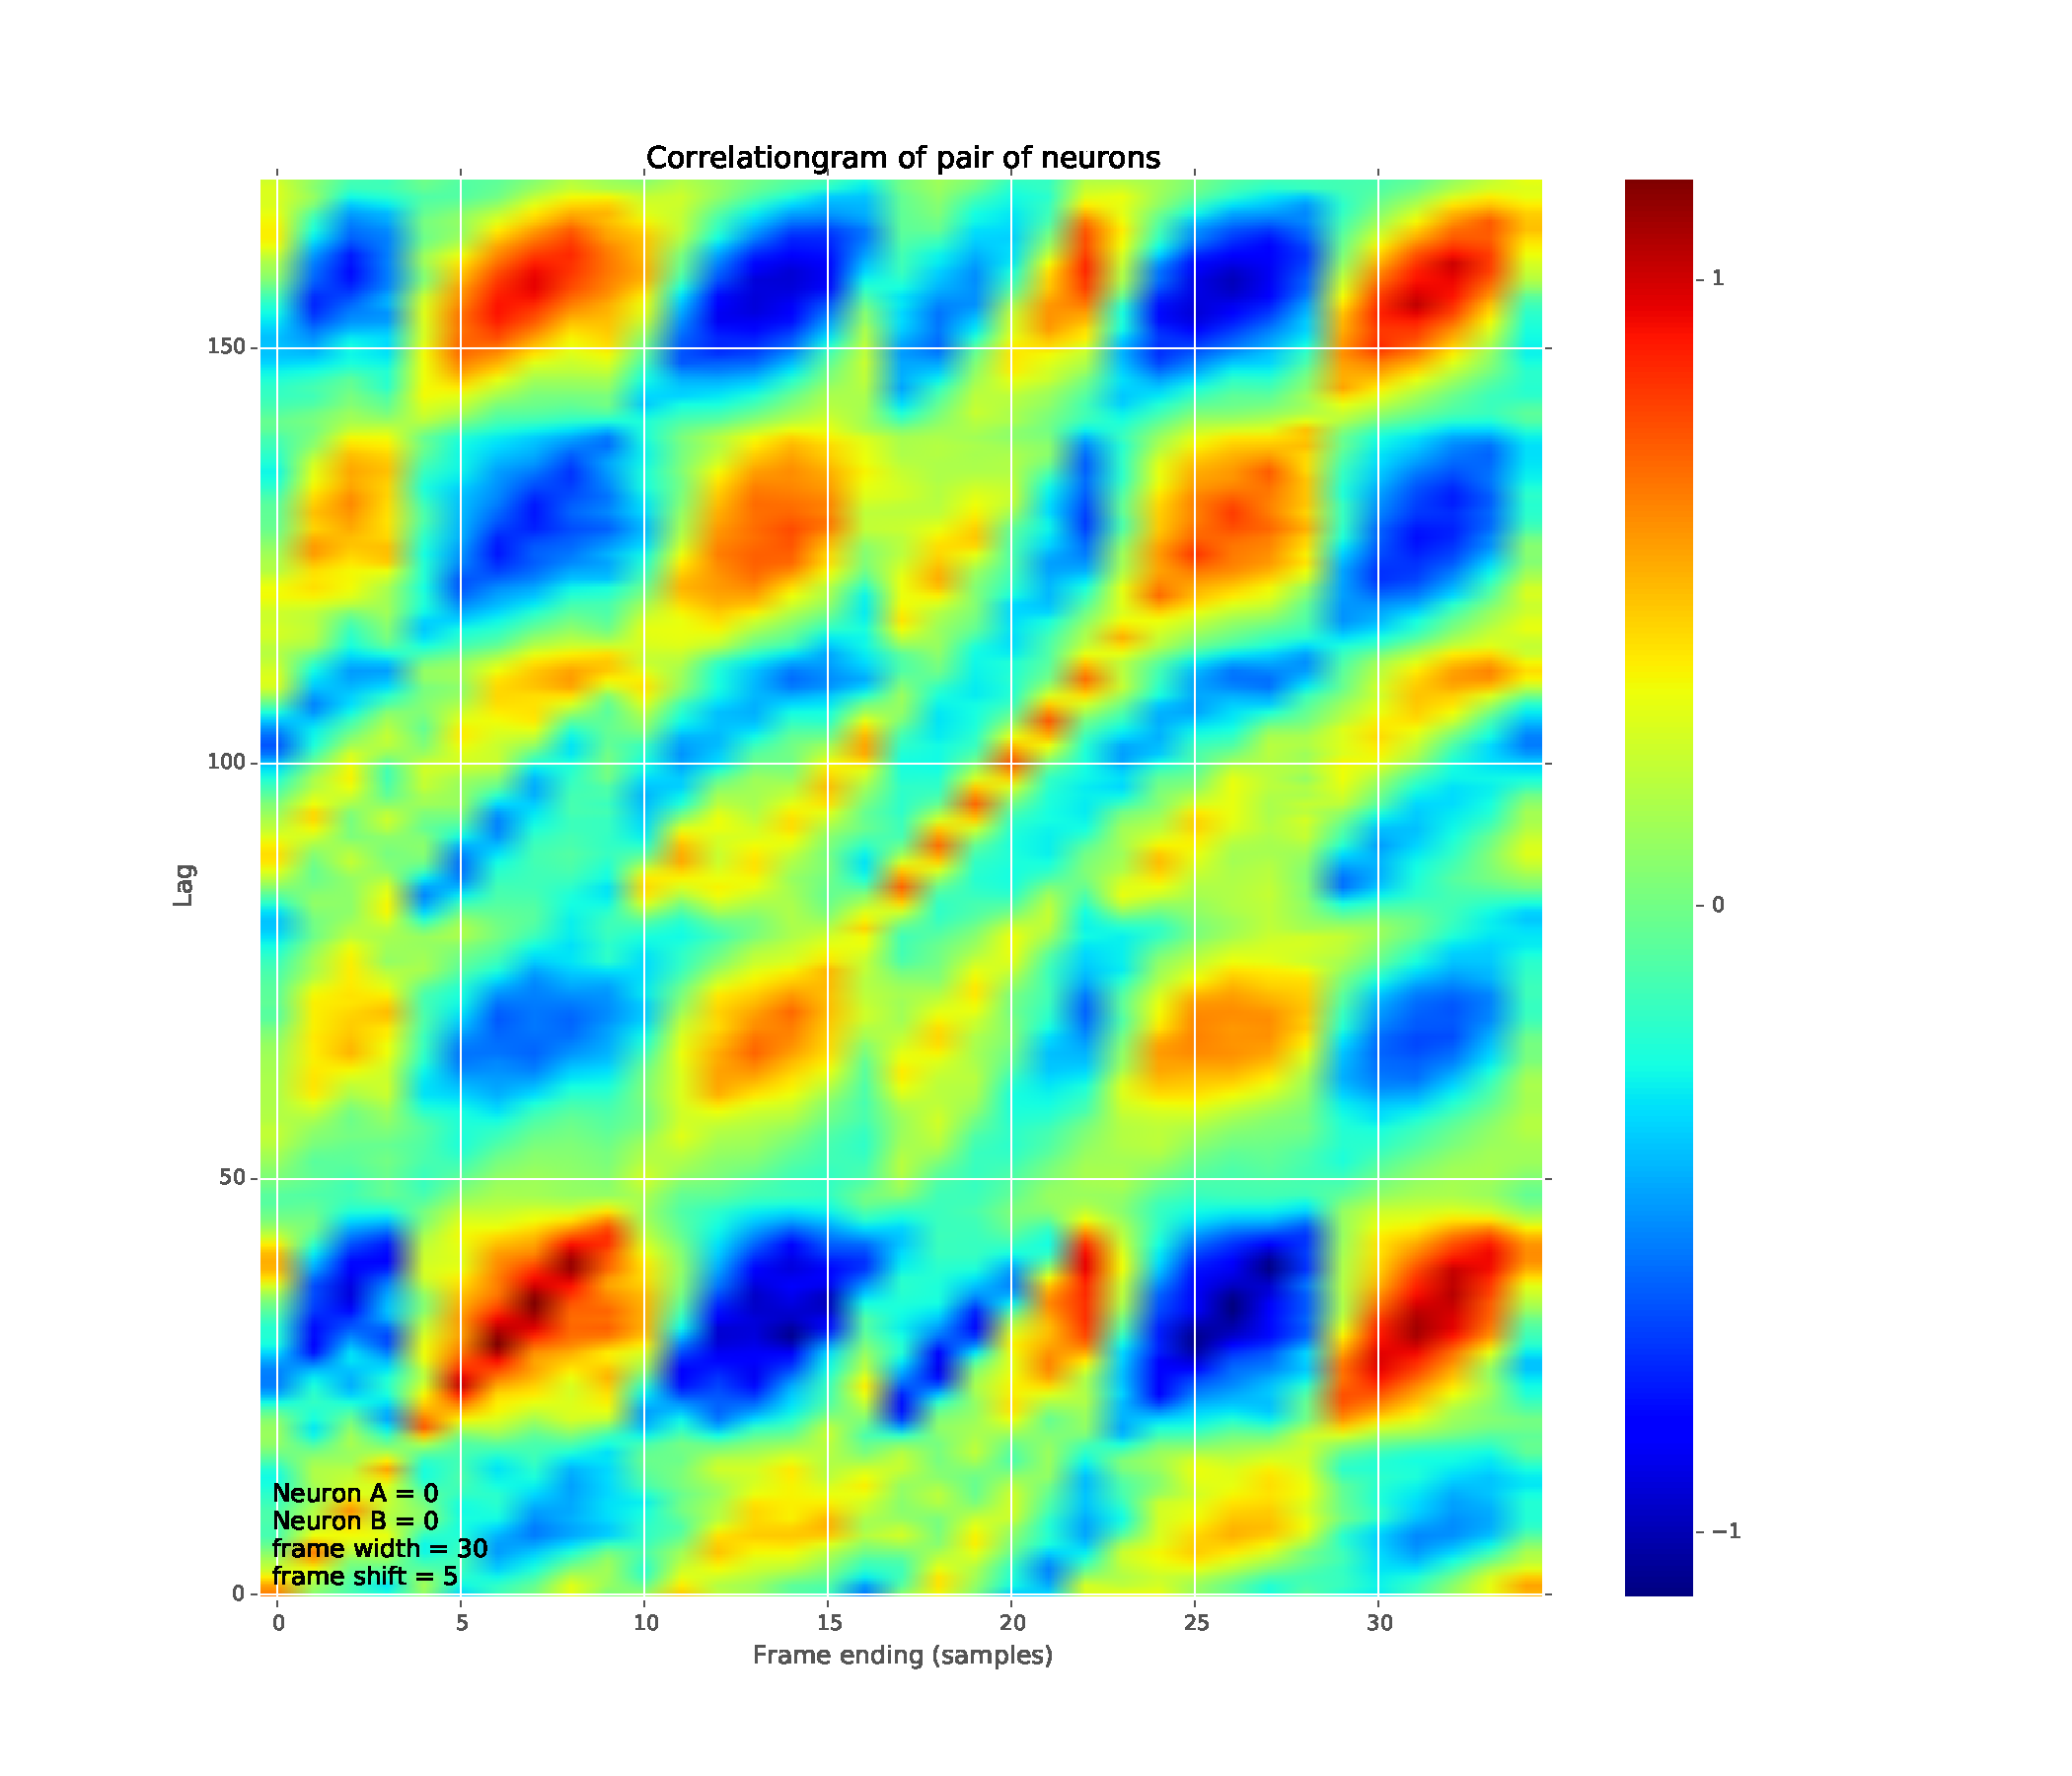
\includegraphics[width=\linewidth]{\plt/acfMain_corrGram_2016_02_05_16_49_10.pdf}
    \caption{Frame width = 30}
    \label{fig:acfgram_same}
  \end{subfigure}%
  \caption{ACFGram plots for template and target responses from same neuron.}\label{fig:oridir_simple}
\end{figure}
The Figure~\ref{fig:acfgram_diff} shows ACFGram plots for two different neuron responses. Motifs across neurons are studied for finding a better correlation metric. For different frame widths, Cross-Correlation function indicate presence of motifs across neurons. The approximate length of motifs is more than 45 samples, which is significant. Importantly, more or less any pair of neurons taken from the sampled set of 65 neurons from each mouse exhibited presence of motifs. This indicates existence of inter neuronal correlations. This supports the claim that information in V1 is coded in population by inter-neuronal correlations.
\begin{figure}[h]
  \begin{subfigure}[b]{0.5\textwidth}
    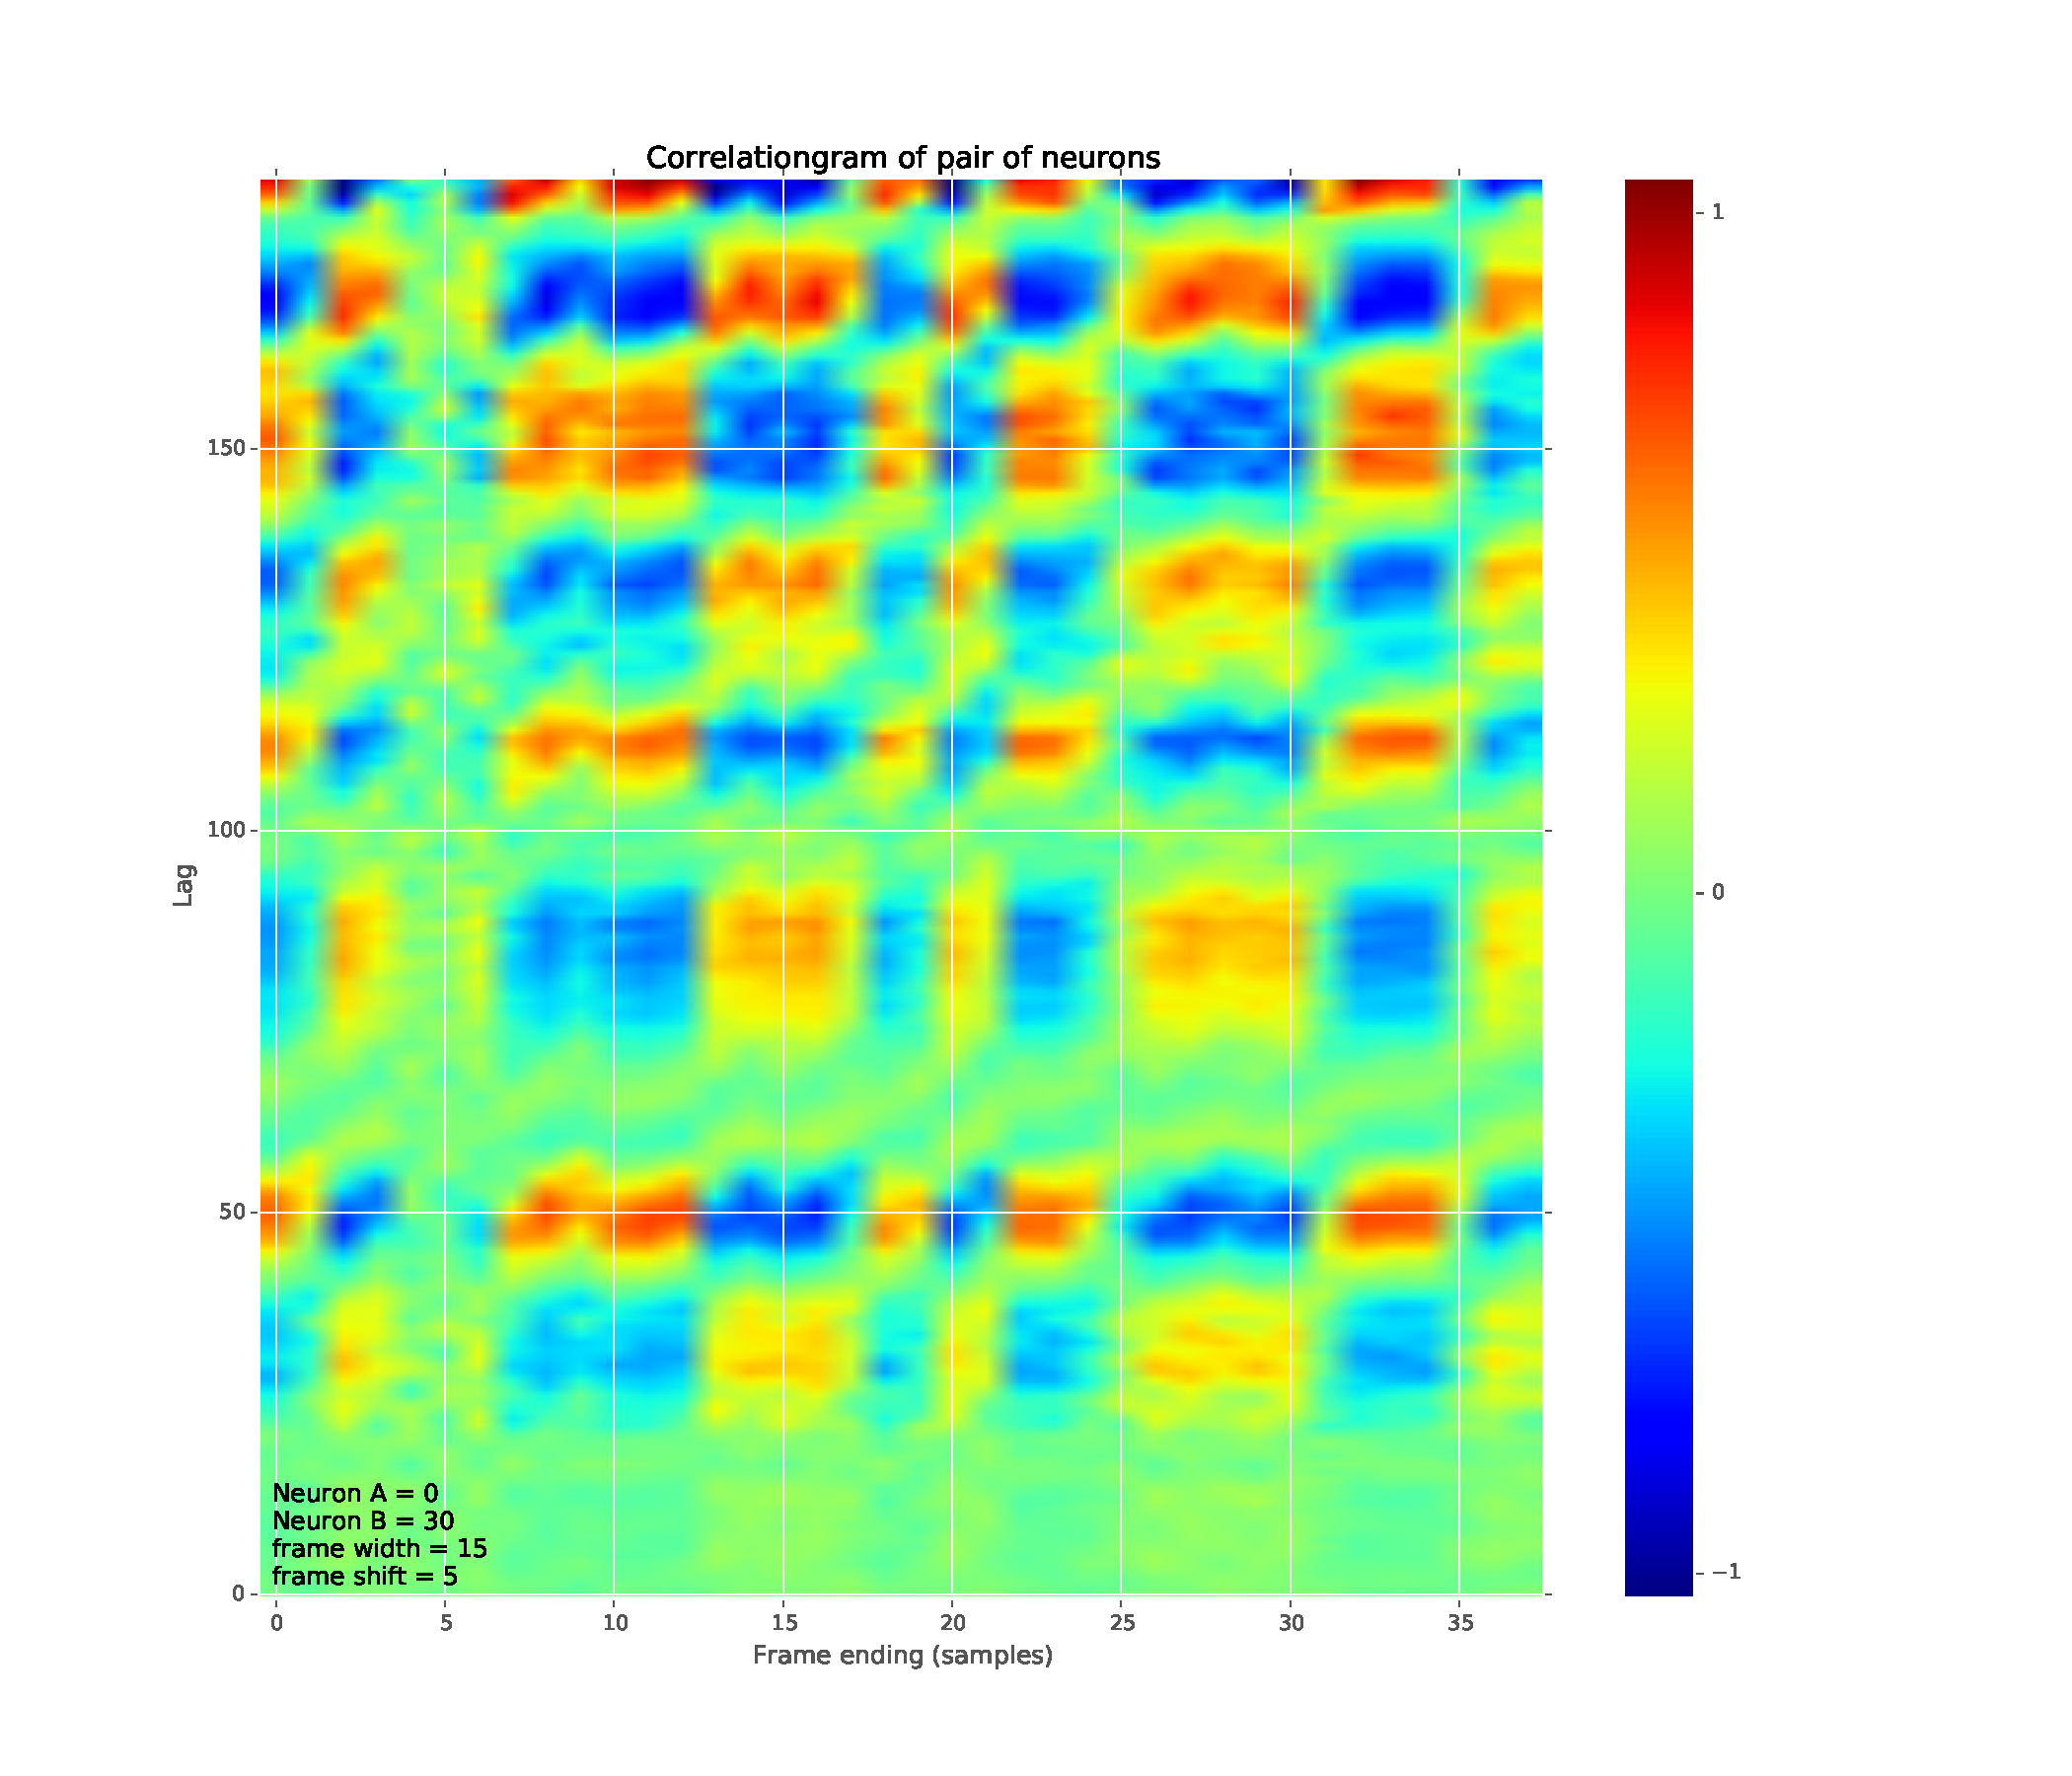
\includegraphics[width=\linewidth]{\plt/acfMain_corrGram_2016_02_05_16_45_22.pdf}
    \caption{Frame width = 15, frame shift = 5}
    \label{fig:ori_simple}
  \end{subfigure}%
  \begin{subfigure}[b]{0.5\textwidth}
    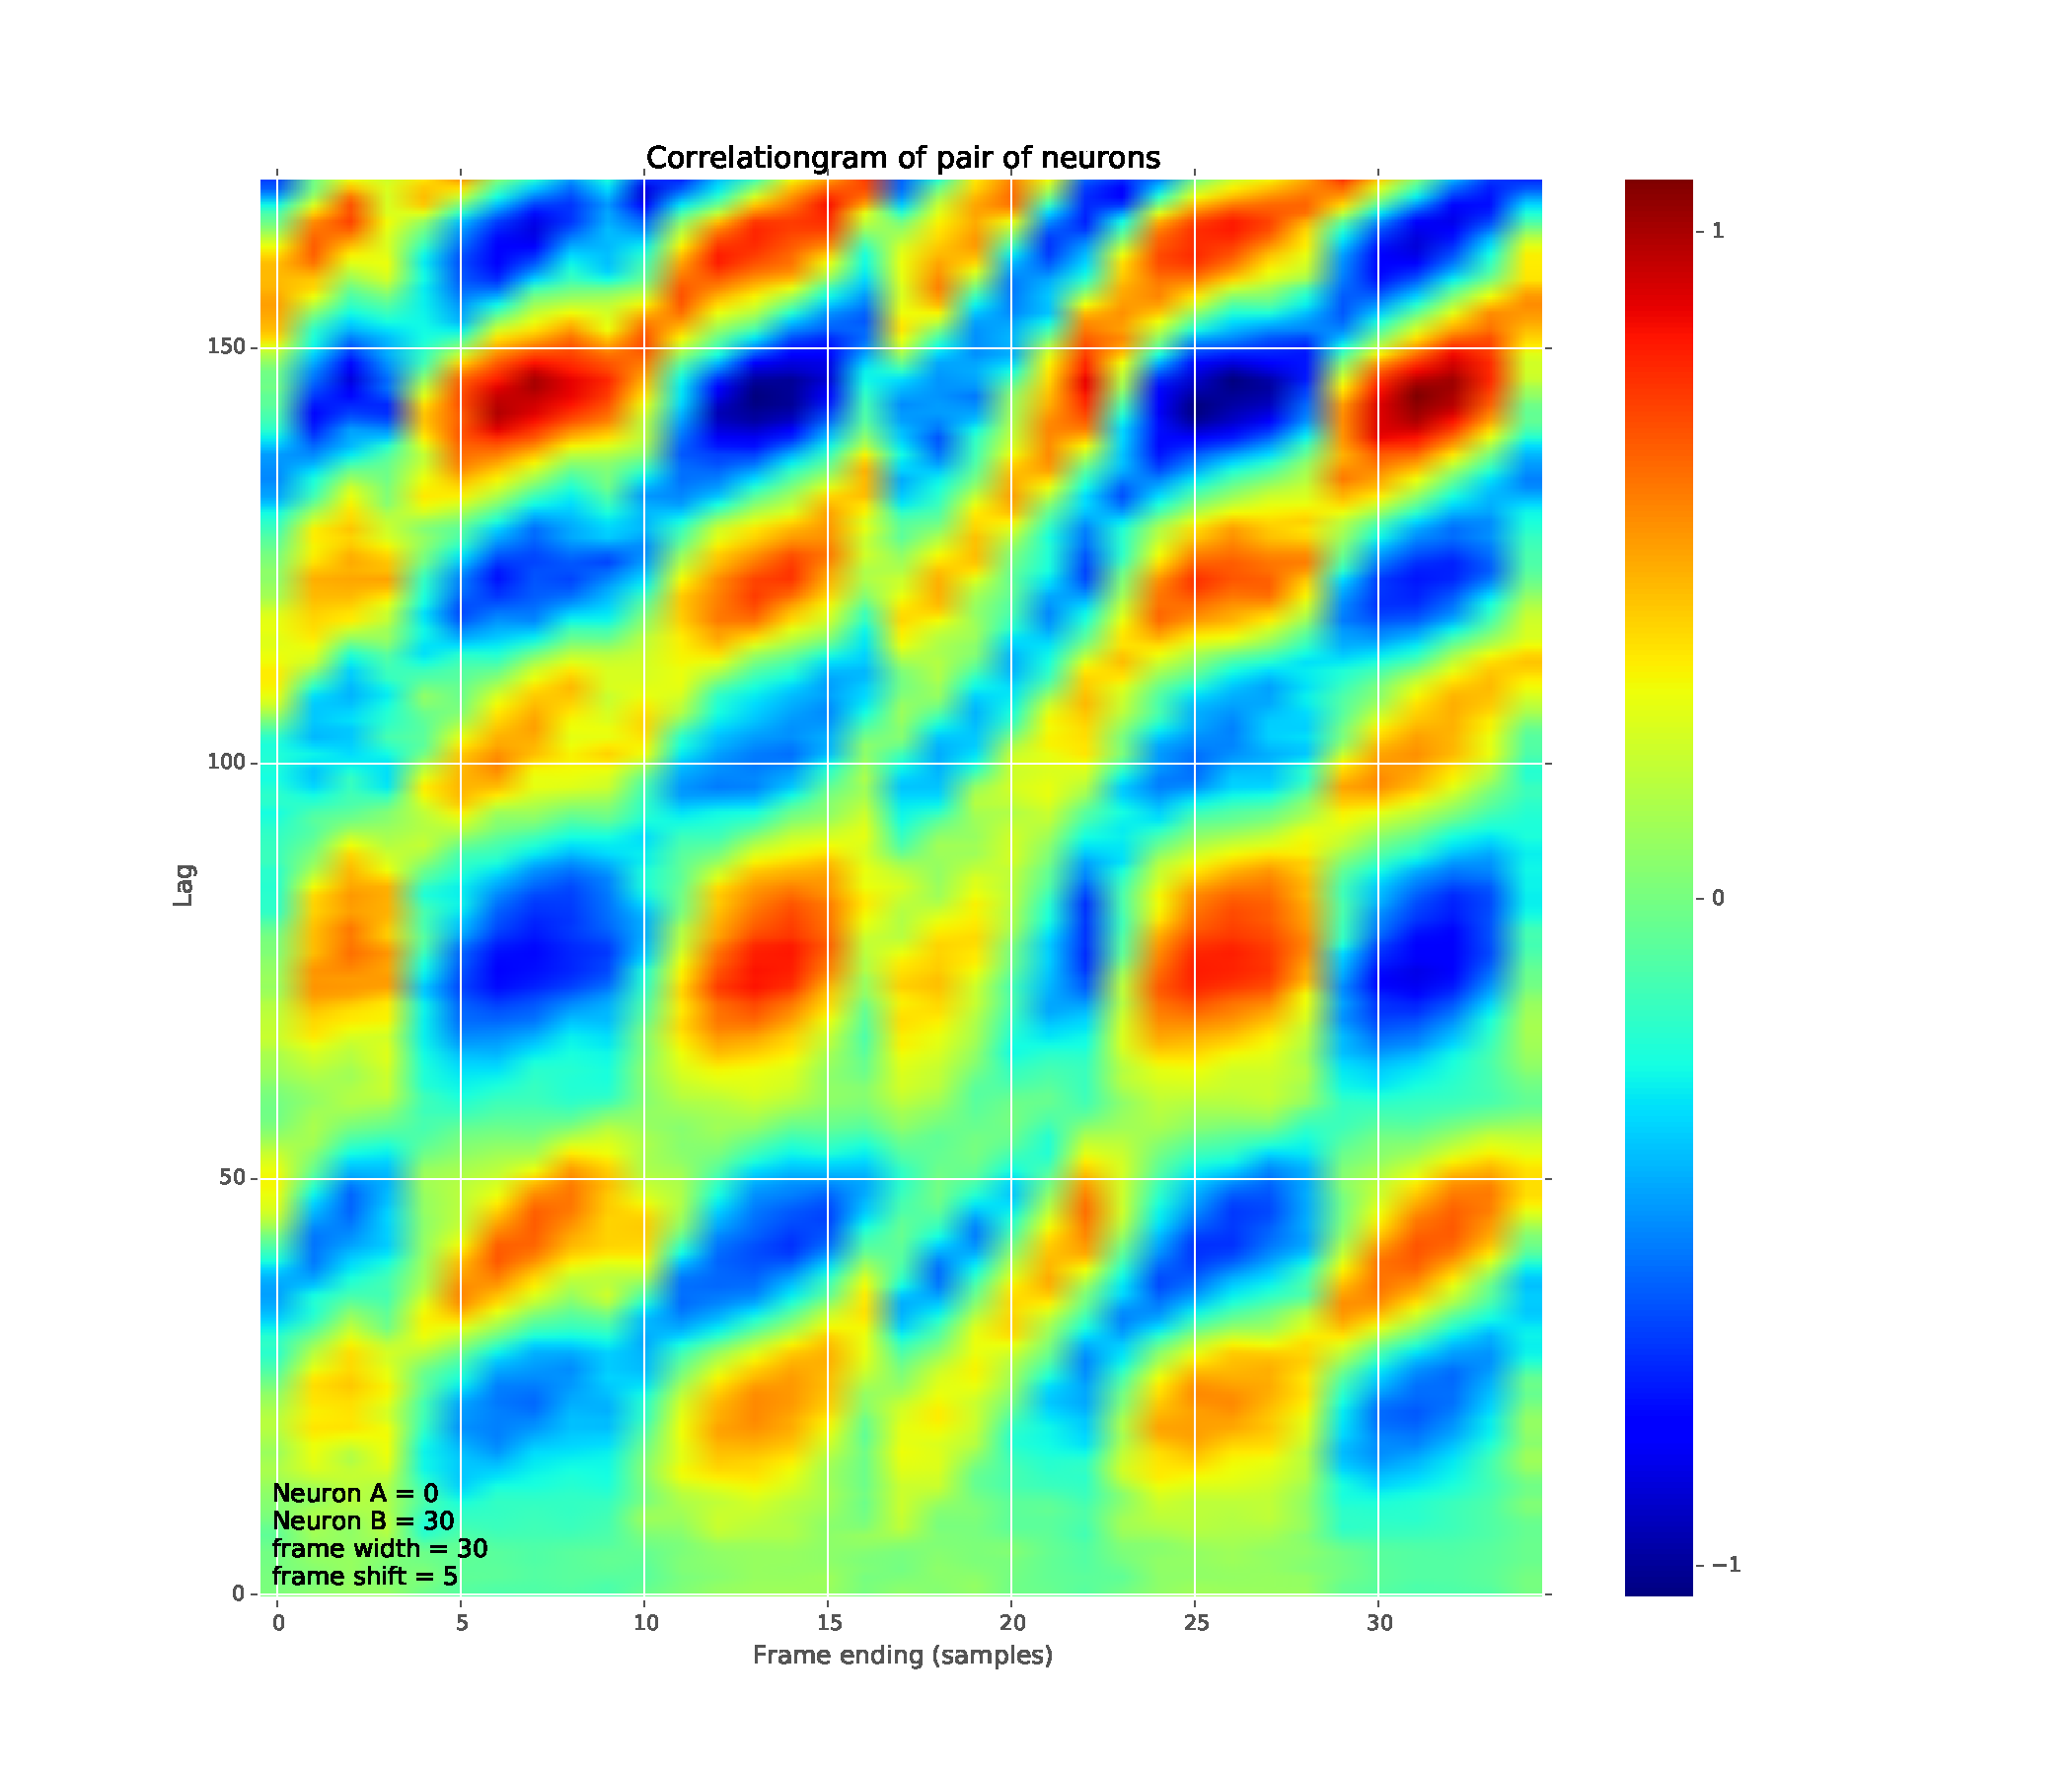
\includegraphics[width=\linewidth]{\plt/acfMain_corrGram_2016_02_05_16_45_38.pdf}
    \caption{Frame width = 30, frame shift = 5}
    \label{fig:acfgram_diff}
  \end{subfigure}%
  \caption{ACFGram plots for template and target responses from different neurons.}\label{fig:oridir_simple}
\end{figure}
The search for the presence of motifs in primary visual cortex succeeded with experimentally verifying rough common subsequences of significance ($>2$ seconds) exists in neuronal responses. This motivates us to find the longest motifs you can find between two neurons. Also till now we used Pearson correlation as a measure of similarity. We look into rough measures of similarity and longest common subsequence in the next chapter.

% section acfgram (end)

%%%%%%%%%%%%%%%%%%%%%%%%%%%%%%%%%%%%%%%%%%%%%%%%%%%%%%%%%%%%%%%%%%%%%%
\chapter{Rough Longest Common Subsequence (RLCS)}     % 12 pages
\label{chap:rlcs}
Having established existence of motifs in neuronal responses, A robust algorithm to extract best possible motifs from two signals is required. As a longer motif has more significance in the context, an algorithm which produce longest common subsequence is desirable. Longest Common Subsequence (LCS) is a classical problem in query string matching, data comparison and Bio-informatics. We will eventually look into an adapted LCS problem which can be used to match real signals called Rough Longest Common Subsequence (RLCS).

\section{Longest Common Subsequence (LCS)} % (fold)
\label{sec:longest_common_subsequence_}
A subsequence of a string $S$ is a set of characters that appear from left to right in original string $S$ but not necessarily consecutive. There will be more than one subsequence for any string with length greater than unity. For two strings $S_1$ and $S_2$, the common entries in sets of substrings of each strings are called common subsequences of $S_1$ and $S_2$. Among the common subsequences, the subsequence with maximal length is called Longest Common Subsequence. 

Some examples of LCS are given in Table~\ref{table:lcs_ex}. Note that there can be more than one LCS for a pair of strings.
\begin{table}[h]
\centering
\begin{tabular}{|c | c| c|}
\hline
String 1 - $S_1$ & String 2 - $S_2$ & LCS($S_1, S_2$) \\
\hline
ABCDGH & AEDFHR & ADH \\
AGGTAB & GXTXAYB & GTAB \\
AGCAT  & GAC     & AC, GC and GA \\
BACDB & BDCB & BCB \\
\hline 
\end{tabular}
\caption{Some examples of LCS in string comparison}
\label{table:lcs_ex}
\end{table}

LCS problem can be defined formally for two subsequences $X = (x1, x2...xm)$ and $Y = (y1, y2...yn)$ as 
$$
LCS\left(X_{i},Y_{j}\right) =
\begin{cases}
  \empty
& \mbox{ if }\ i = 0 \mbox{ or }  j = 0 \\
  \textrm{  } LCS\left(X_{i-1},Y_{j-1}\right) \frown x_{i}
& \mbox{ if } x_i = y_j \\
  \mbox{longest}\left(LCS\left(X_{i},Y_{j-1}\right),LCS\left(X_{i-1},Y_{j}\right)\right)
& \mbox{ if } x_i \ne y_j \\
\end{cases}
$$

Where $X_i = (x1, x2...xi)$ and $Y_j = (y1, y2...yj)$.

LCS problem has an optimal substructure- the problem can be broken down into subproblems of similar kind. As the problem also has overlapping subproblems, thus a Dynamic Programming approach is used to find the LCS. Running time of the dynamic programming approach is  $O(nm)$ where n and m are the lengths of strings.
% section longest_common_subsequence_ (end)

\section{RLCS} % (fold)
\label{sec:rlcs}
LCS problem can be adapted for signal matching. Instead of equality, a rough distance measure is used. If the distance between samples is less than a threshold, they are considered a match. It is not desirable just to optimize the length of subsequence in signals as the gaps between selected samples can cause false alarms. Dynamic Programming algorithm for rough signal matching has to be penalizing gaps and motivating matches. The rest of the problem and the solution remains similar to LCS problem and similar Dynamic Programming approach can solve the problem efficiently.

Modified LCS problem with rough comparison is stated below. The RLCS of two discreet signal sequences $X = <x1, x2...xm>$ and $Y = <y1, y2...yn>$ is obtained by maximizing the score value $S$.
$$
S\left(X_{i},Y_{j}\right) =
\begin{cases}
  0
& \mbox{ if }\ i = 0 \mbox{ or }  j = 0 \\
  \textrm{  } S\left(X_{i-1},Y_{j-1}\right) \frown x_{i}
& \mbox{ if } dist(x_i , y_j) < \tau_{dist} \\
  \mbox{max}\left(S\left(X_{i},Y_{j-1}\right),S\left(X_{i-1},Y_{j}\right)\right)
& \mbox{ if } dist(x_i , y_j) > \tau_{dist} \\
\end{cases}
$$
Where $X_i = <x1, x2...xi>$ and $Y_j = <y1, y2...yj>$.

Various context uses different distance measures for comparing samples.  Manhattan distance (city block distance) of notes is used in work [\cite{lin2011music}] in the context of music matching. In a work on verification of Raga in Carnatic music [\cite{duttaraga}], a domain specific similarity measure is used. RLCS on neuronal signals in this work uses normalized Euclidean distance for comparing similarity.
$$dist(x_i, y_i) = (x_i - y_j)^2$$
Distances are normalized from 0 to 1 by performing: 
$$dist(x_i, y_i) = \frac{dist(x_i, y_i) - minDist}{maxDist - minDist}$$
Where $minDist$ is the minimum pairwise distance and $maxDist$ is the maximum pairwise distance.

Most important part of RLCS is the adapted score update rules. In the classical LCS problem, the gaps between the a common subsequence is not penalized; Instead only the length of the subsequence was of consideration. But in signals, having a gap in between will give a poor match of signal. So it is important to penalize the gaps and reward matches.
The following score update rules penalizes gaps in subsequence and awards positive score for matches.
\begin{enumerate}
  \item Score update for a match. $dist(x_i, y_j) < \tau_{dist}$\\
  $$score(i, j) = score(i - 1, j - 1) + 1 - \frac{dist(x_i, y_j)}{\tau_{dist}}$$
  This case happens when a match is found. The score should be rewarded with a positive value.  The maximum awarded score is 1 for an exact sample match and minimum score of 0 is given when the distance equals distance threshold ($dist(j, j) = \tau_{dist}$)threshold. The closer the samples, more the score; Lesser the gap between samples, more the score.
  \item Score update for a mismatch. $dist(x_i, y_j) > \tau_{dist}$\\
  $$score(i, j) = score(i - 1, j - 1) - \delta$$
  We allowed any number of gaps in a string LCS problem. But in the case of signals, we cannot allow large gaps as it would produce false alarms. We penalize each mismatching samples with a constant score $\delta$.
\end{enumerate}
The problem is then recursively solved using  Dynamic Programming algorithm which will provide us with a 2-D score matrix. The Dynamic programming algorithm for input sequences $X = <x_0, x_1, ..., x_{m-1}>$ and $Y = <y_0, y_1, ..., y_{n-1}>$ is explained in algorithm ~\ref{rlcs_algo}.

\begin{algorithm}
\caption{Dynamic Programming algorithm for RLCS}
\label{rlcs_algo}
\begin{algorithmic}[1]
  \Function{RLCS}{X, Y, $\tau_{dist}$, $\delta$}
    \State $p \gets min(m, n)$
    \For {$i = 0$; $i < m$; $i++$}
      \For {$j = 0$; $j < n$; $j++$}
        \State $dist(i, j) \gets euclideanDistance(x_i, y_j)$
      \EndFor
    \EndFor
    \State $\text{minDist} \gets min(dist)$ \Comment{For normalization}
    \State $\text{maxDist} \gets min(dist)$ \Comment{For normalization}\\

    \State $c\gets zeros(m+2, n+2)$ \Comment{For storing running score}
    \State $s \gets zeros(m+2, n+2)$ \Comment{For storing score}
    \State $d \gets zeros(m+2, n+2)$ \Comment{For backtracking}
    \State $p \gets zeros(m+2, n+2)$ \Comment{For storing partial scores.}\\

    \For {$i = 0$; $i < m$; $i++$}
    \For {$j = 0$; $j < n$; $j++$}
      \State $d \gets (dist(i, j) - \text{minDist})/(\text{maxDist} - \text{minDist})$ 
      \Comment{Normalize}
      \If {($d < \tau{dist}$)} 
        \State $d (i, j) \gets ` \nearrow '$\Comment{Path to travel while backtracking}
        \State $c (i, j) \gets c (i-1, j-1) + (1 - d/\tau_{dist})$
        \State $s (i, j) \gets s (i-1, j-1)$
      \ElsIf {$c (i-1, j) > c (i, j-1)$}
        \State $d (i, j) \gets ` \uparrow'$
        \State $c (i, j) \gets c (i-1, j) - \delta$\Comment{Penalize}
        \State $c (i, j) \gets max(0, c (i, j))$
        \If {($d (i-1, j) == `\nearrow')$}
            \State $s(i, j) \gets (p (i-1, j)*p^2 + (c (i-1, j)/p)^2$
        \Else
            \State $s (i, j) \gets s (i-1, j)$
        \EndIf
      \Else
        \State $d (i, j) \gets ` \leftarrow'$
        \State $c (i, j) \gets c (i, j - 1) - \delta$\Comment{Penalize}
        \State $c (i, j) \gets max(0, c (i, j))$
        \If {($d (i, j - 1) == `\nearrow')$}
            \State $s(i, j) \gets (p (i, j - 1)*p^2 + (c (i, j - 1)/p)^2$
        \Else
            \State $s (i, j) \gets s (i, j - 1)$
        \EndIf        
      \EndIf
    \EndFor
  \EndFor
  \State \Return $c, s, d, p$
  \EndFunction
\end{algorithmic}
\end{algorithm}

Backtracking through score matrix will gives the Longest Common Subsequence. As we have been penalizing gaps, there will be points in the track where score is zero. For each sample match increases and for every mismatch, score decreases. So the zero in backtracking path will mean that there are enough mismatches to balance the total positive score created by matches. This identifies the boundary of a common subsequence. A number of subsequences could be extracted by cutting backtrack path at points where score is zero. This set of subsequences are called \textbf{Longest Common Subsequence Set} (LCSS) [\cite{duttaraga}]. Algorithm~\ref{backtrack_algo} explains backtracking to extract the LCSS.

\begin{algorithm}
\caption{Backtracking to find the subsequences}
\label{backtrack_algo}
\begin{algorithmic}[1]
  \Function{backtrack}{X, Y, c, s, d}
    \State $\text{maxScore} \gets max(s(i, j))$
    \State $ x, y \gets indexOf(\text{maxScore})$
    \State $l \gets 0$
    \While {$(x \ne 0)$ and $(y \ne 0)$}
        \State $\text{segment} (l) = [x - 1, y - 1, c (x, y) ]$
        \State $l = l + 1$
        \If {$(d (x, y) == `\nearrow')$}
            \State $x = x + 1$
            \State $y = y + 1$
        \ElsIf {$(d (x, y) == `\uparrow')$}
            \State $x = x + 1$
        \Else
            \State $y = y + 1$
        \EndIf
    \EndWhile
  \EndFunction
\end{algorithmic}
\end{algorithm}
\subsection{Motivic analysis of Neuronal signals with RLCS} % (fold)
\label{sub:motivic_analysis_of_neuronal_signals_with_rlcs}
Having established presence of motifs in neuronal responses, we use Rough Longest Common Subsequence (RLCS) algorithm to find the `best' motifs from neuronal responses. Penalizing the gaps makes RLCS a good signal matching algorithm.

The experiments are conducted on responses of neurons from V1 of 11 mice to different visual stimuli. Each signal is sampled at 20 Hz and last for 10 seconds. The study is split into different sections based on which neurons the signals for analysis come from.
\subsubsection{Motifs in responses of a neuron to different trials} % (fold)
\label{ssub:motifs_in_responses_of_a_neuron_to_different_trials}
The signals from a neuron's response to different trials of same stimuli are passed to RLCS algorithm to detect motifs. The Figure~\ref{img:score_trial} shows score matrix obtained after RLCS. The effect of $\tau_{dist}$ was experimentally studied and fixed at $0.005$. For $\tau_{dist}$ above $0.001$, number of false alarms increased. Decreasing threshold further caused bad detection rate. The desired motif takes a path through the score matrix. The diagonal shifts in the score path are sample matches - as a result of that we can see the increase in score. Shifting to right or top denotes a gap in the subsequence. As mismatches cause penalty, the score will decrease. When enough mismatches to compensate the total positive score are encountered, The score will become zero. Such points on the backtrack path having zero score mark boundaries of subsequences.
\begin{figure}[h]
    \centering
    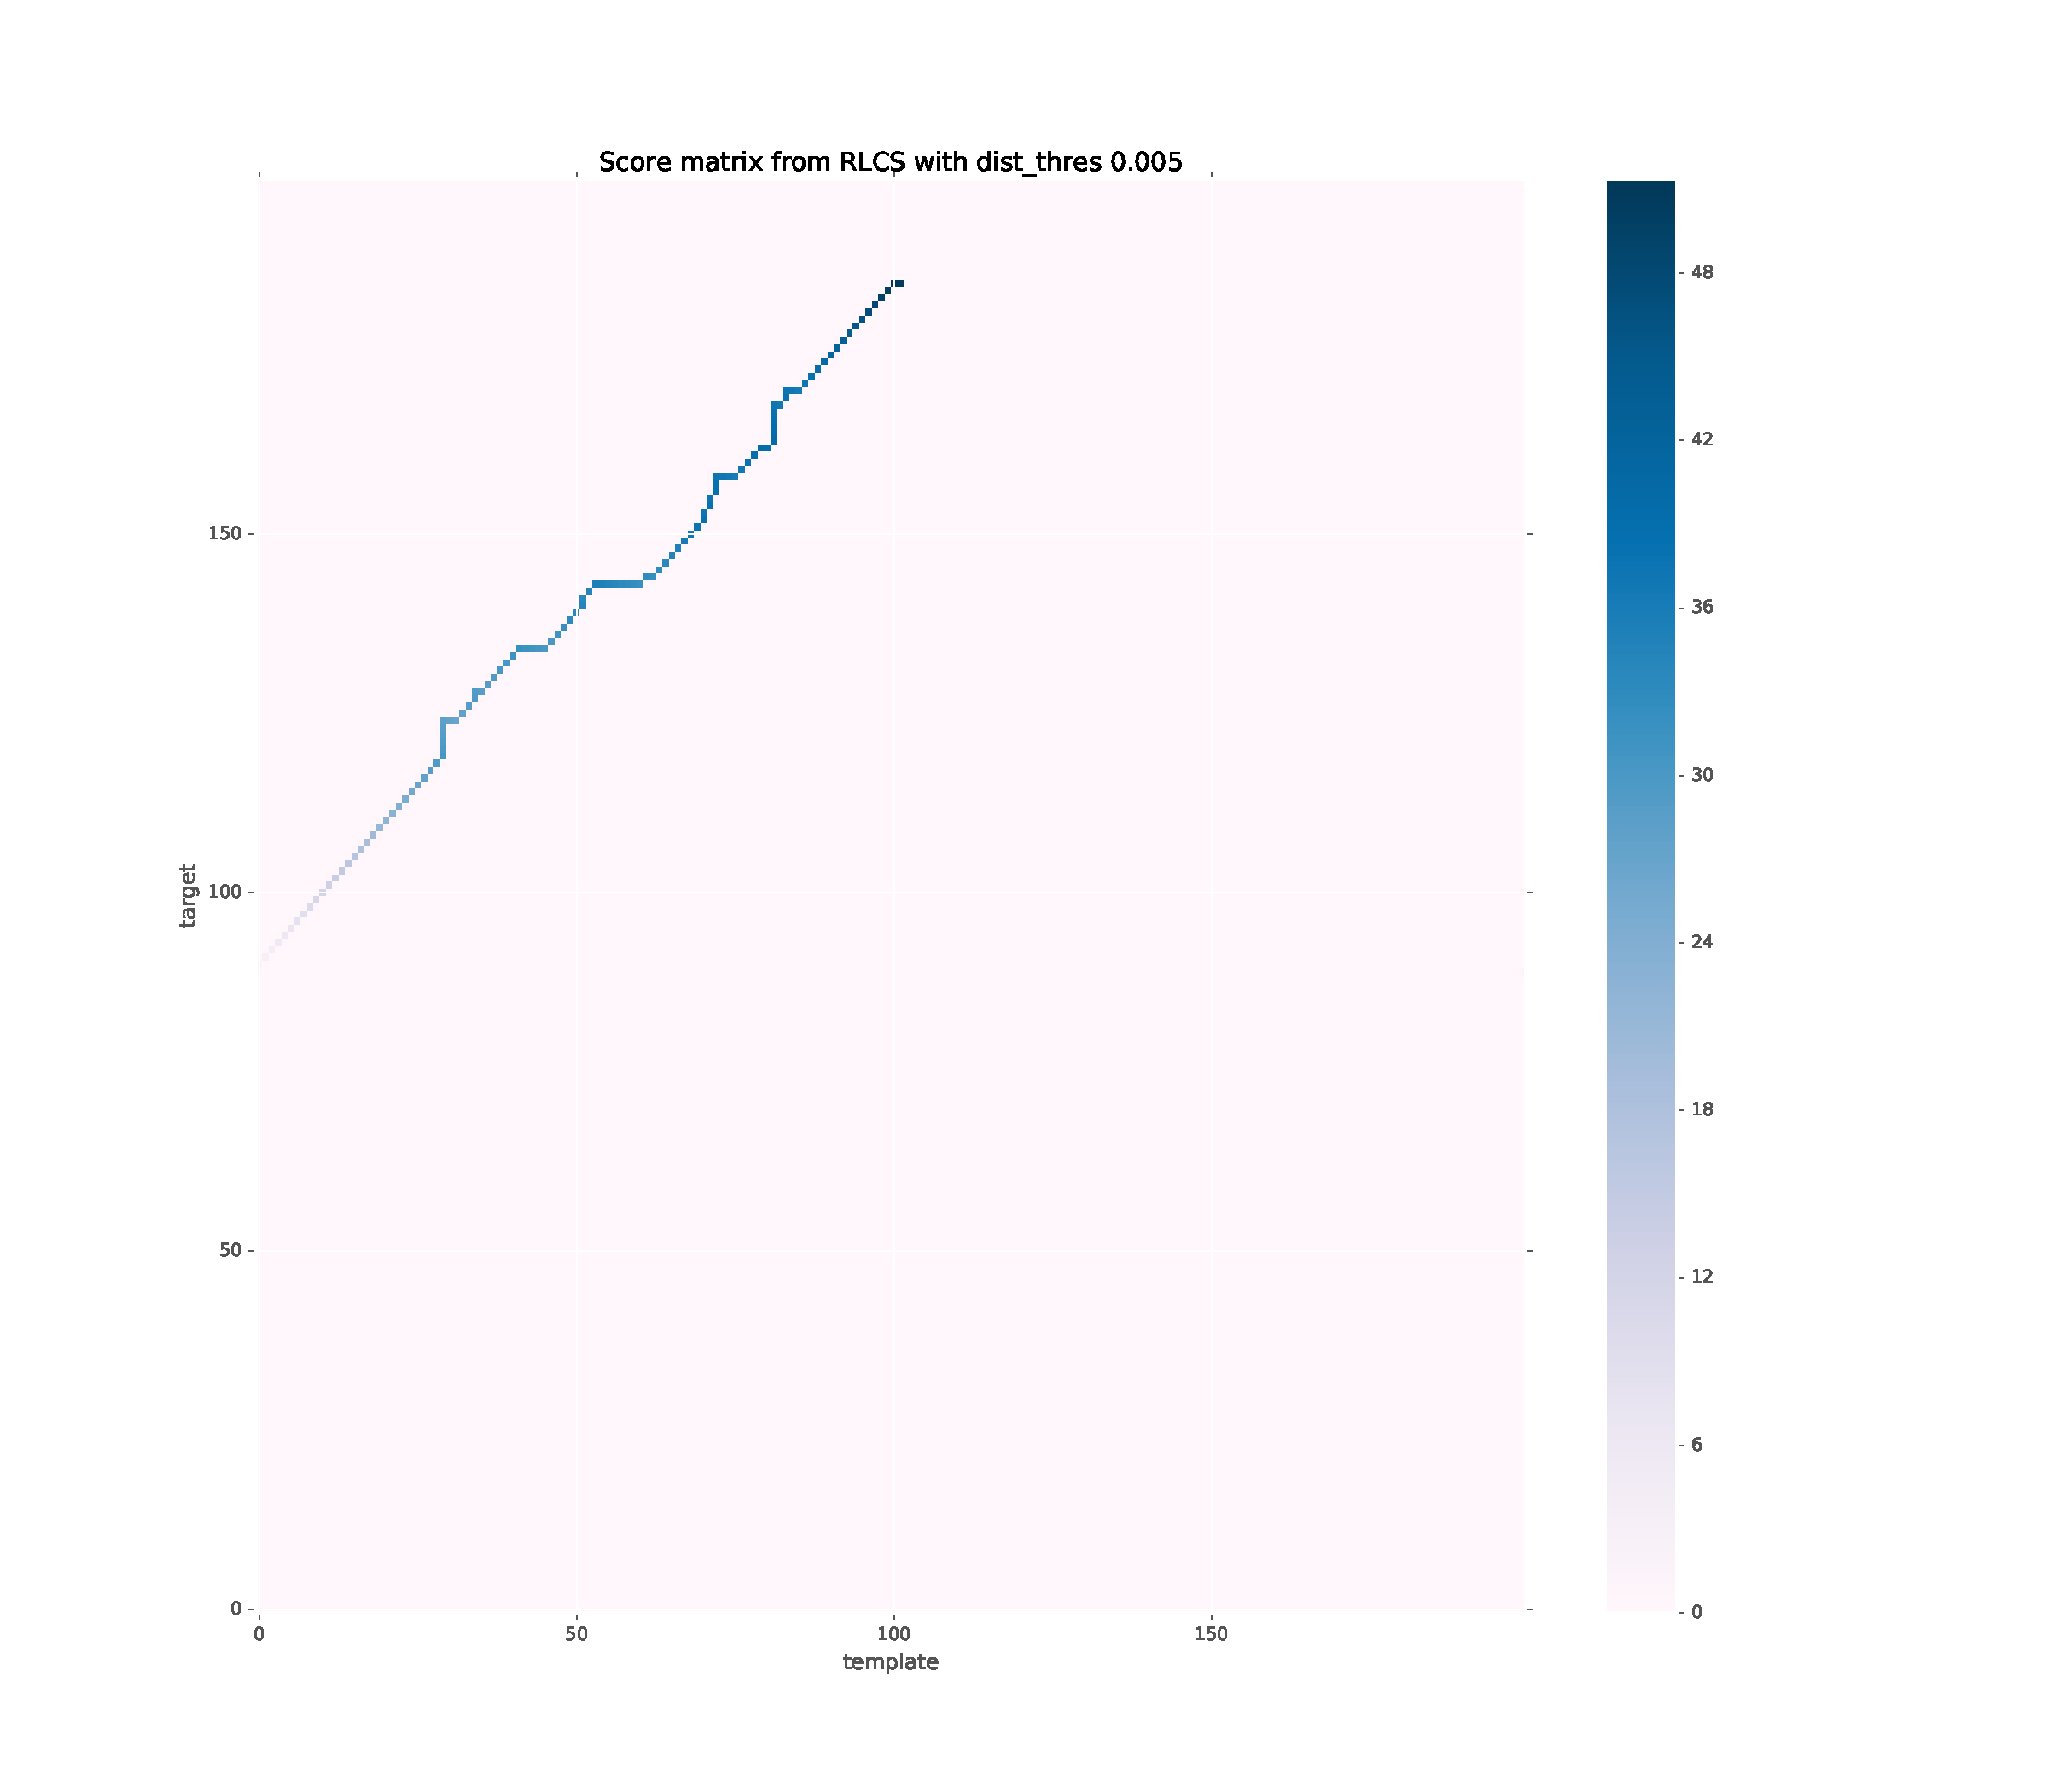
\includegraphics[width=\linewidth]{\plt/rlcsMain_score_trial_0_1n_102016_05_06_10_32_05.pdf}
    \caption{Score matrix from RLCS of responses a neuron to different trials.}
    \label{img:score_trial}
\end{figure}

The Figure~\ref{img:motif_trial} shows a motif from the responses of a neuron to different trials. The signal retrieved shows good similarity. At 50Hz sampling frequency, the motif lasts more than $1.5$ seconds. Which is a significant time for two neurons to have very similar response. Also, similar phenomena occurs in each neuron we studied.
\begin{figure}[h]
    \centering
    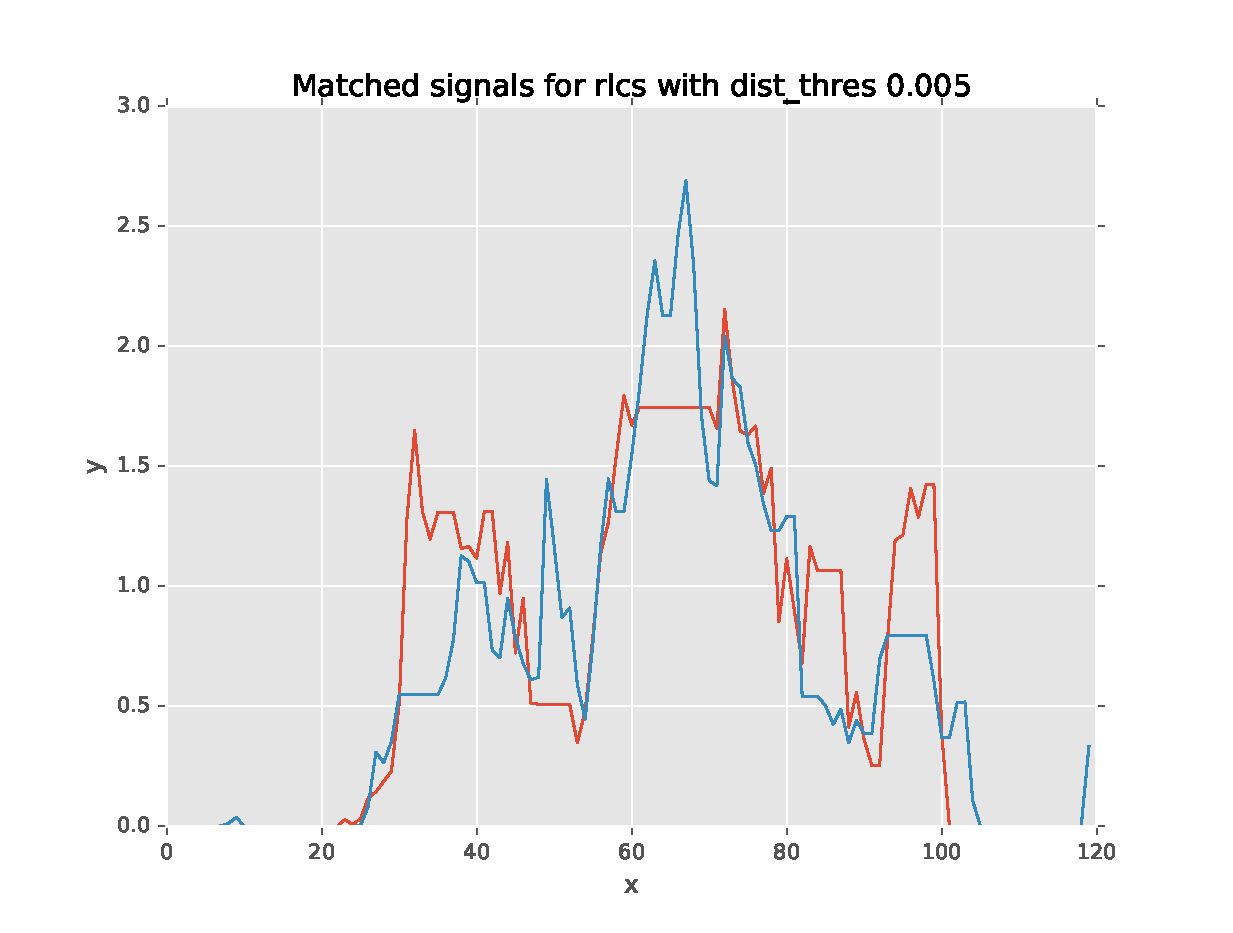
\includegraphics[width=.8\linewidth]{\plt/rlcsMain_motif_trial_0_1n_102016_05_06_10_30_17}
    \caption{Extracted motif (longest) from responses a neuron to different trials.}
    \label{img:motif_trial}
\end{figure}
% subsubsection motifs_in_responses_of_a_neuron_to_different_trials (end)
\subsubsection{Motifs in responses of two neurons in a mice} % (fold)
\label{ssub:motifs_in_responses_of_two_neurons_in_a_mice}
Responses of two neurons to same visual stimuli are analyzed for motifs. Both neurons were sampled simultaneously during experiment. The Figure~\ref{img:score_neuron} shows score matrix and Figure~\ref{img:motif_neuron} shows longest motif spotted. Note that in this case, motif has a duration of 2.5 seconds. In the score matrix, two disconnected paths can be found. Each one of these correspond to a common subsequence. Set of such subsequences is called LCSS. Motifs across mice have an average duration about $1$ seconds. More or less any two neurons taken for study, motifs of length 40 samples were spotted. This shows correlation in responses of neurons. In some cases, the length of motif exceeded $2$ seconds.
\begin{figure}
    \centering
    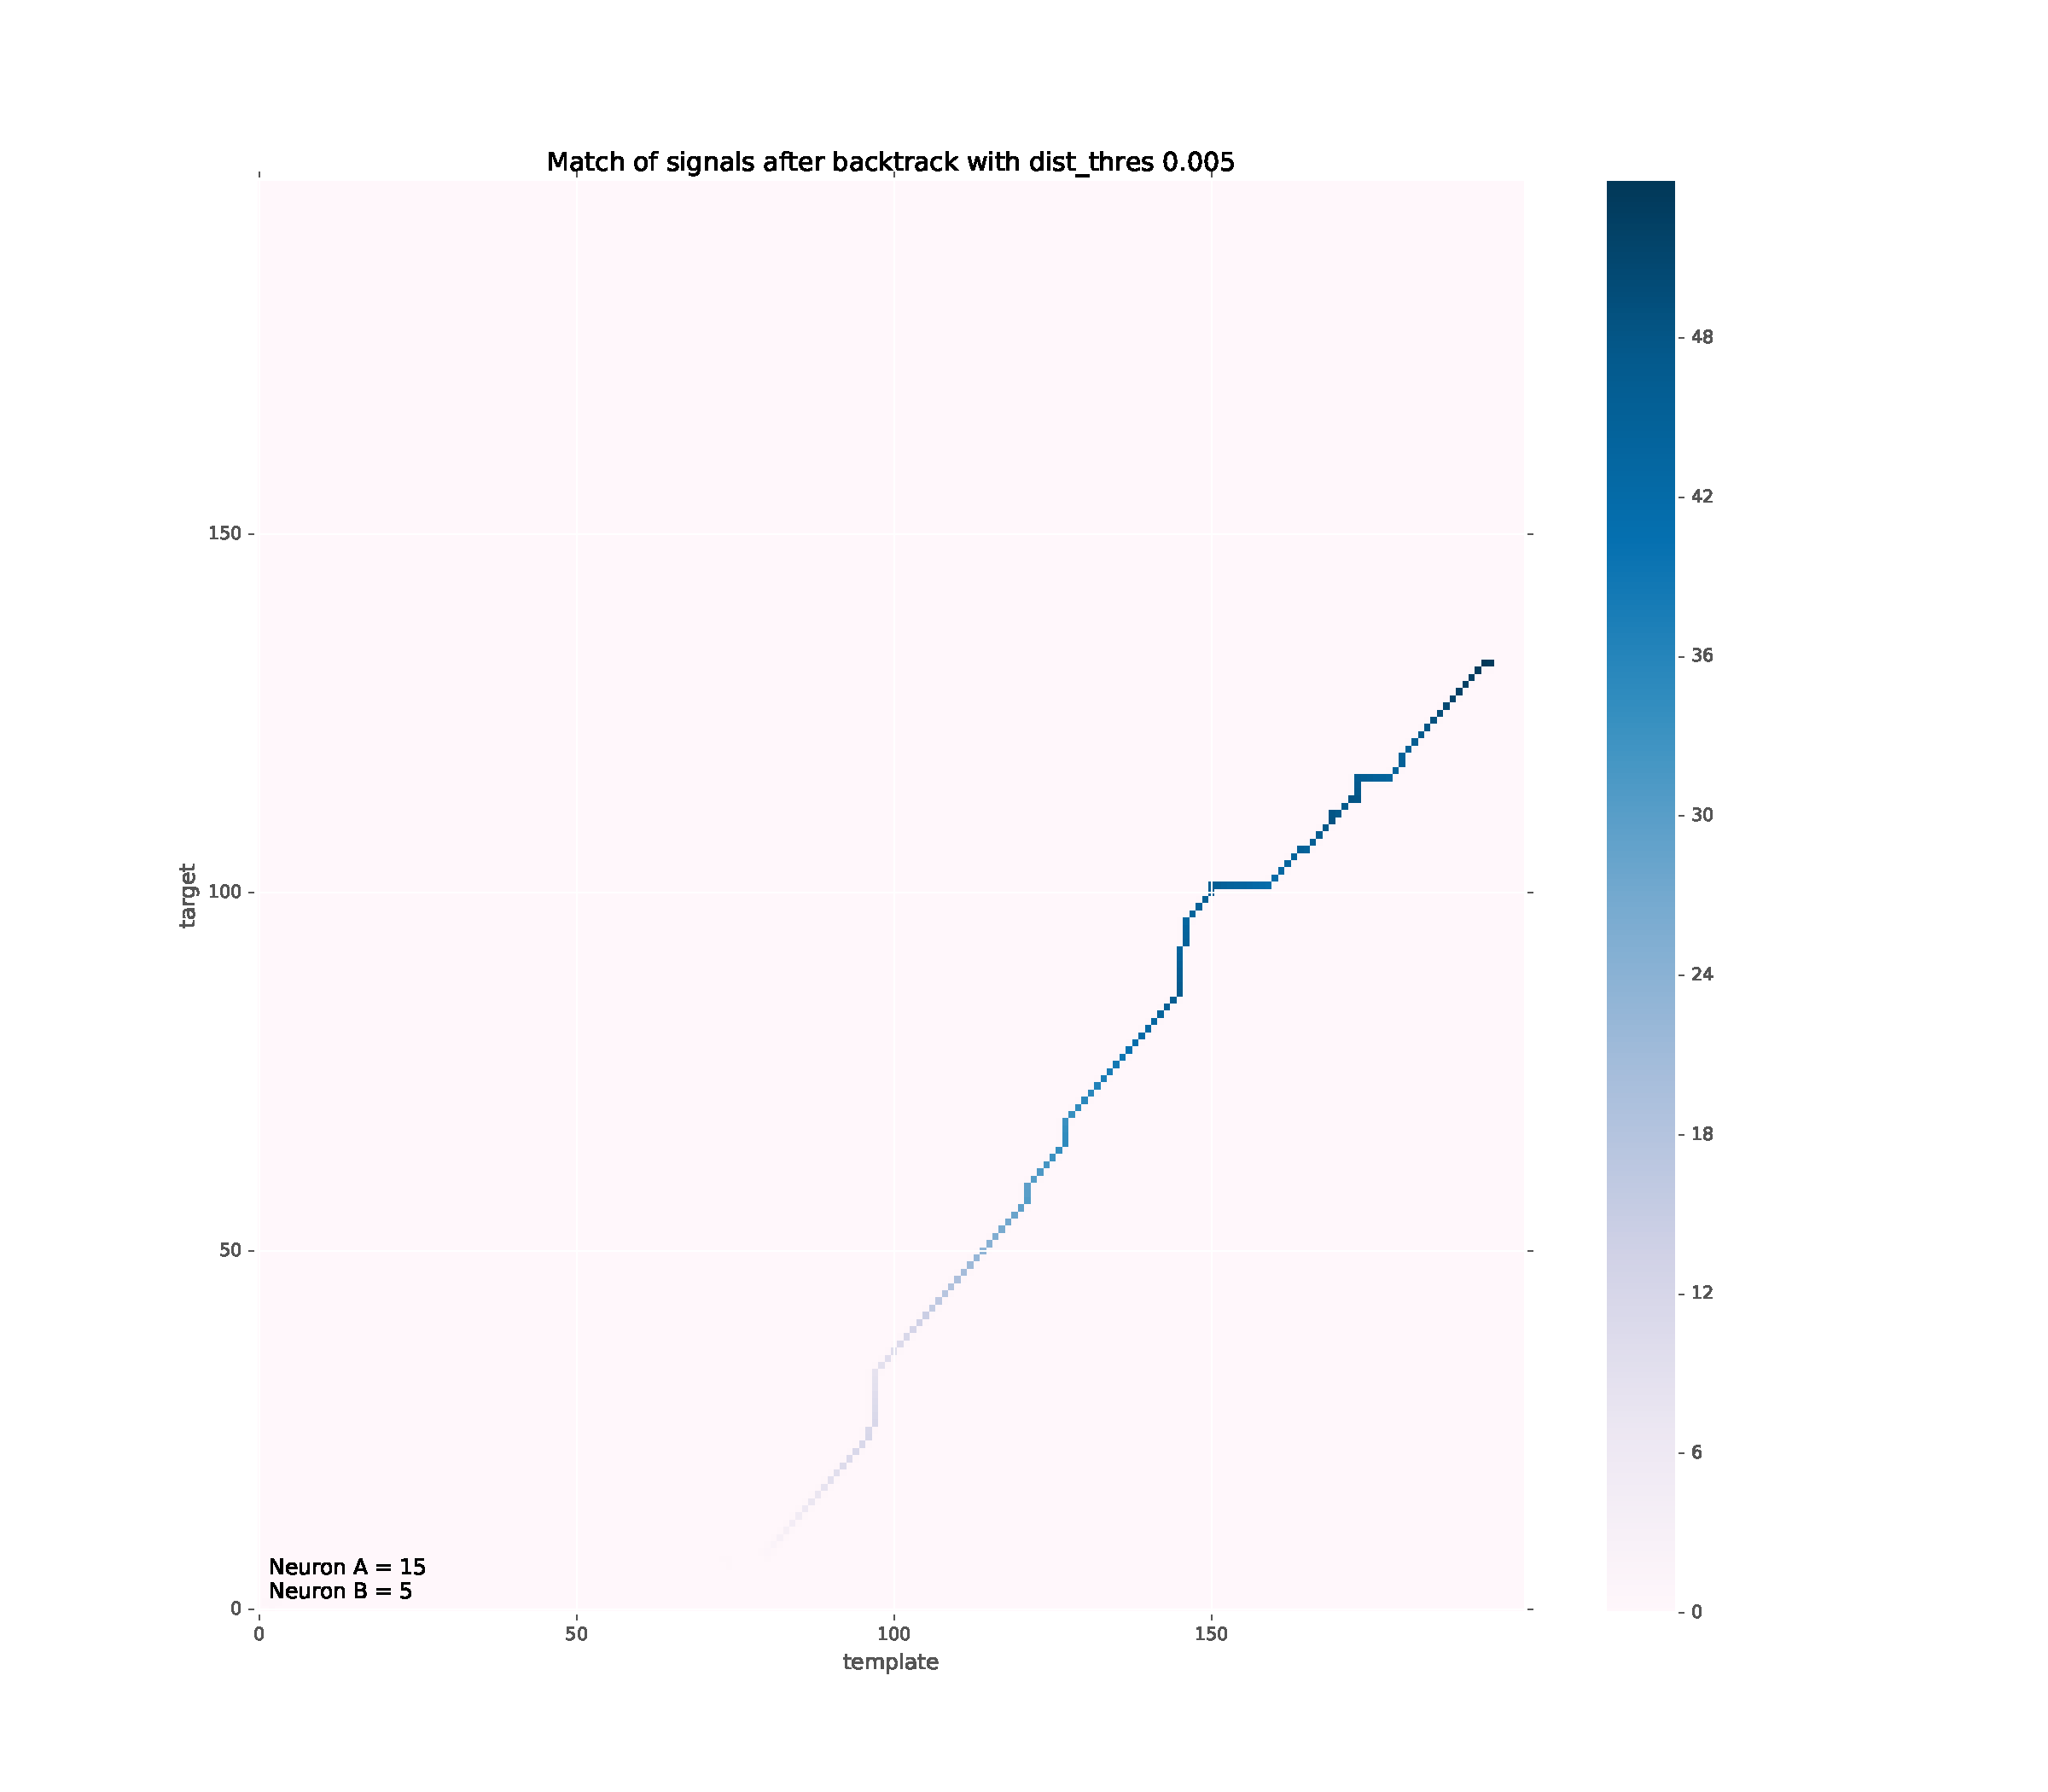
\includegraphics[width=.8\linewidth]{\plt/rlcsMain_backtrack_n1_15_n2_52016_05_06_10_42_55.pdf}
    \caption{Score matrix from RLCS of responses of two neurons in a mouse.}
    \label{img:score_neuron}
\end{figure}
\begin{figure}
    \centering
    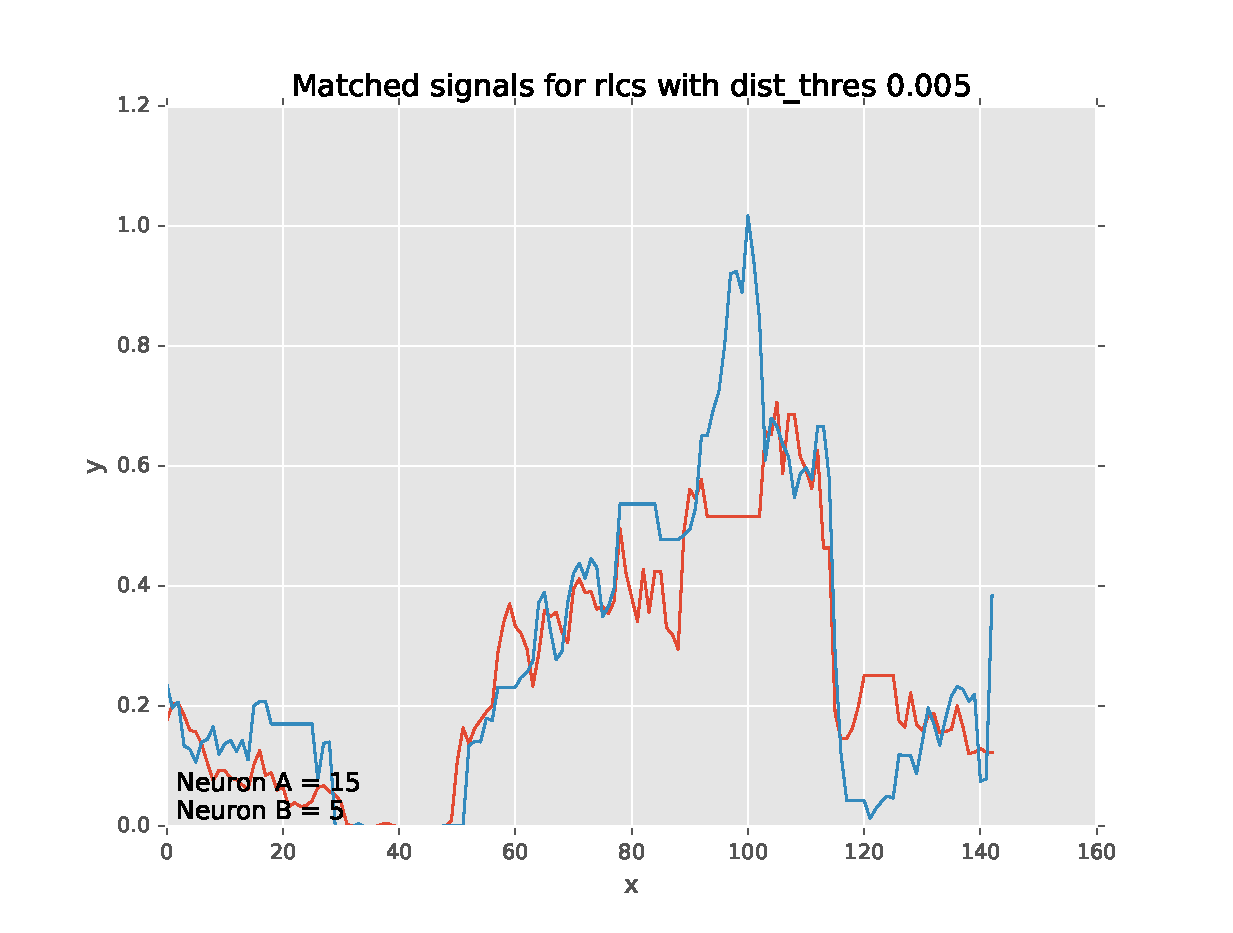
\includegraphics[width=.8\linewidth]{\plt/rlcsMain_getSegs_15_n2_52016_05_06_10_42_54}
    \caption{Extracted motif (longest) from responses of two neurons in a mouse.}
    \label{img:motif_neuron}
\end{figure}
% subsubsection motifs_in_responses_of_two_neurons_in_a_mice (end)
\subsubsection{Motifs in responses of neurons across different mice} % (fold)
\label{ssub:motifs_in_responses_of_neurons_across_different_mice}
Two neurons across two mice were taken for study. As these neurons does not have any interconnections, the motifs are expected to have less duration if at all they exists. The experimental study proved that motifs across mice occurs very less frequent than previous cases. Even when they exists, they have short duration $\sim 0.5$ seconds. Motifs across mice could be caused by similar activation mechanism of neurons. This explains absence of long motifs across mice and presence of short subsequences. Exceptionally in some cases motifs of duration $\sim 1.2$ seconds were spotted across mice. Figure~\ref{img:score_mice} and Figure~\ref{img:motif_mice} shows score matrix and extracted motif from responses of two neurons across mice. More plots of score matrix and motifs are in Appendix~\ref{chap:rlcsplots_appndx}.
\begin{figure}
    \centering
    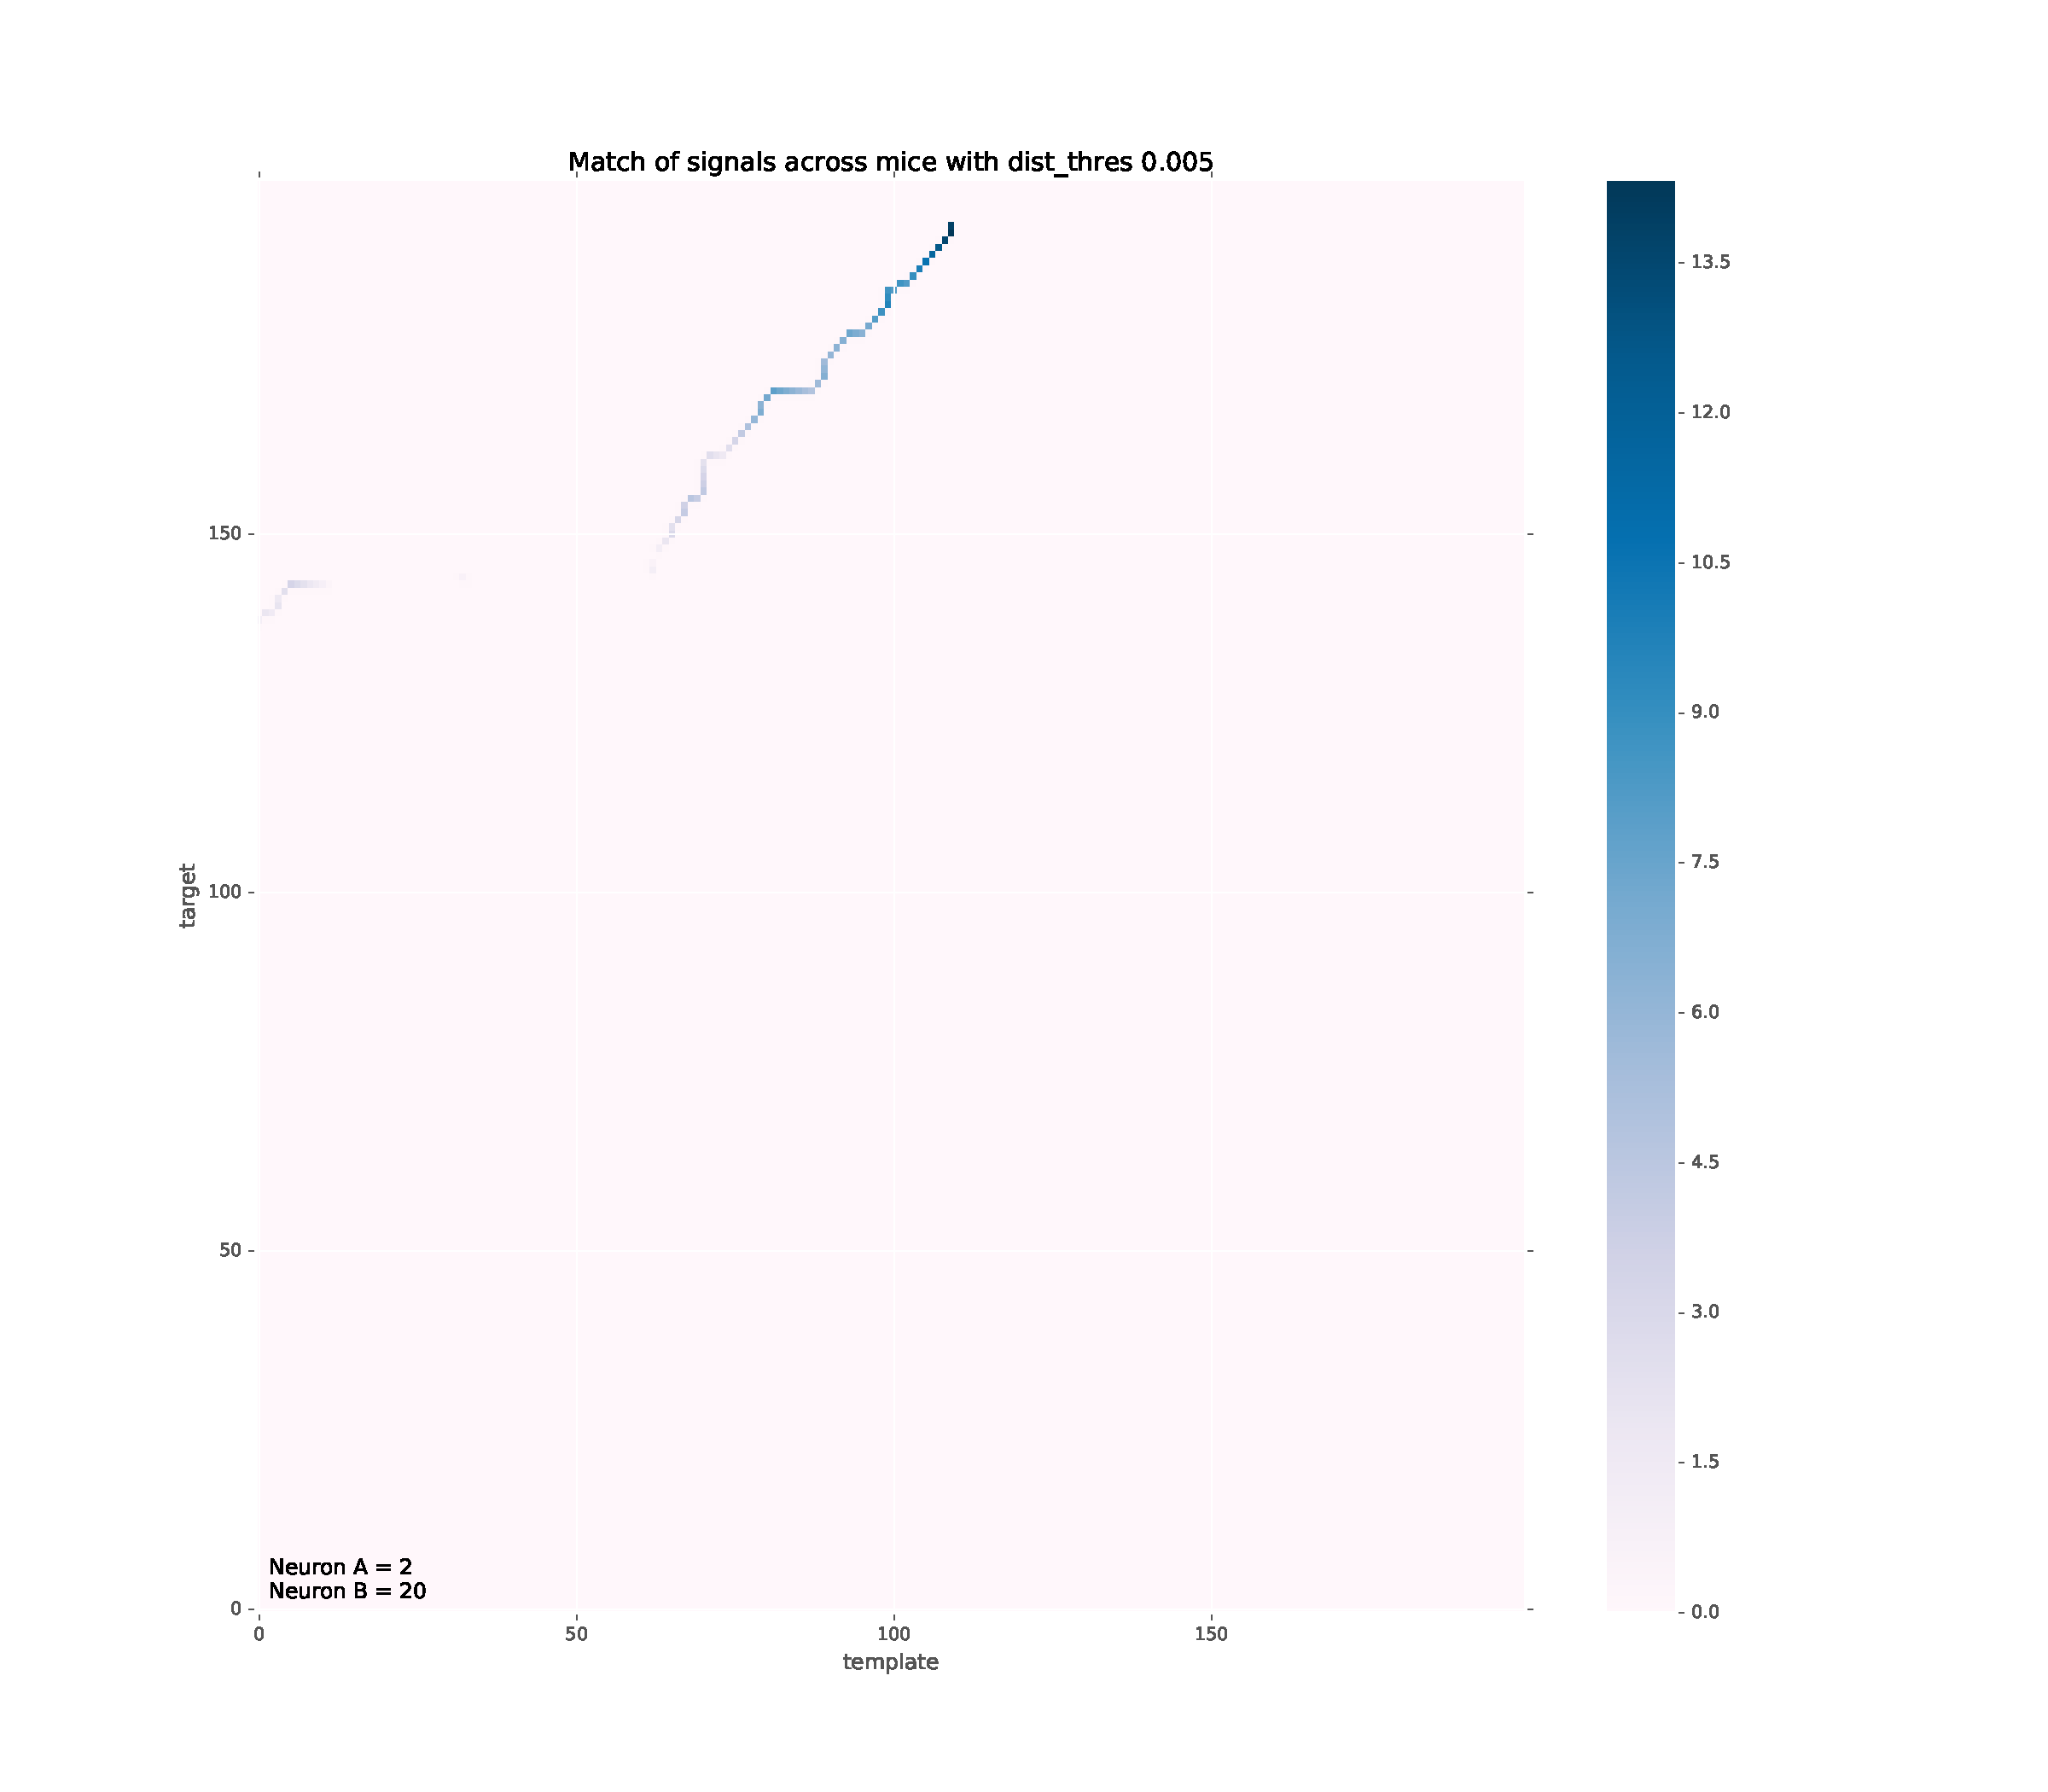
\includegraphics[width=0.8\linewidth]{\plt/rlcsMain_backtrack_mice_2016_05_06_10_48_51.pdf}
    \caption{Score matrix from RLCS of responses of two neurons in a mouse.}
    \label{img:score_mice}
\end{figure}
\begin{figure}
    \centering
    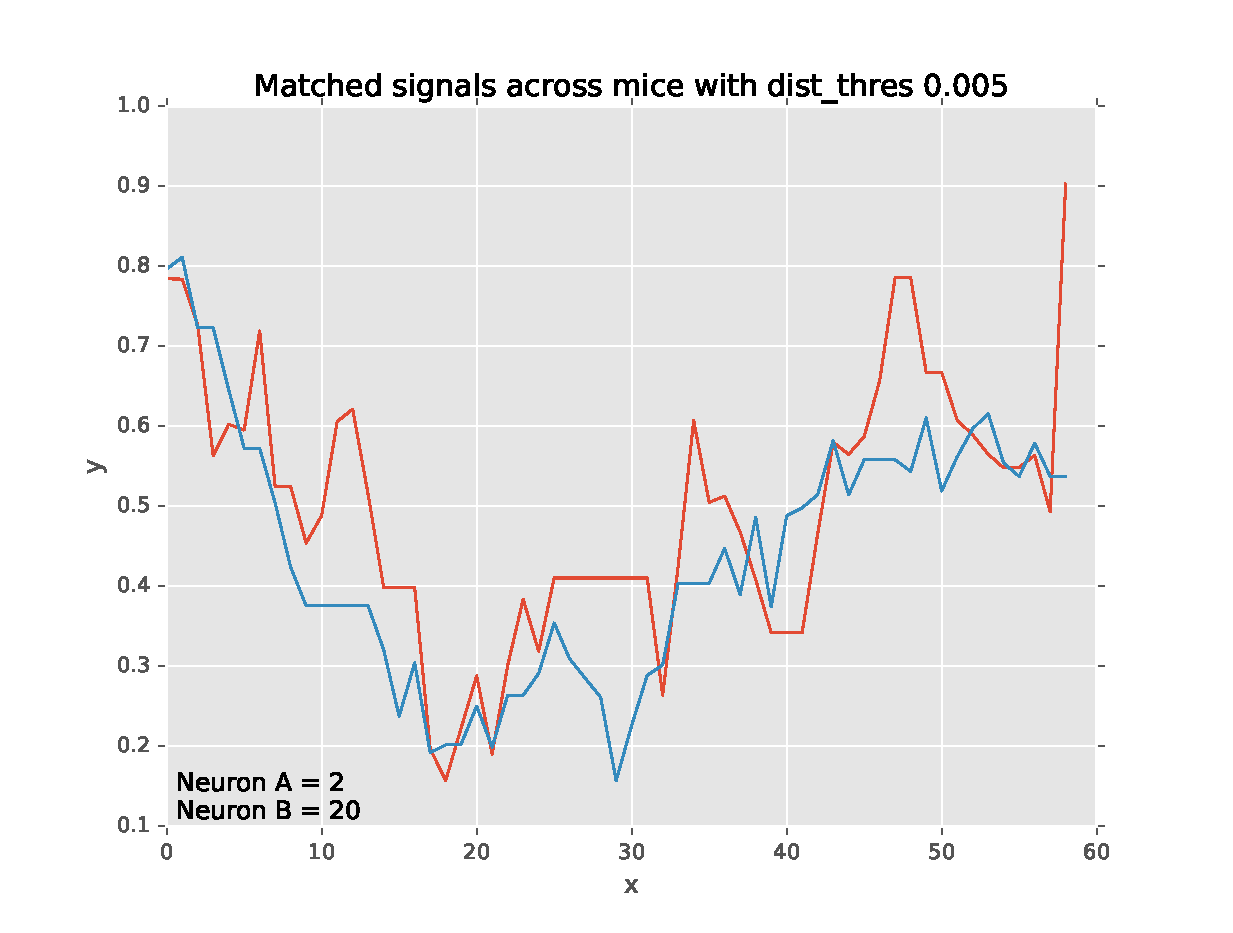
\includegraphics[width=0.8\linewidth]{\plt/rlcsMain_getSegs_mice2016_05_06_10_48_51}
    \caption{Extracted motif (longest) from responses of two neurons in a mouse.}
    \label{img:motif_mice}
\end{figure}
% subsubsection motifs_in_responses_of_neurons_across_different_mice (end)
% subsection motivic_analysis_of_neuronal_signals_with_rlcs (end)
\subsection{Normalized RLCS score as a correlation measure} % (fold)
\label{sub:normalized_rlcs_score_as_a_correlation_metric}
We have seen RLCS was very effective in query search, signal matching and correlation study even when classical correlations metric `Pearson correlation coefficient' failed to detect correlation. As the information encoding in V1 largely depend on population of neurons and their inter-correlations, A robust measure of signal correlations needs to be used for analysis. We explore the possibility of normalized RLCS score between two signals as a robust correlation metric.

The sum of RLCS scores contain information about how close the matched samples are, how long is the detected subsentence, how much gaps they have in between samples. This brings the consideration of using RLCS score as correlation measure. But to compare two scores, we need it to be normalized. We use standard z-normalization In which average score will be transformed to zero; all the scores above mean gets a positive score and every score below mean score gets a negative score. Please note that this is effective only when a large dataset is used as mean and standard deviation needs to be estimated. The standard z - score of a raw RLCS score $s$ is
$$z = {x- \mu \over \sigma}$$
Where $s = \sum_{i, j} \text{score } (i, j)$ is the raw RLCS score.
$\mu$ is the mean and $\sigma$ is the standard deviation of the population of scores.

As a demonstration, Figure shows two signals which have a low Pearson correlation $\rho= 0.18$ and good RLCS score. The extracted subsequence shows similarity of $\sim 140$ samples which was not detected by Pearson correlation. The score plot shows that many of the matches are not on the diagonal line. Pearson correlation is robust only to detect similarities in the diagonal line of score matrix.
\begin{figure}[h]
  \begin{subfigure}[b]{0.5\textwidth}
    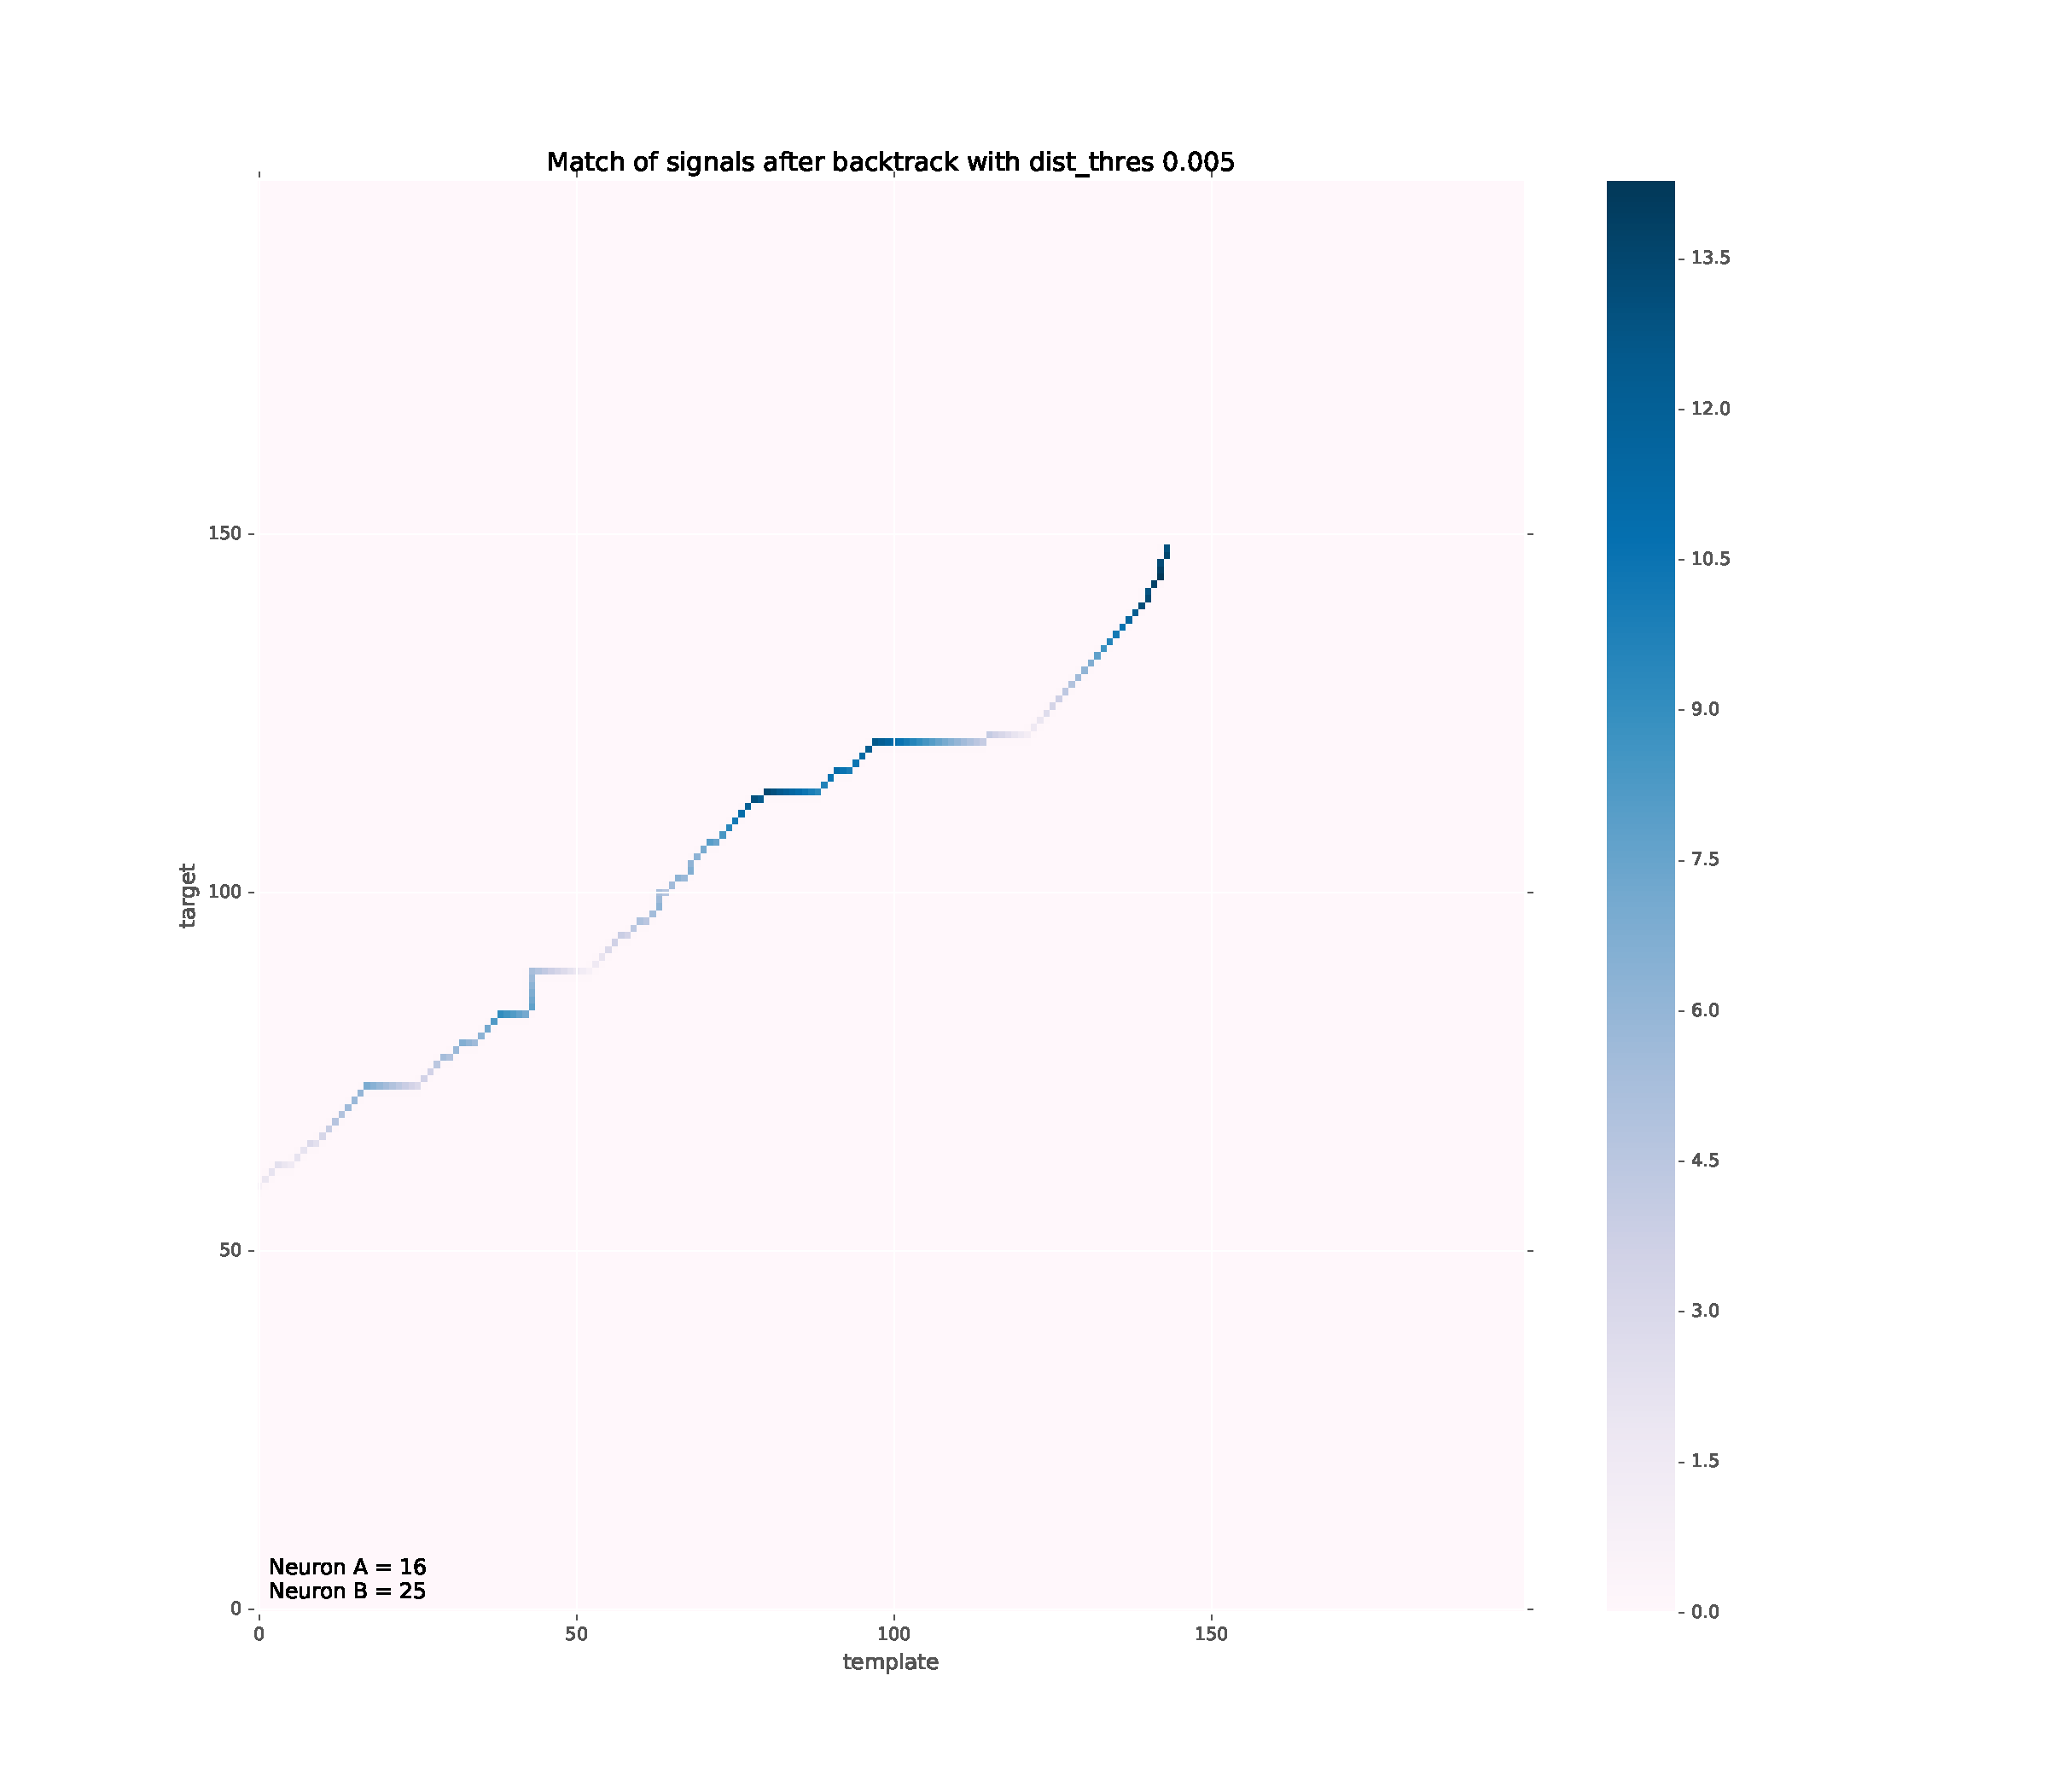
\includegraphics[width=\linewidth]{\plt/rlcsMain_backtrack_n1_16_n2_252016_05_06_11_00_24.pdf}
    \caption{RLCS score matrix}
    \label{fig:ori_simple}
  \end{subfigure}%
  \begin{subfigure}[b]{0.5\textwidth}
    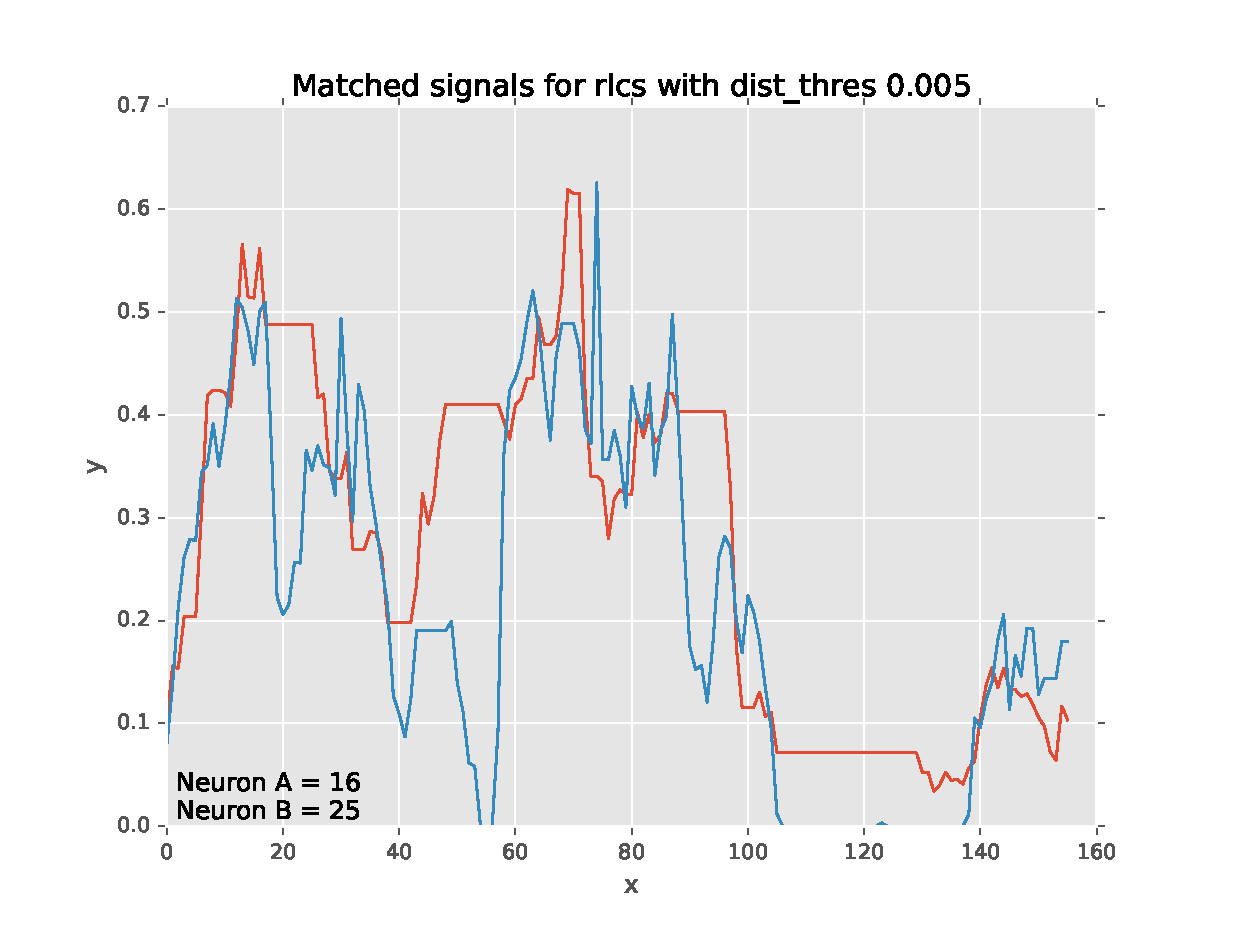
\includegraphics[width=\linewidth]{\plt/rlcsMain_getSegs_16_n2_252016_05_06_11_00_24}
    \caption{Extracted common subsequence}
    \label{fig:acfgram_diff}
  \end{subfigure}%
  \caption{Demonstration of RLCS score's dominance over Pearson correlation as a metric of similarity. RLCS analysis of two signals having low Pearson correlation. Extracted common subsequence was not detected by Pearson correlation.}
  \label{fig:oridir_simple}
\end{figure}
% subsection normalized_rlcs_score_as_a_correlation_metric (end)
% section rlcs (end)

%%%%%%%%%%%%%%%%%%%%%%%%%%%%%%%%%%%%%%%%%%%%%%%%%%%%%%%%%%%%%%%%%%%%%%
\chapter{Inferences and Future work}    % 3 pages
\label{chap:summary}
\section{Inferences} % (fold)
\label{sec:inferences}
Presence of motifs in neuronal responses is confirmed and it provided motivation to study motifs using RLCS algorithm. In the intertrial responses of a neuron, simple correlation measure failed to detect reliability of response. By extracting motifs from the same, we were able to obtain reliable subsequences of significant length ($\sim 60 - 120$ samples out from total of 200 samples) across trials. The similarity in signals could be attributed to reliability of information representation and similar activation mechanism of neurons. 

As an effort to study response similarities of two neurons in a mice, common subsequence spotting is performed on time-series responses of two different neurons. The study resulted in detection of motifs of significant length ($\sim 40 - 60$ samples out from total of 200 samples) across neurons. Even after the receptive fields of two neurons being different, The presence of motifs could be due to information encoding by correlation of a population, neuronal interconnection and similar activation mechanism of neurons.

Responses of neurons across different mice are analyzed for the presence of motifs. The study is not expected to give long motifs as the two neurons are independent. The experimental results showed presence of common subsequences but as expected, the subsequences are small in length ($\sim 15 - 30$ samples out from total of 200 samples). This could be attributed to similar activation mechanism of neurons. Exceptionally, few neurons across different mice produced longer subsequences (of length $\sim 50$ samples). Inferring meaning of this exception is left as future work.
% section inferences (end)
\section{Future work} % (fold)
\label{sec:future_work}
The presence of significant motifs in neuronal signals is established in this work. But the impact the result has in the context of Neuroscience is yet to be studied. We have not studied the significance of signal extracted as a motif. We formulated a better measure for correlation between neurons. Interneuronal correlations play a great role in information encoding in brain. With the new correlation measure, information coding with inter-neuronal correlations can be studied further.

The current RLCS algorithm penalize a constant value for any mismatch. It does not take care how much the samples mismatch. The penalization can be selected as a function of distance between samples. This will create a better match of signals. 
% section future_work (end)


%%%%%%%%%%%%%%%%%%%%%%%%%%%%%%%%%%%%%%%%%%%%%%%%%%%%%%%%%%%%%%%%%%%%%%
\appendix
\chapter{Additional results from RLCS}
\label{chap:rlcsplots_appndx}
Chapter ~\ref{sec:rlcs} presented only few examples of motif extraction for brevity. Additional results are provided here for reference. Each result consist of RLCS score matrix and longest motif extracted. Results are categorized based on neurons considered for the study.
\section{RLCS of intertrial responses} % (fold)
\label{sec:rlcs_between_intertrial_responses}
\begin{figure}[h]
  \begin{subfigure}[b]{0.5\textwidth}
    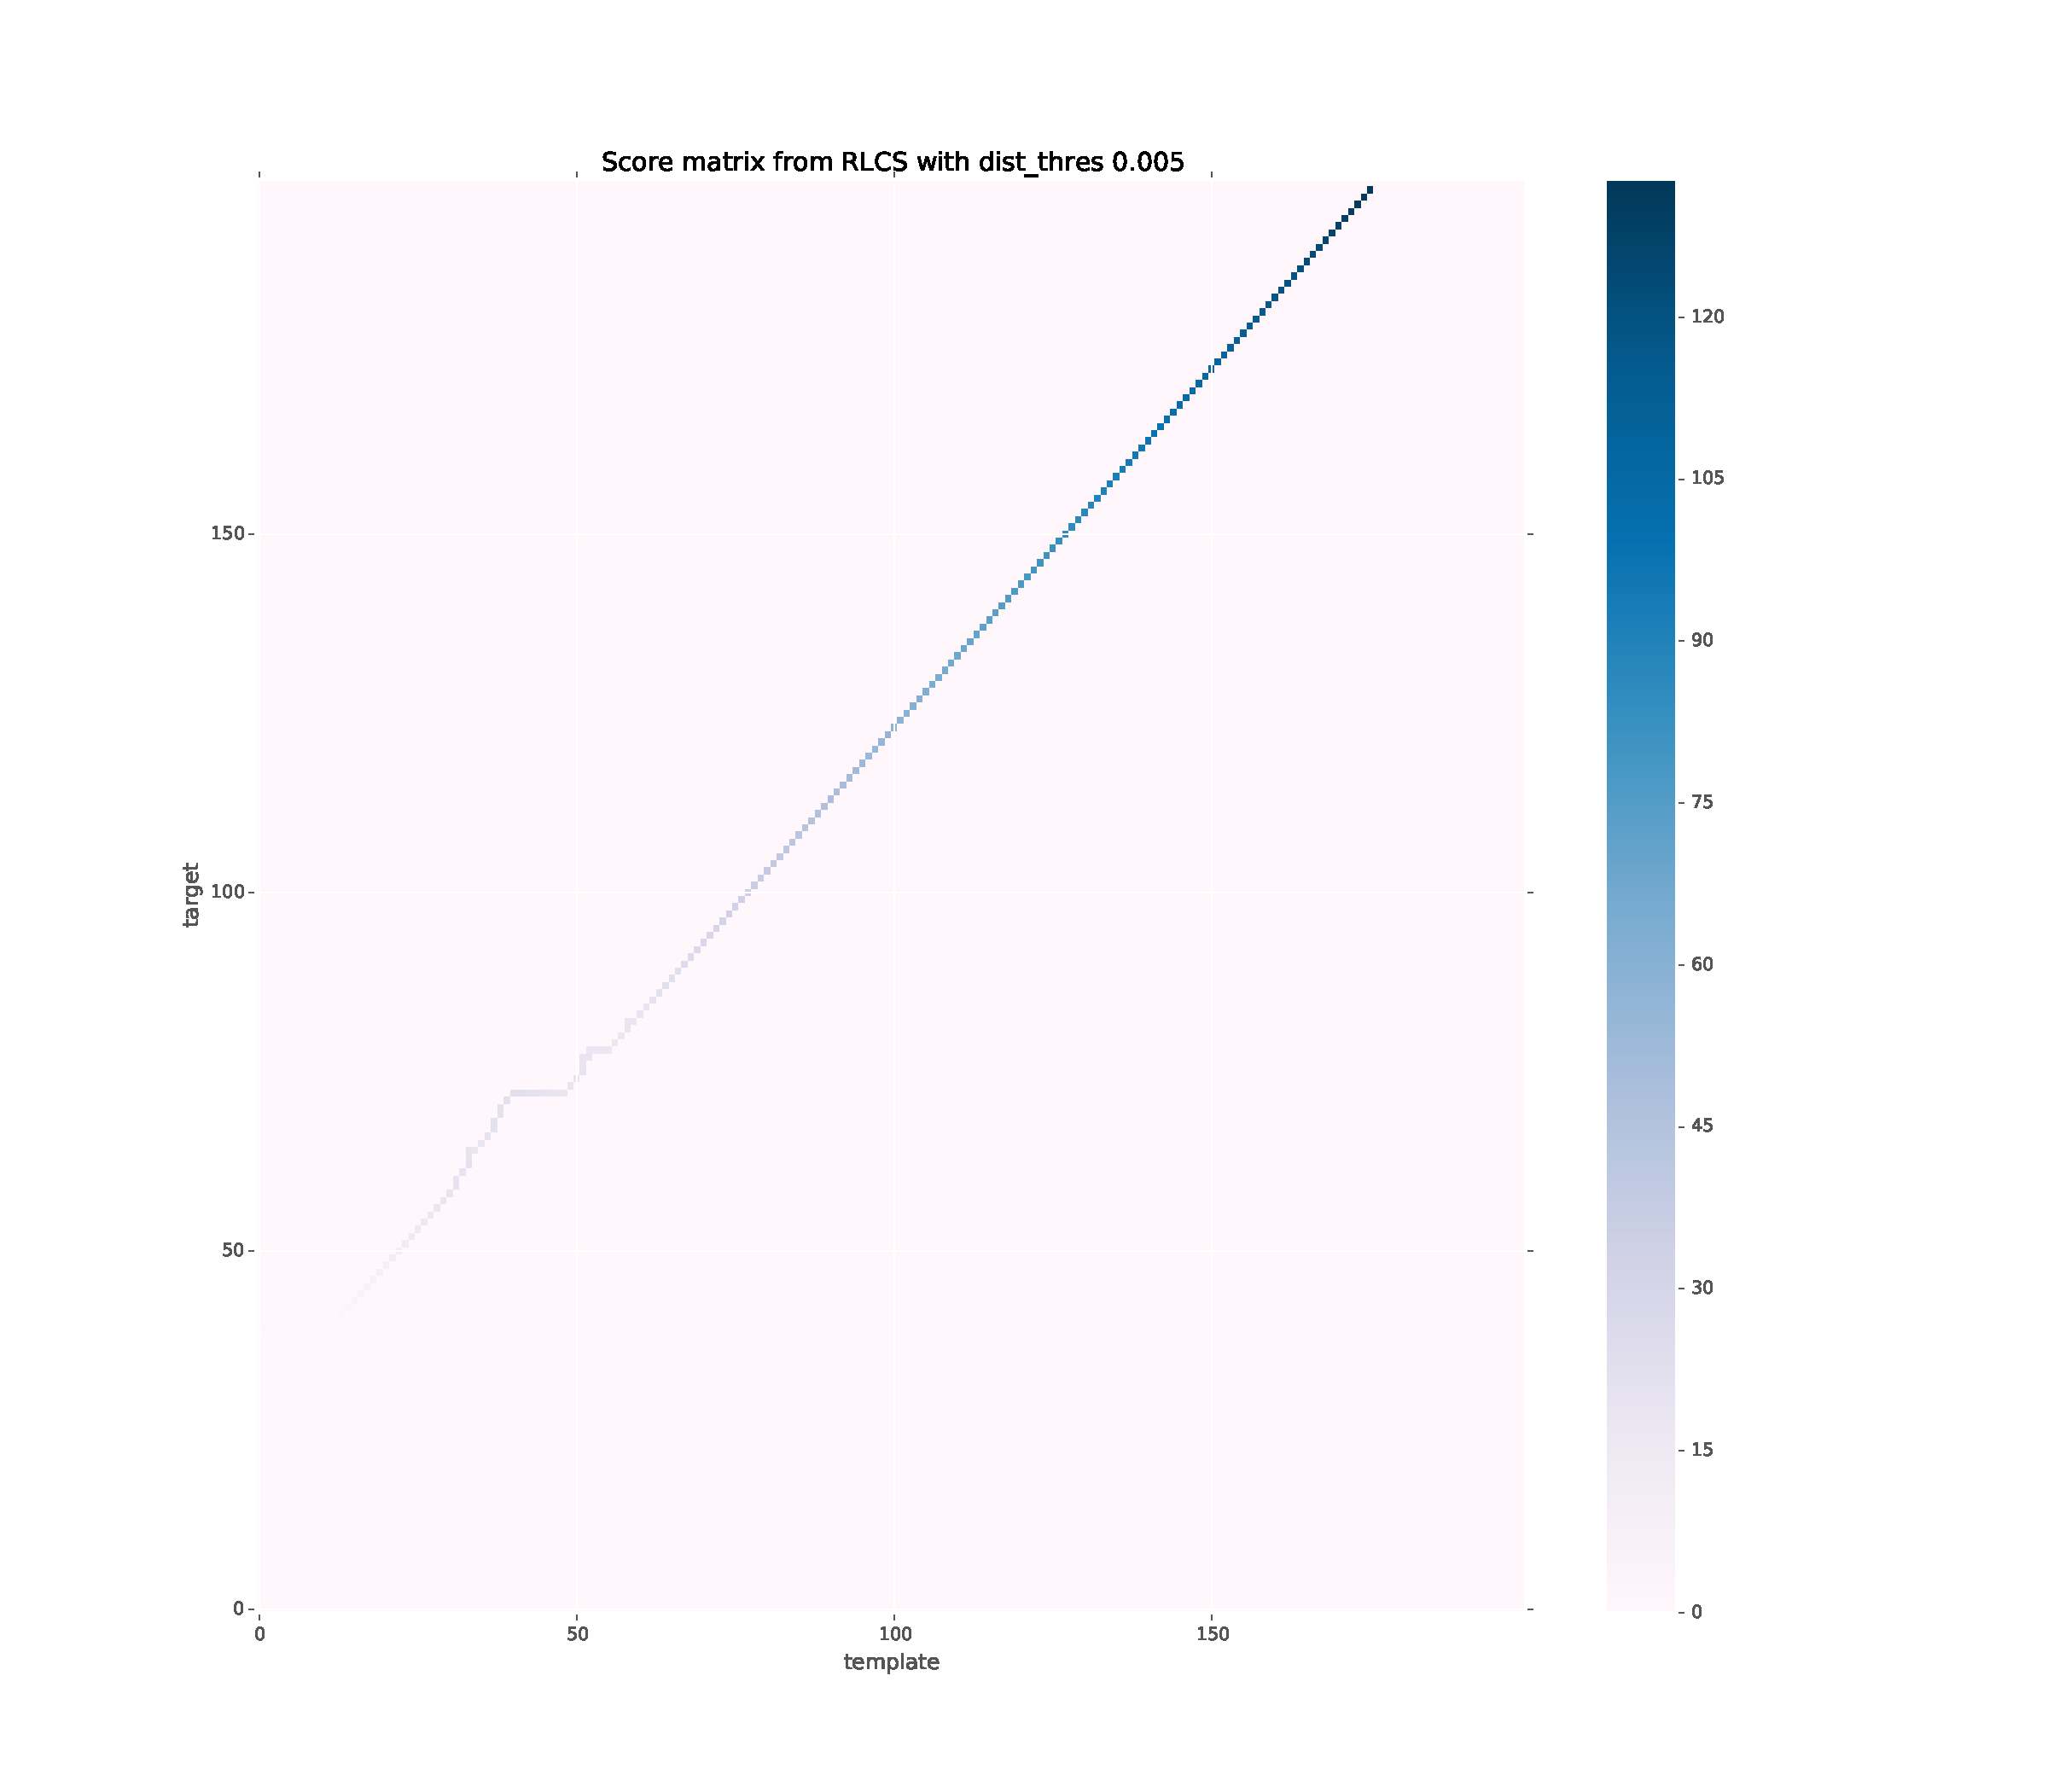
\includegraphics[width=\linewidth]{\plt/apndx/rlcsMain_score_trial_0_1n_222016_05_08_19_04_26.pdf}
    \caption{Score matrix}
  \end{subfigure}%
  \begin{subfigure}[b]{0.5\textwidth}
    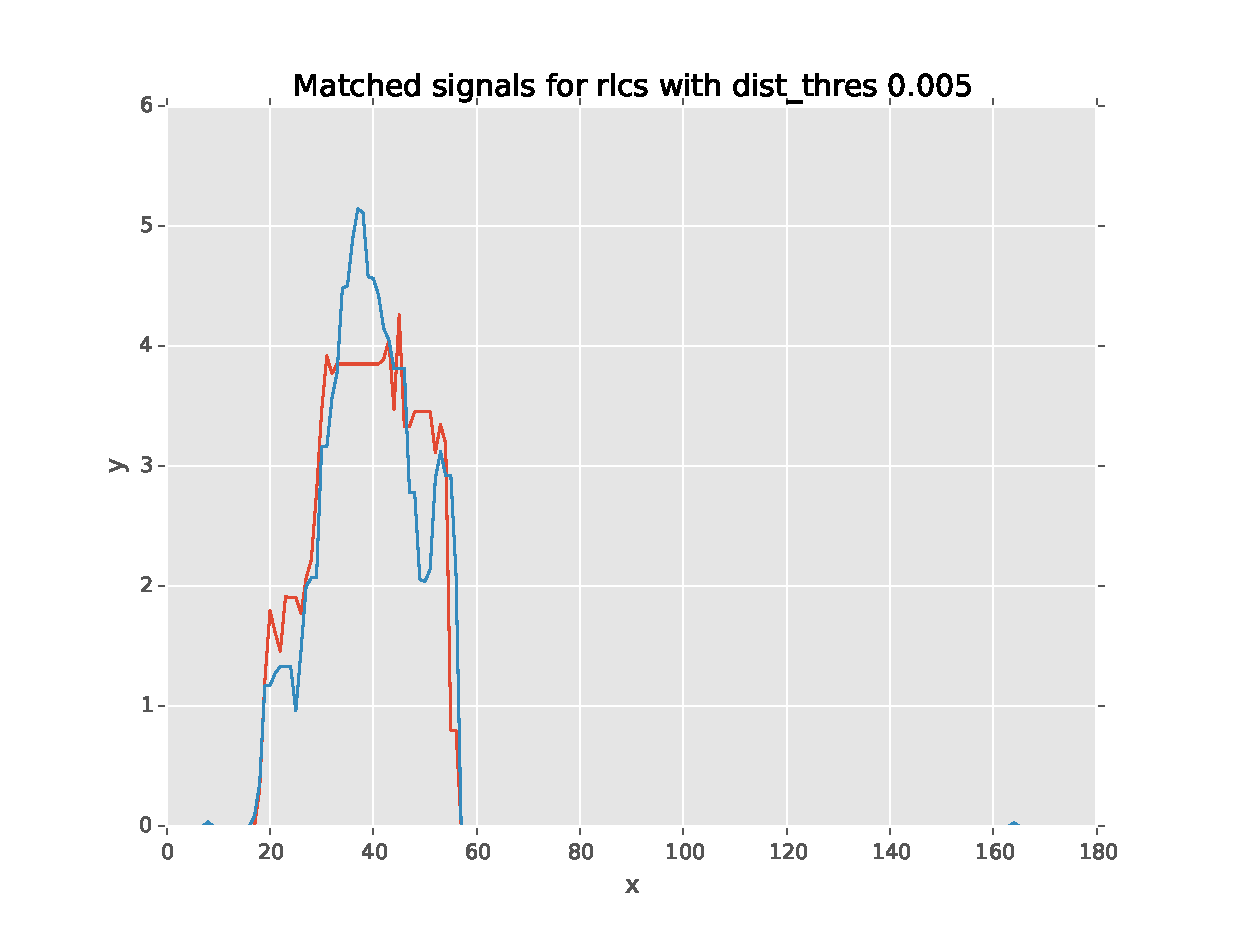
\includegraphics[width=\linewidth]{\plt/apndx/rlcsMain_motif_trial_0_1n_222016_05_08_19_04_26}
    \caption{Extracted longest motif}
  \end{subfigure}%
  \caption{RLCS performed on intertrial responses of a neuron. Note the presence of $\sim 150$ sample subsequence which is undetectable in Pearson correlation test.}
  \label{fig:}
\end{figure}

\begin{figure}[h]
  \begin{subfigure}[b]{0.5\textwidth}
    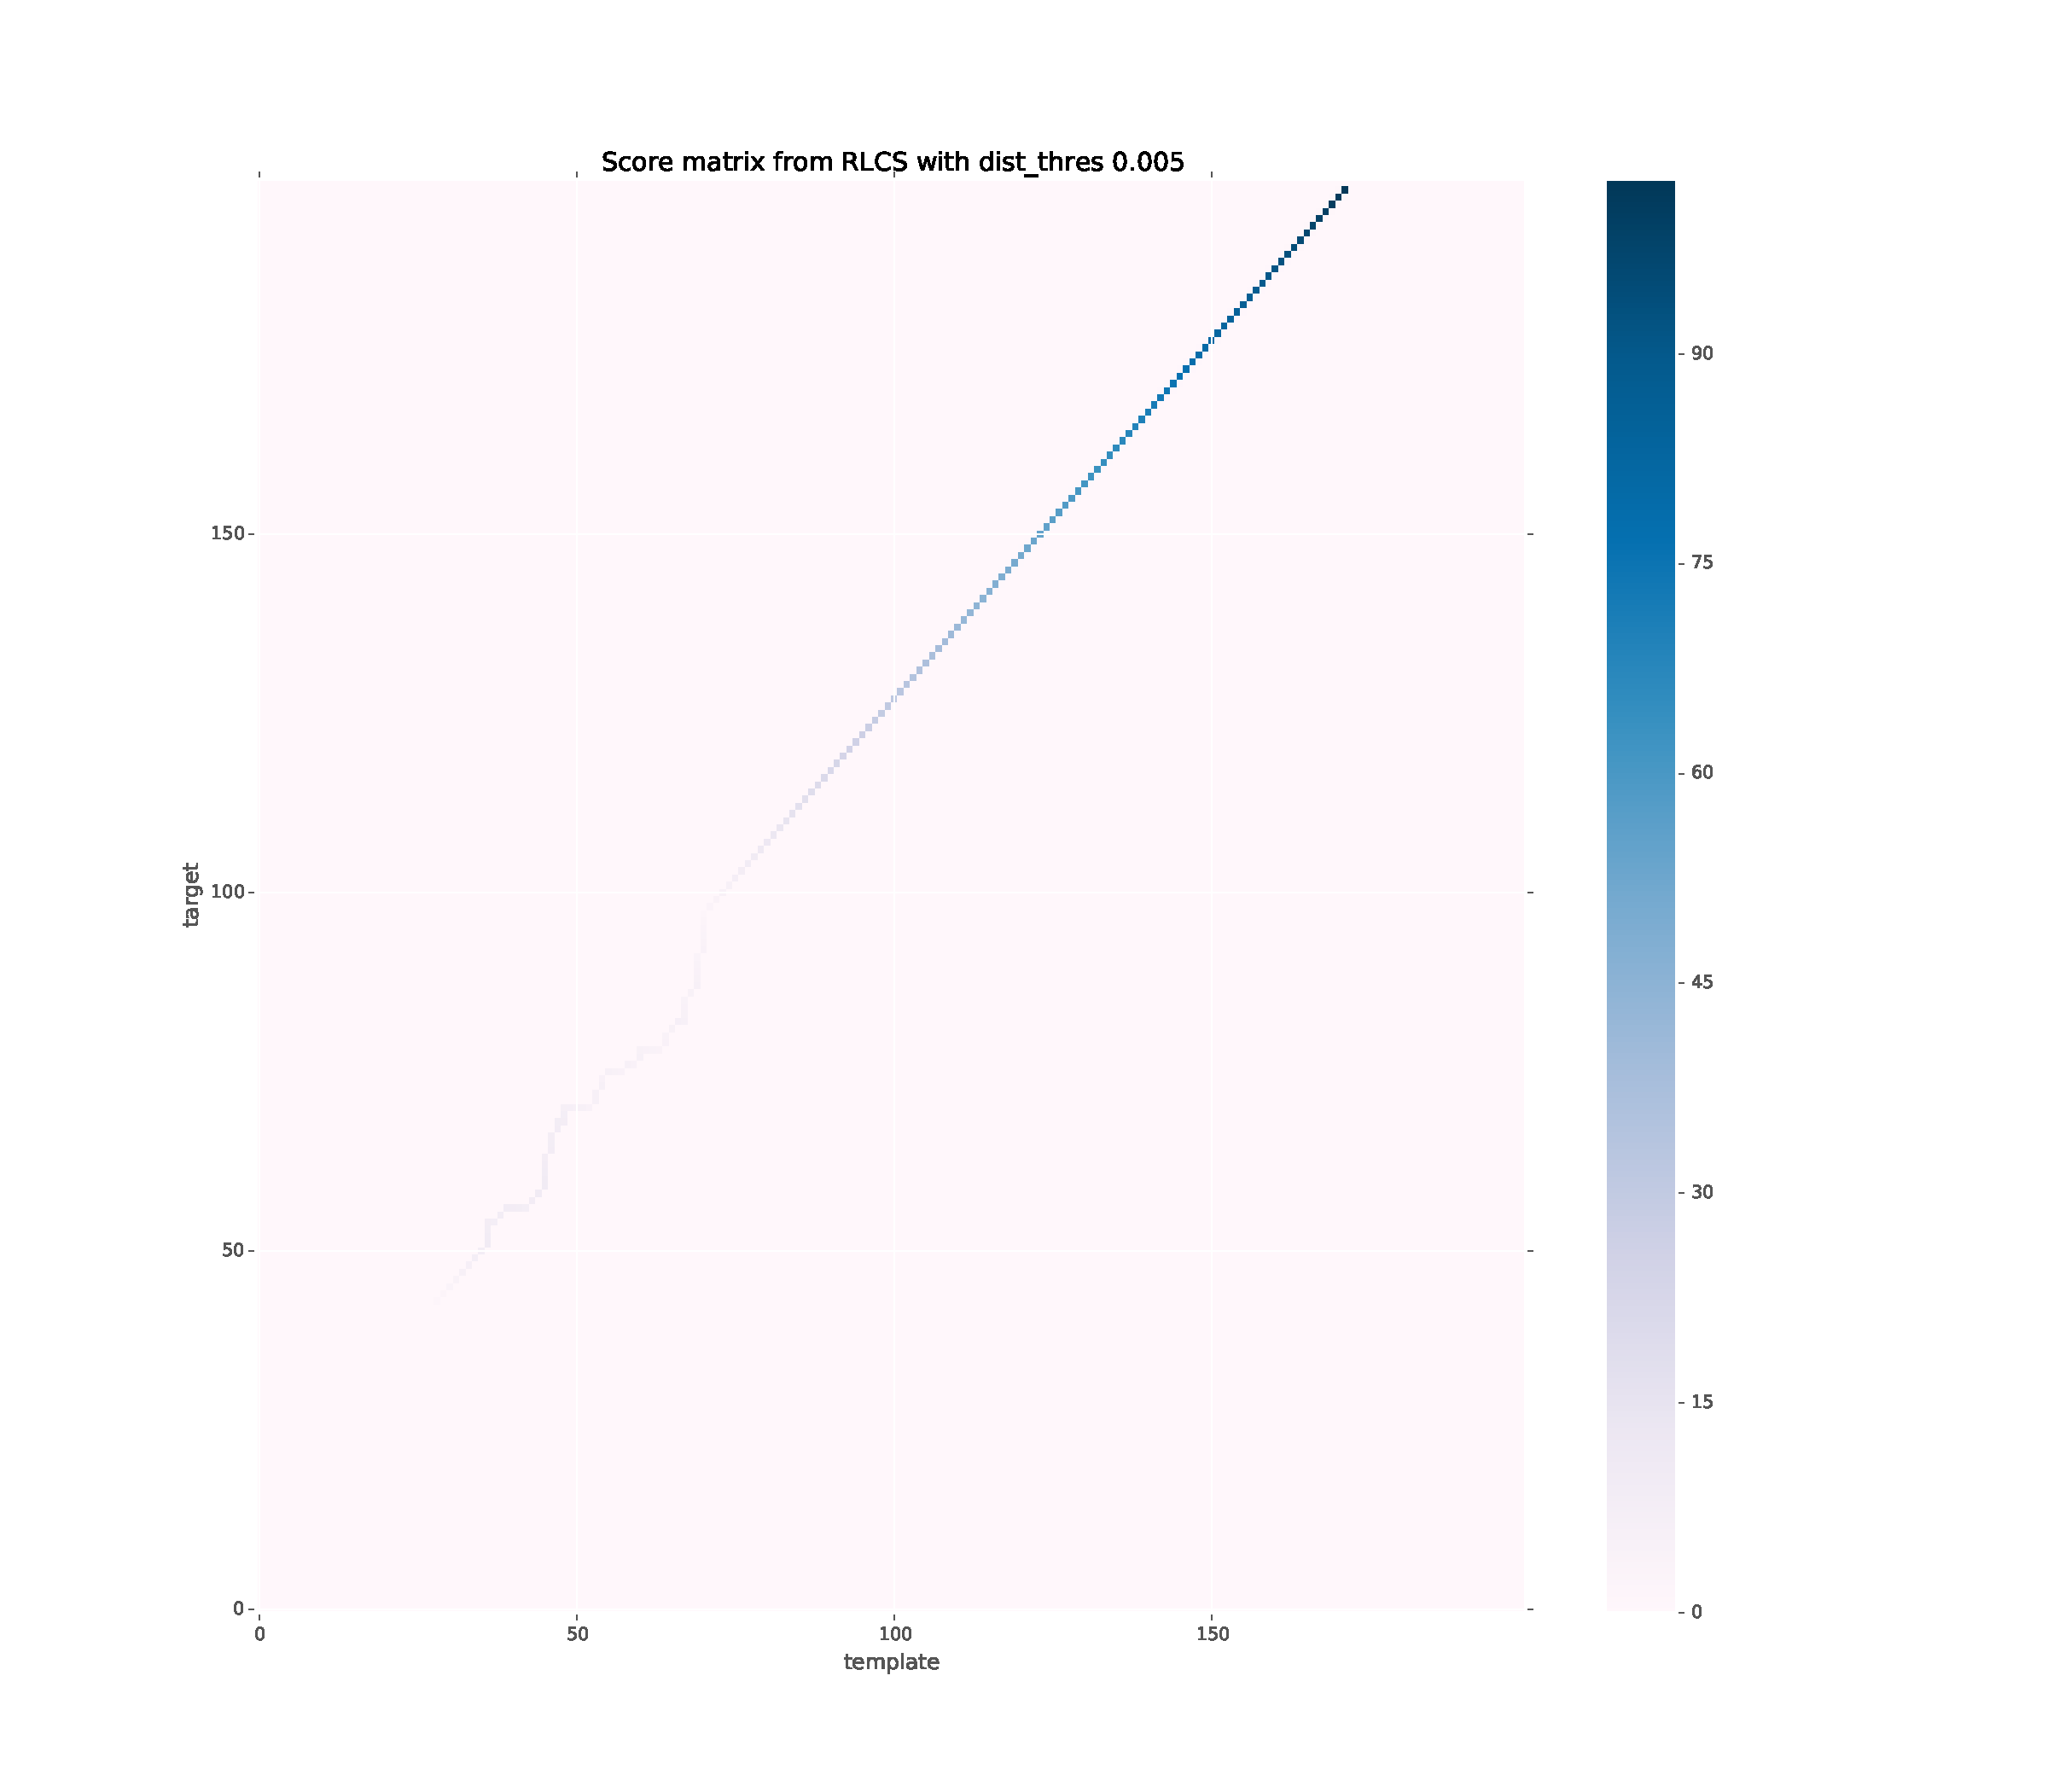
\includegraphics[width=\linewidth]{\plt/apndx/rlcsMain_score_trial_0_1n_322016_05_08_19_14_28.pdf}
    \caption{Score matrix}
  \end{subfigure}%
  \begin{subfigure}[b]{0.5\textwidth}
    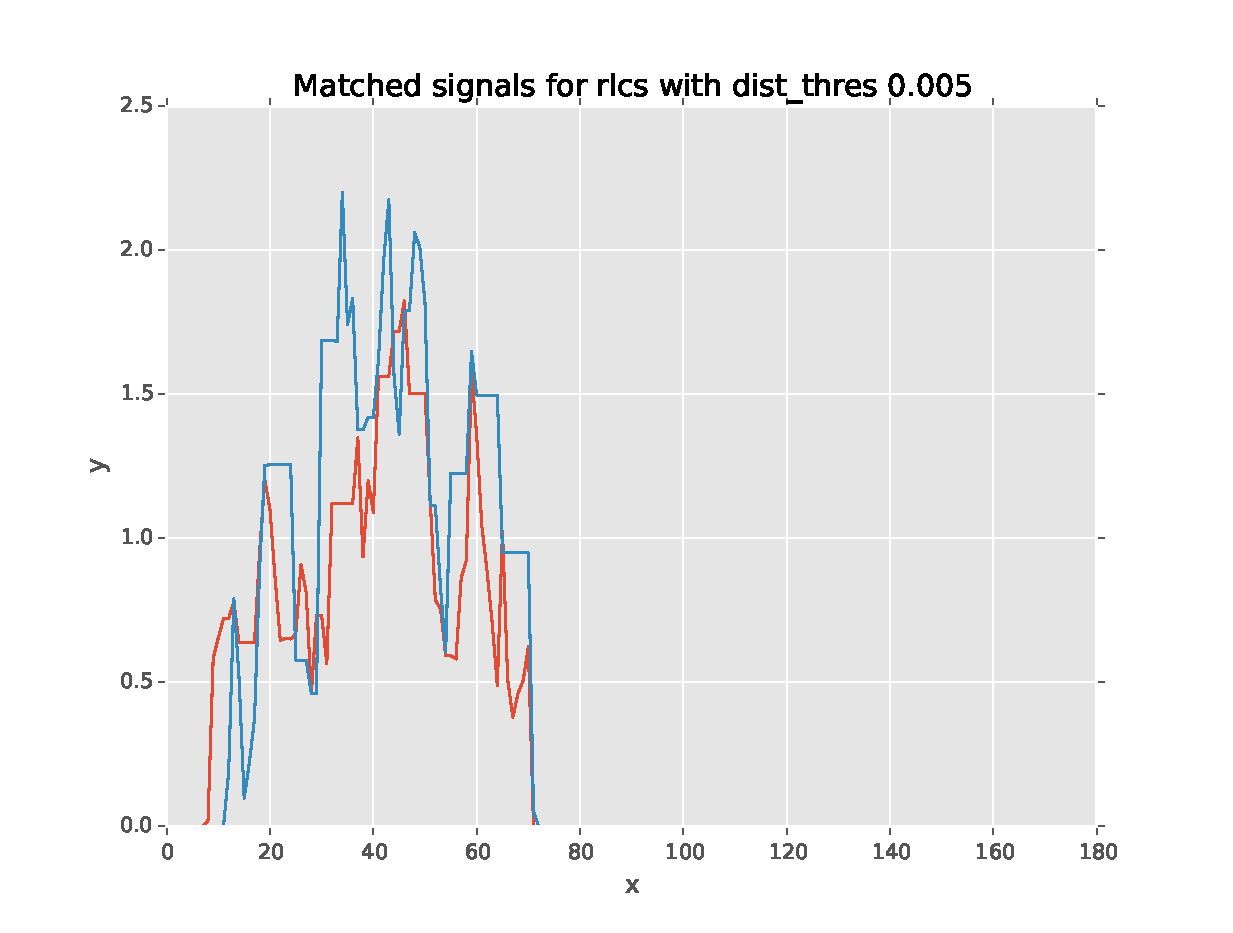
\includegraphics[width=\linewidth]{\plt/apndx/rlcsMain_motif_trial_0_1n_322016_05_08_19_14_28}
    \caption{Extracted longest motif}
  \end{subfigure}%
  \caption{RLCS performed on intertrial responses of a neuron. Note the presence of $\sim 150$ sample subsequence which is undetectable in Pearson correlation test.}
  \label{fig:}
\end{figure}

\begin{figure}[h]
  \begin{subfigure}[b]{0.5\textwidth}
    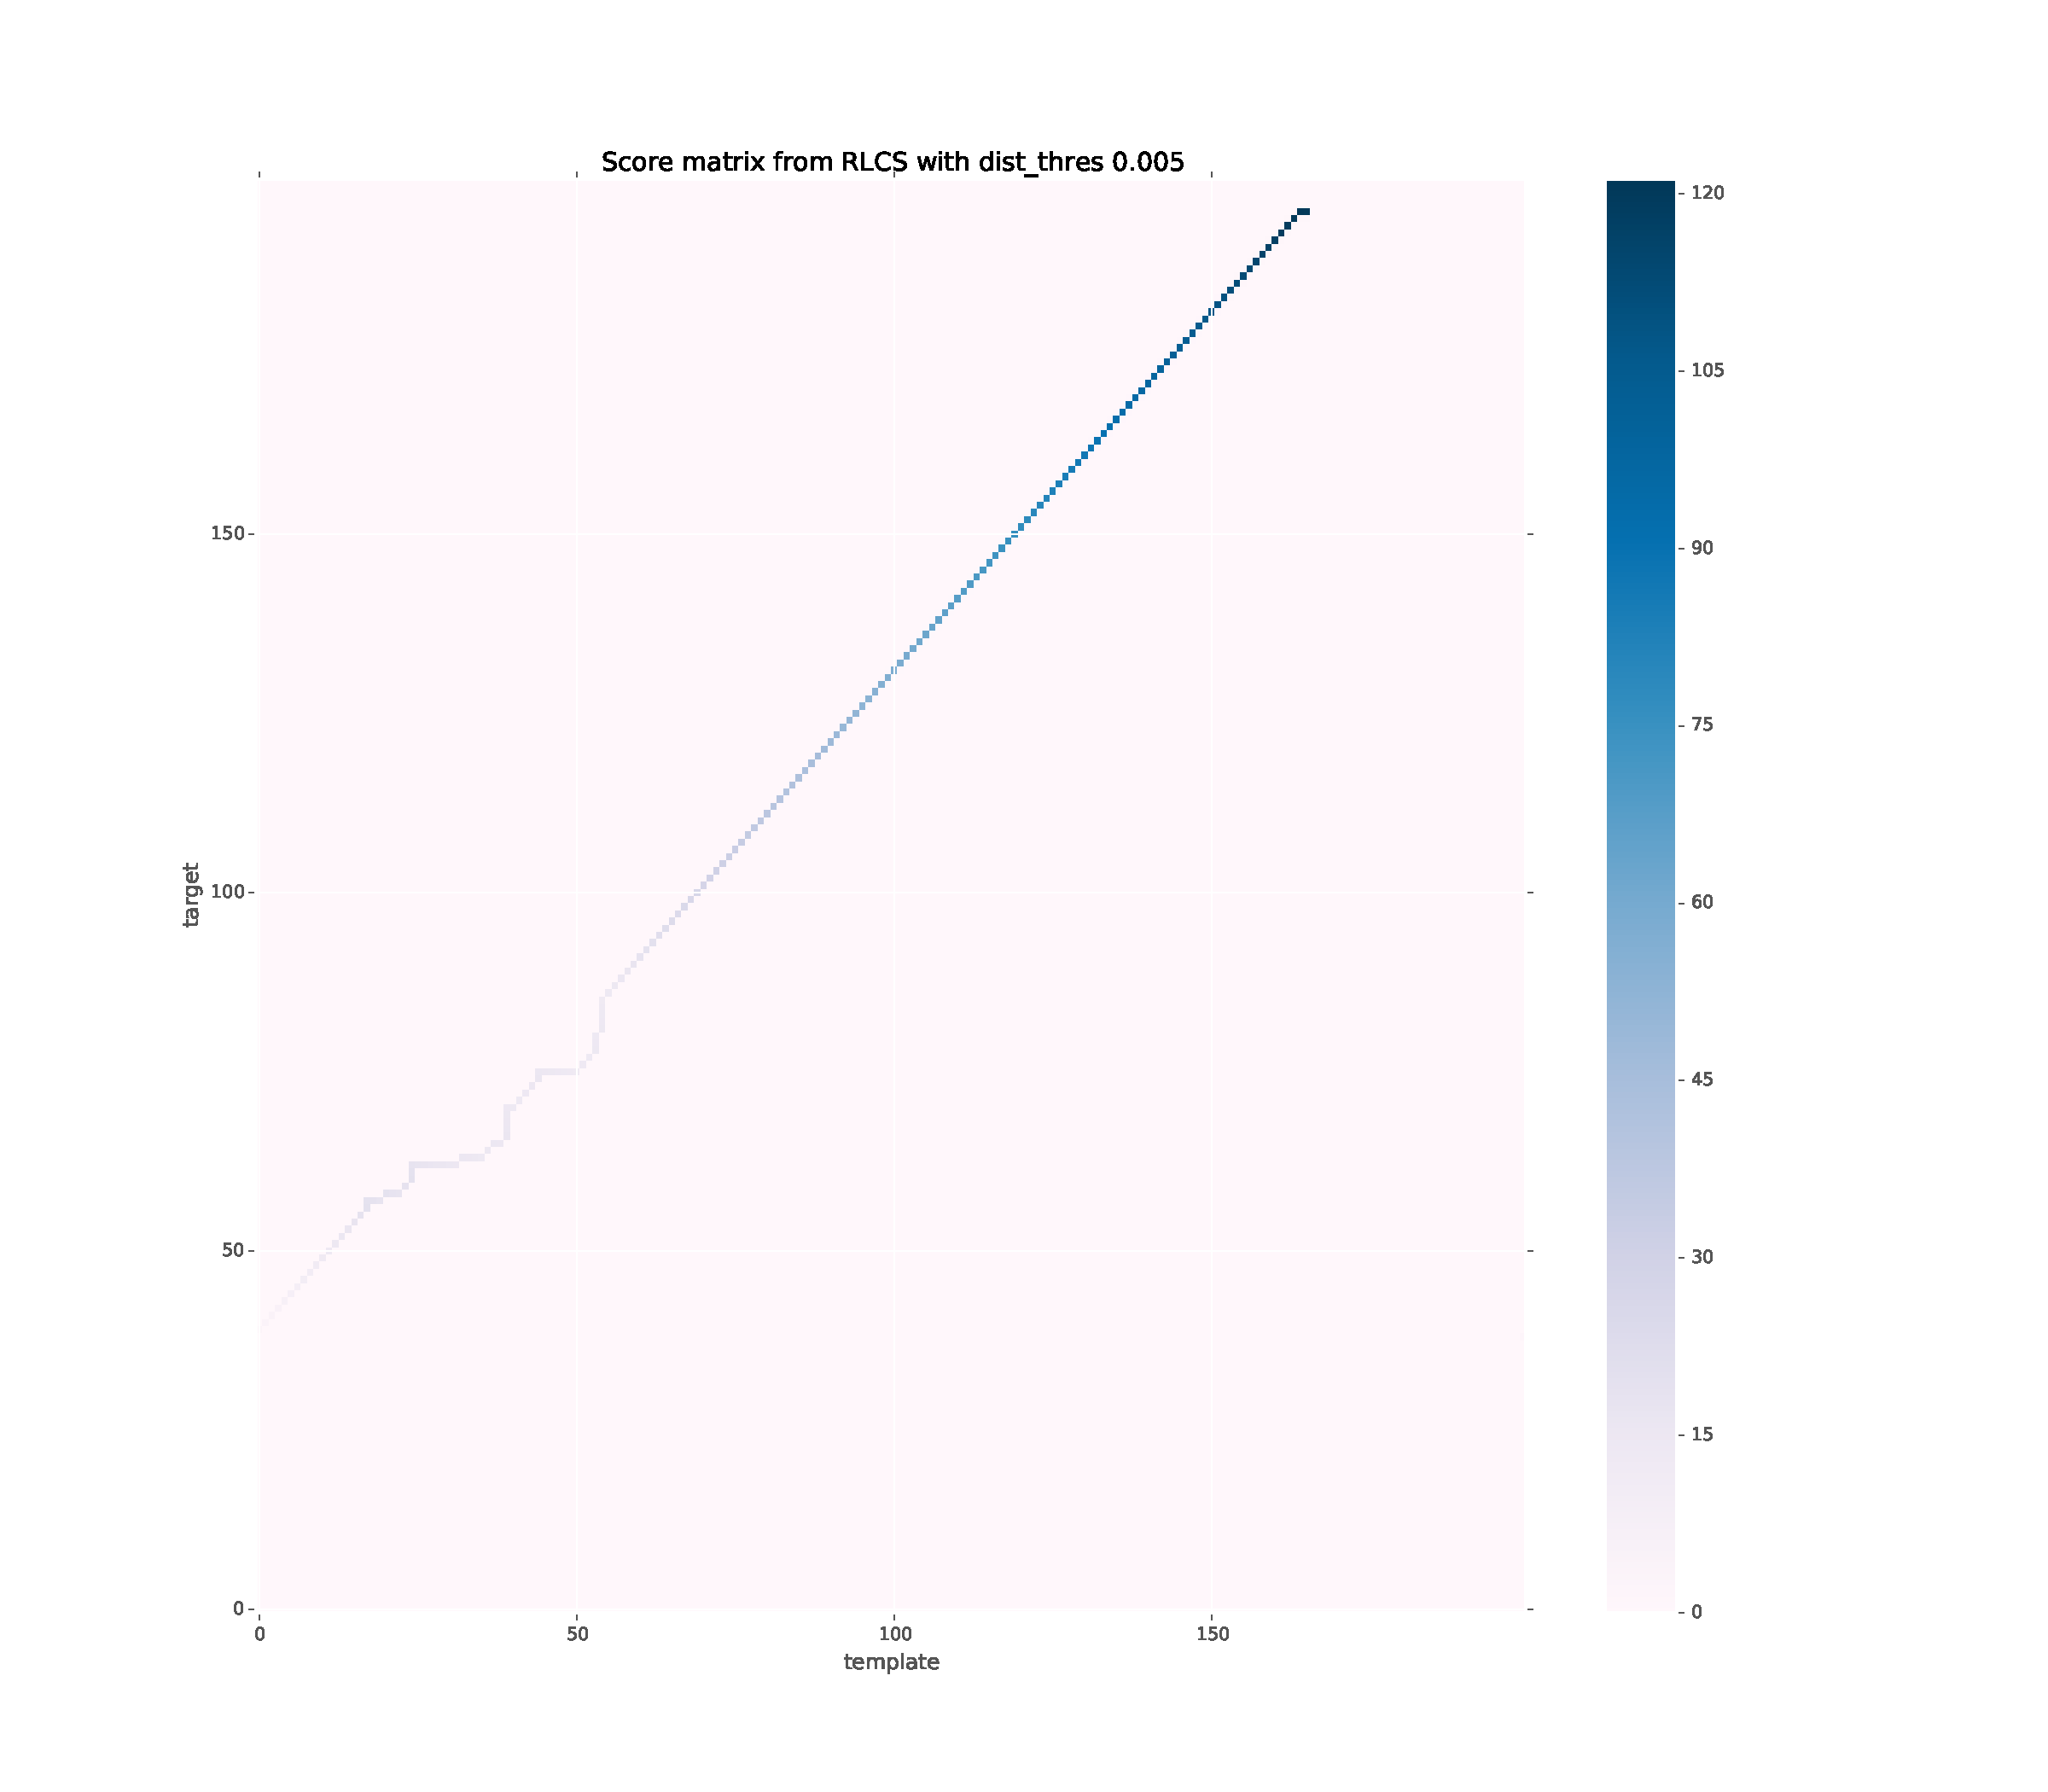
\includegraphics[width=\linewidth]{\plt/apndx/rlcsMain_score_trial_0_1n_422016_05_08_19_18_34.pdf}
    \caption{Score matrix}
  \end{subfigure}%
  \begin{subfigure}[b]{0.5\textwidth}
    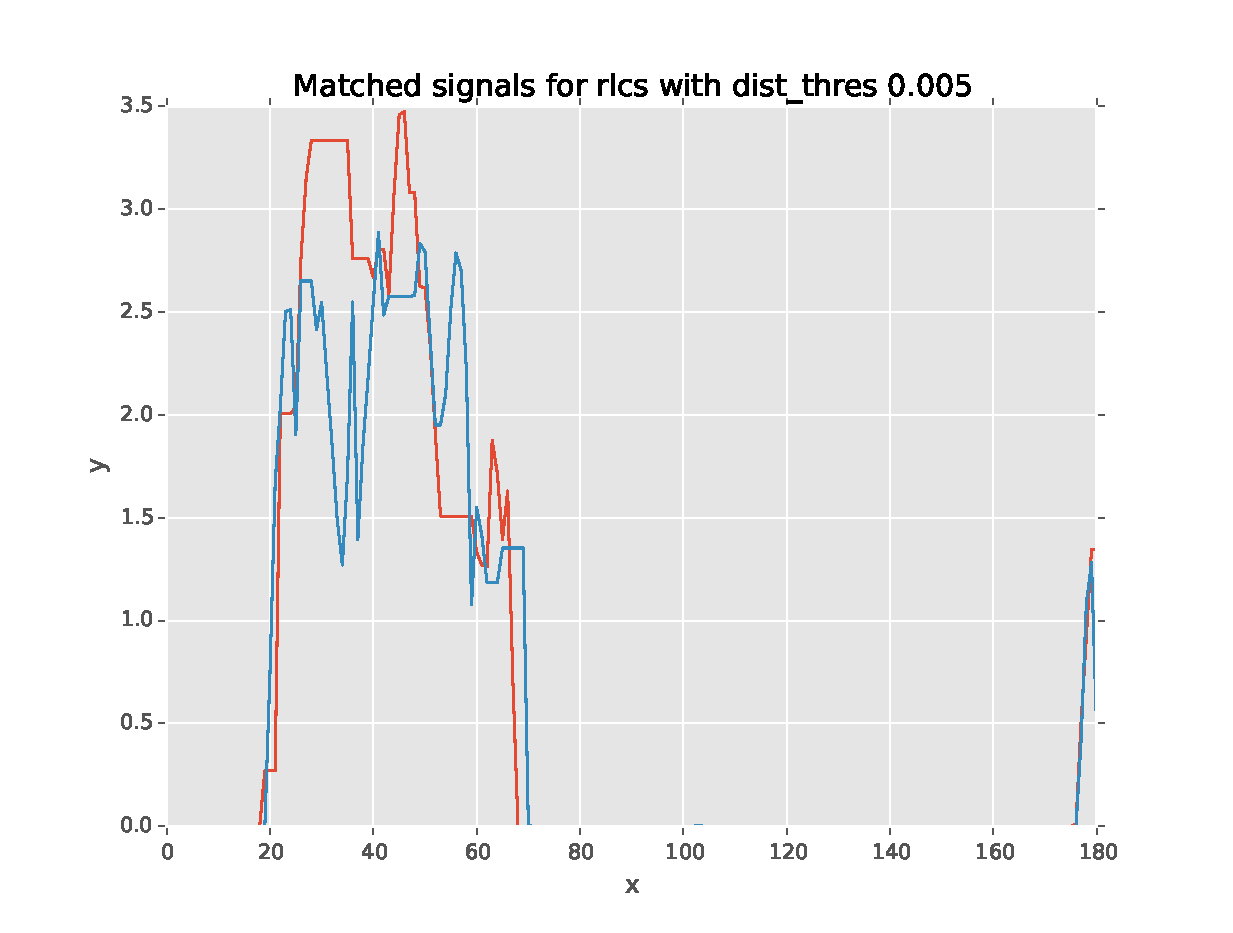
\includegraphics[width=\linewidth]{\plt/apndx/rlcsMain_motif_trial_0_1n_422016_05_08_19_18_33}
    \caption{Extracted longest motif}
  \end{subfigure}%
  \caption{RLCS performed on intertrial responses of a neuron. Note the presence of $\sim 150$ sample subsequence which is undetectable in Pearson correlation test.}
  \label{fig:}
\end{figure}

% section rlcs_between_intertrial_responses (end)
\FloatBarrier
\section{RLCS of responses from two neurons in a mouse} % (fold)
\label{sec:rlcs_of_responses_from_two_neurons_in_a_mouse}
\begin{figure}[h]
  \begin{subfigure}[b]{0.5\textwidth}
    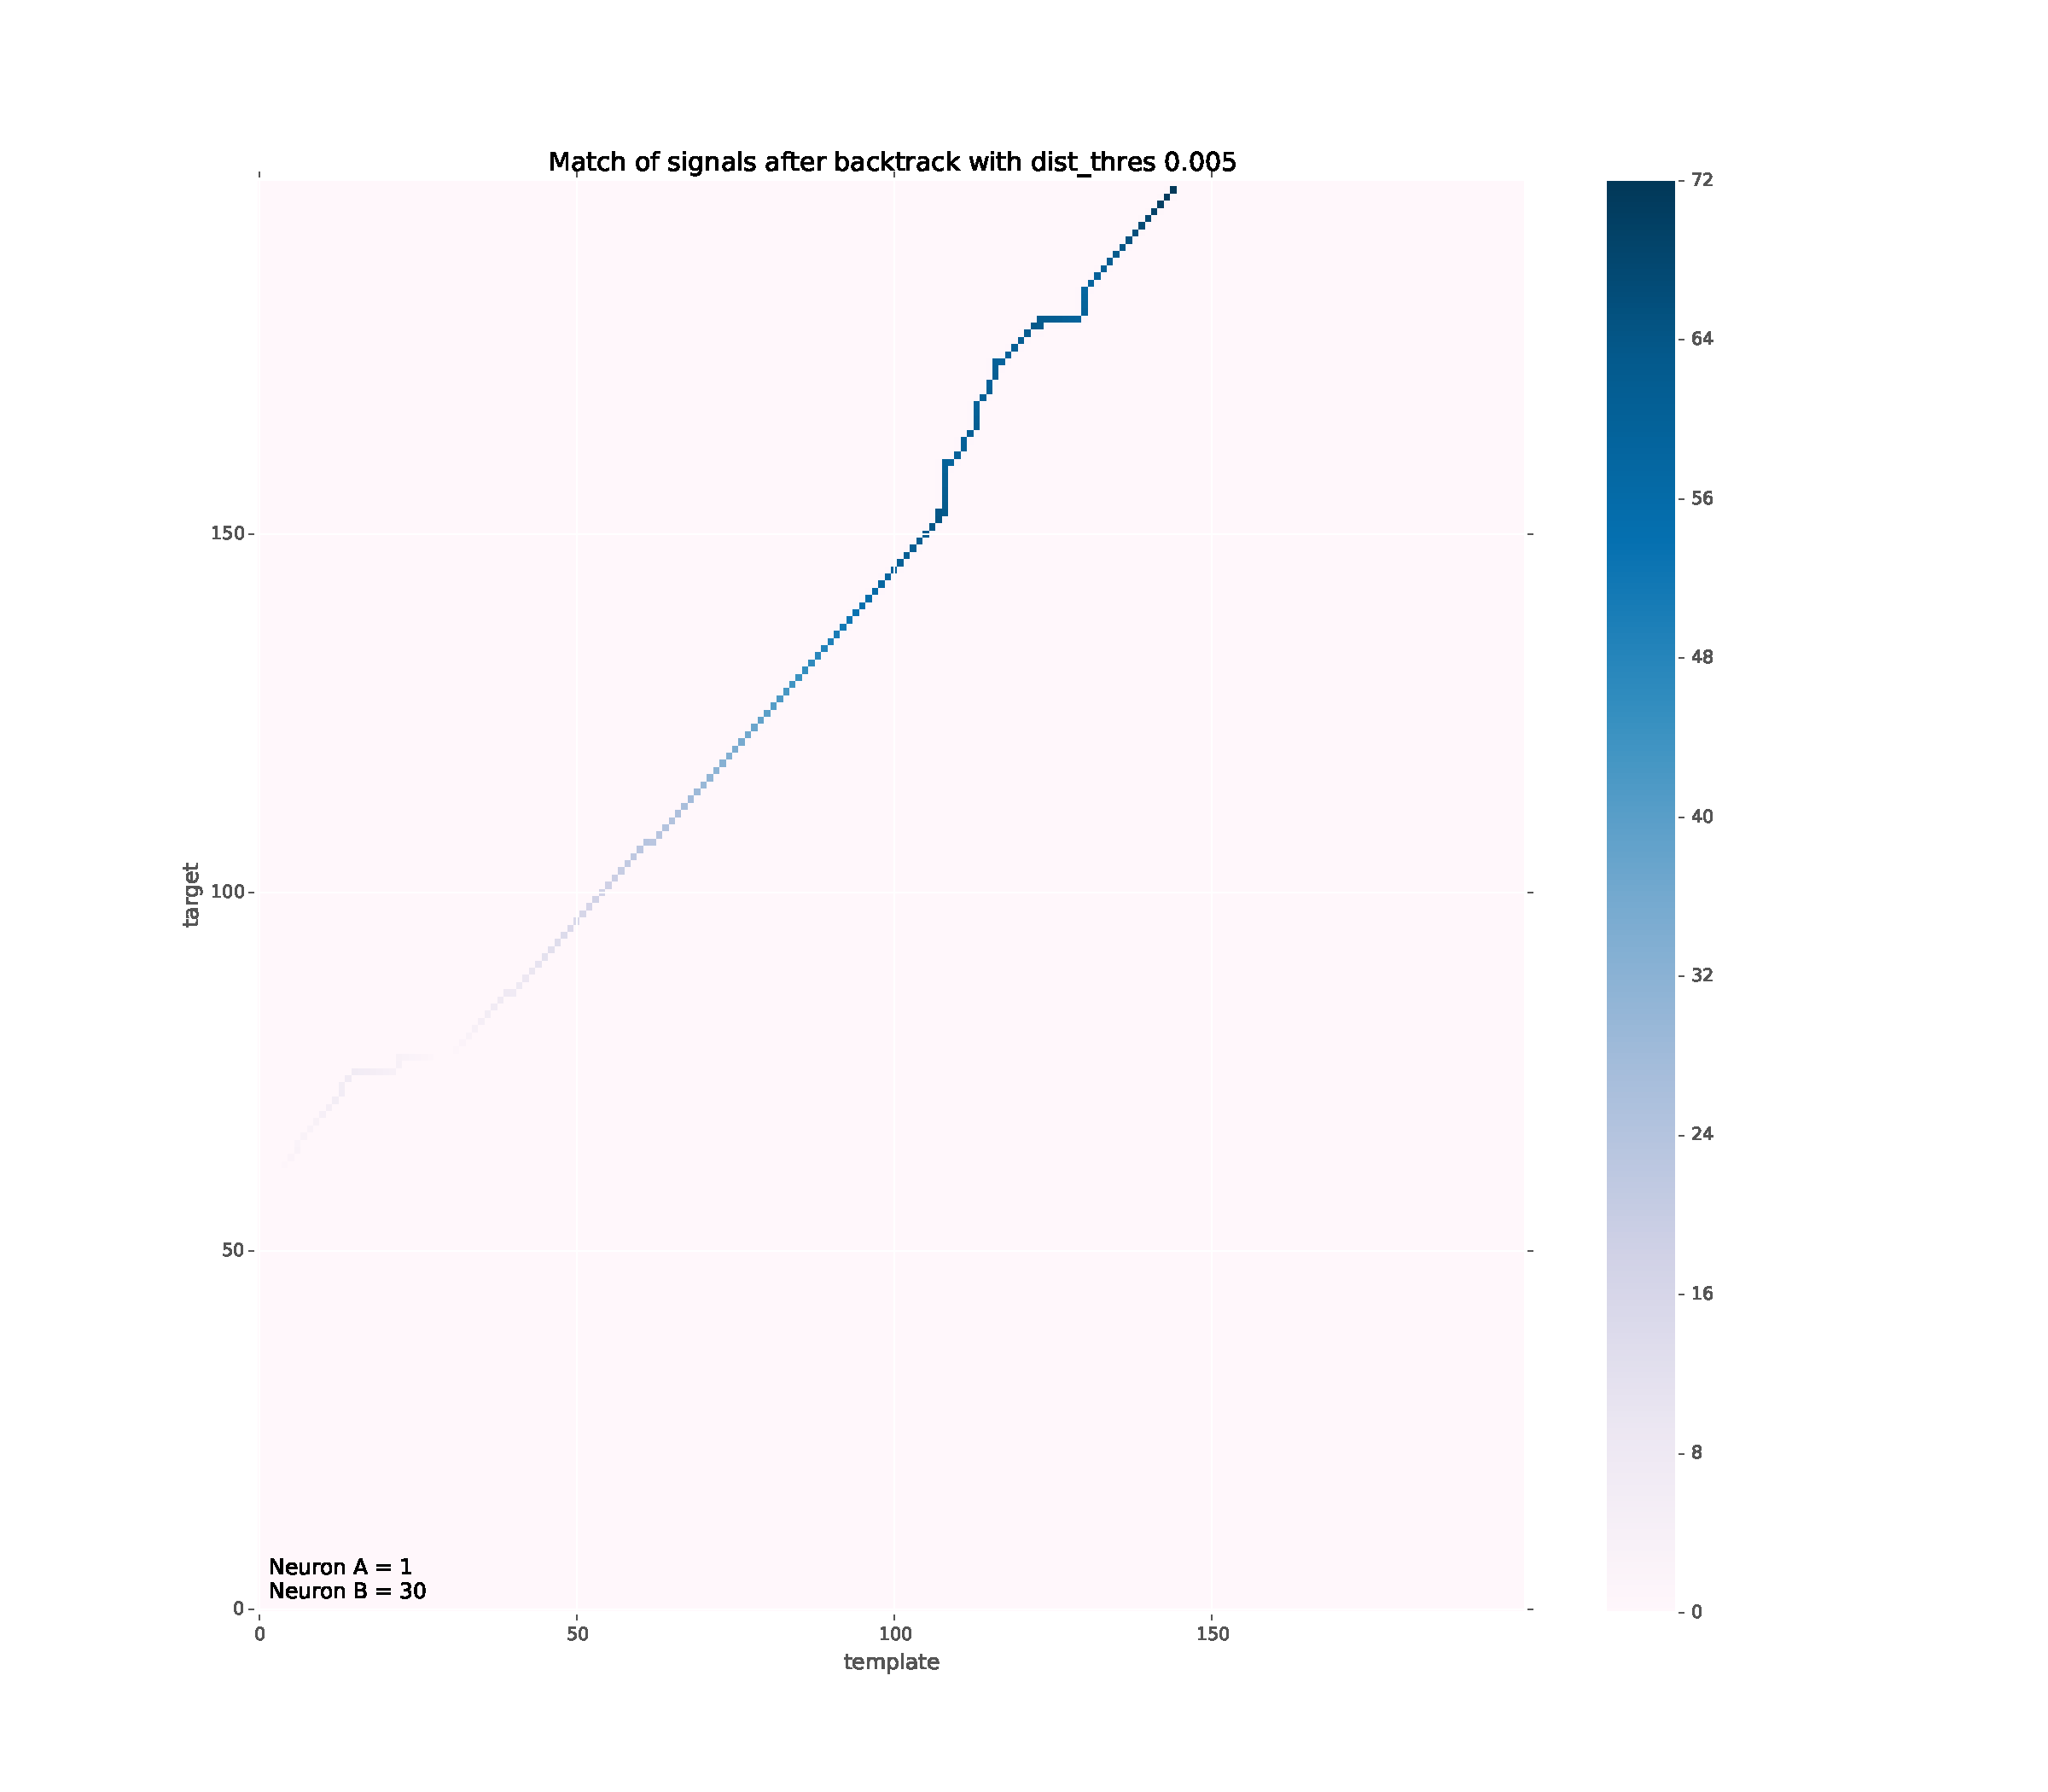
\includegraphics[width=\linewidth]{\plt/apndx/rlcsMain_backtrack_n1_1_n2_302016_05_08_19_22_31.pdf}
    \caption{Score matrix}
  \end{subfigure}%
  \begin{subfigure}[b]{0.5\textwidth}
    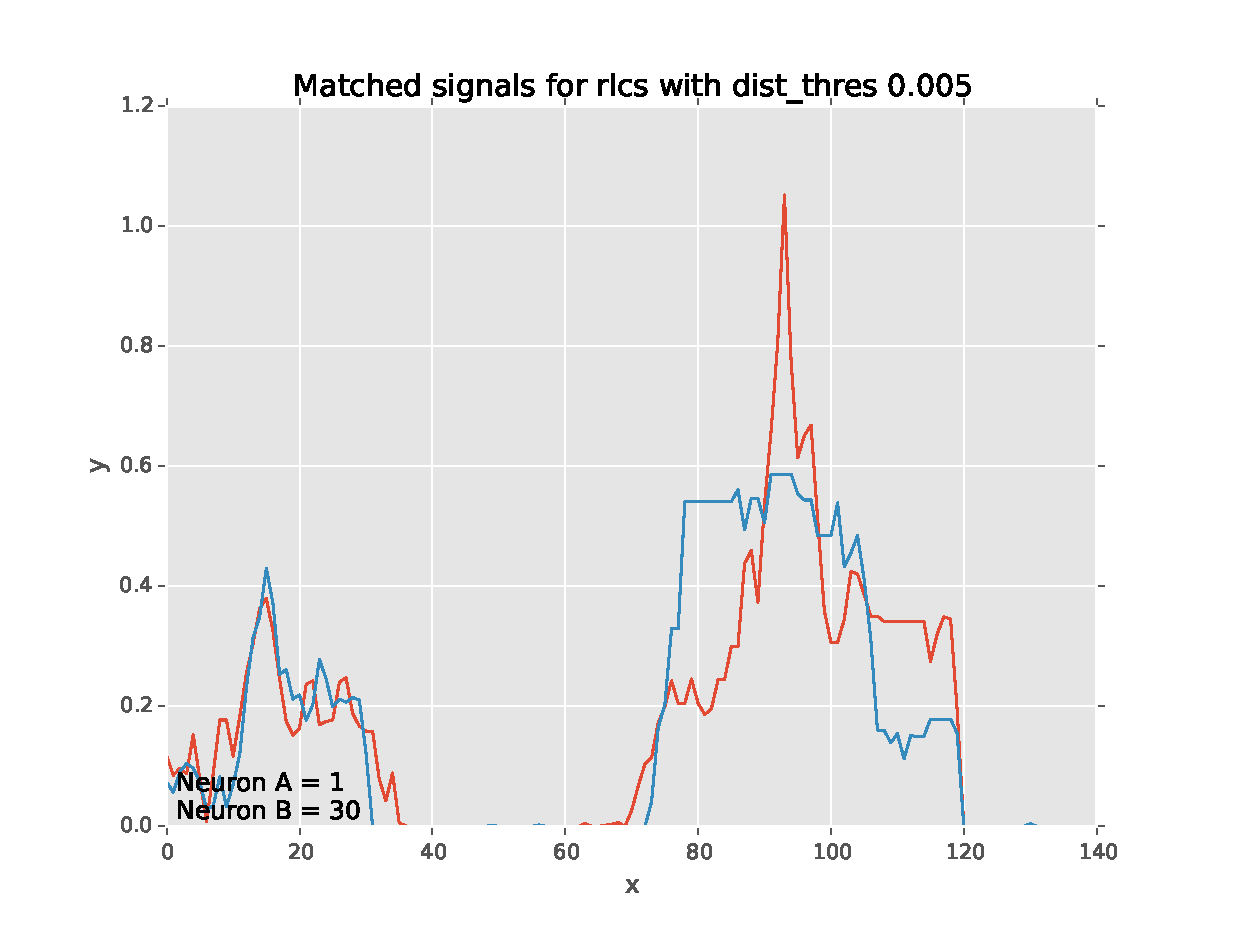
\includegraphics[width=\linewidth]{\plt/apndx/rlcsMain_getSegs_1_n2_302016_05_08_19_22_31}
    \caption{Extracted longest motif}
  \end{subfigure}%
  \caption{RLCS performed on responses of two neurons within a mouse. The two signals have a pearson correlation of 0.18}
  \label{fig:}
\end{figure}

\begin{figure}[h]
  \begin{subfigure}[b]{0.5\textwidth}
    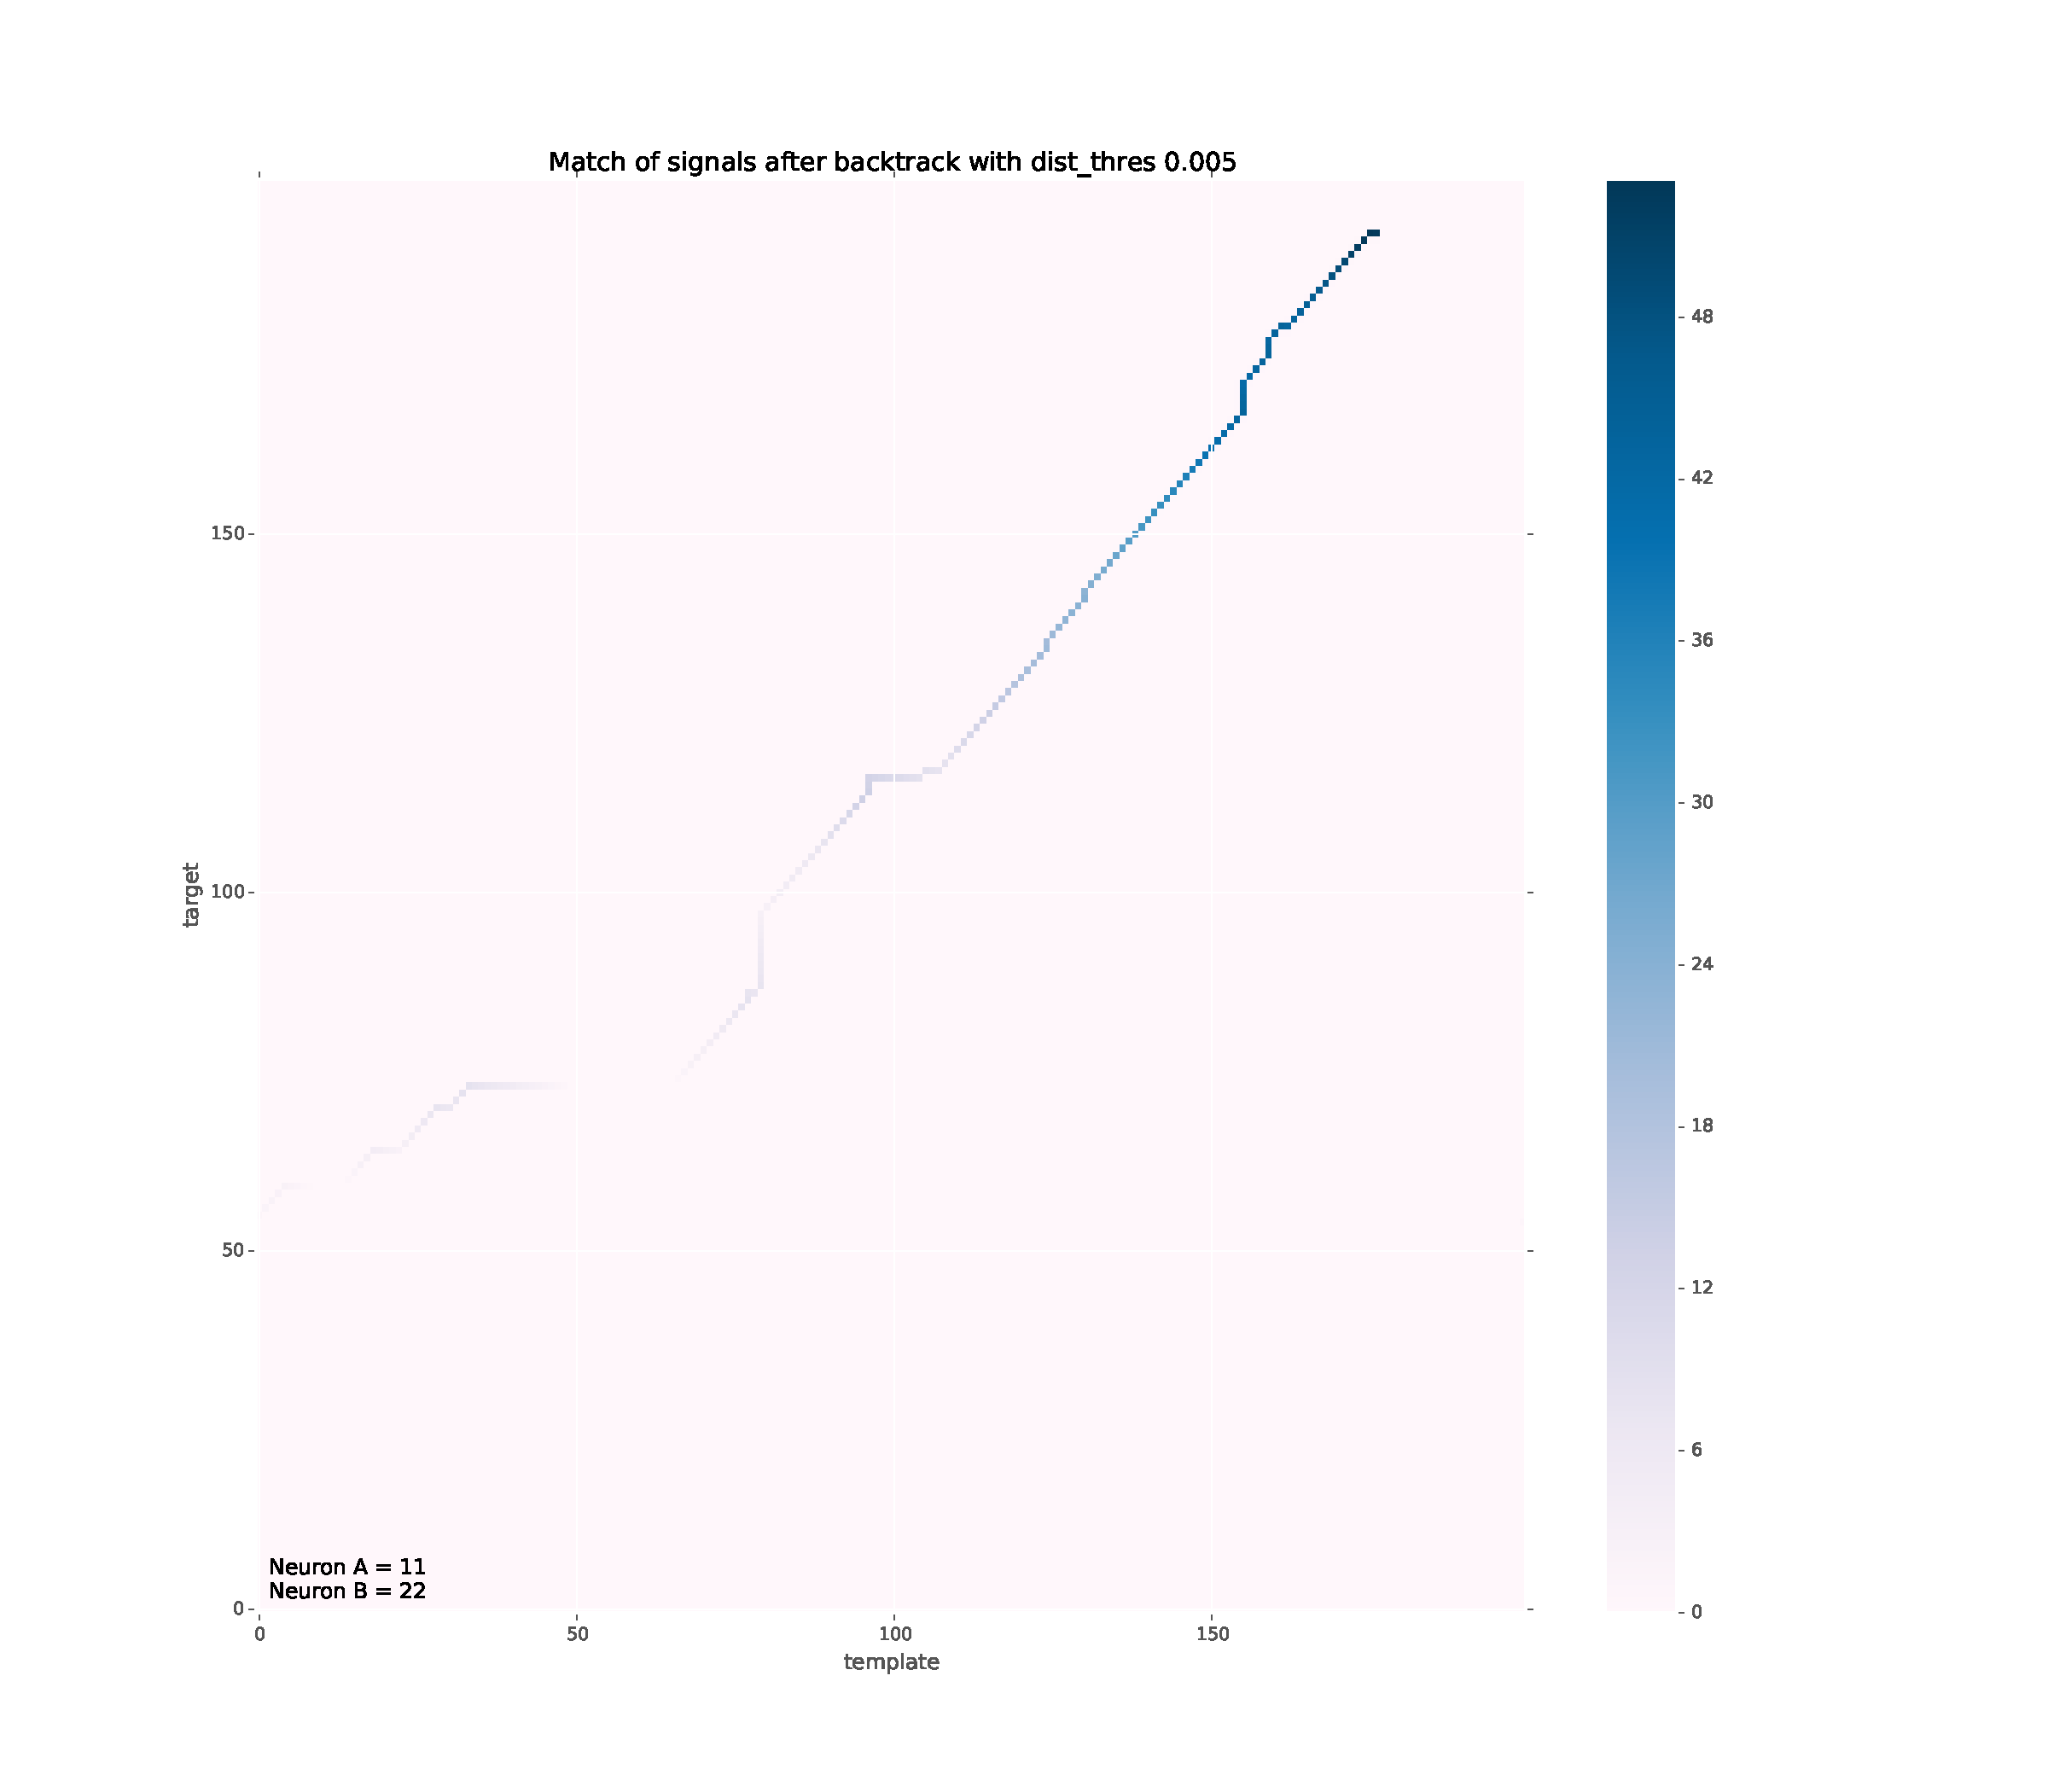
\includegraphics[width=\linewidth]{\plt/apndx/rlcsMain_backtrack_n1_11_n2_222016_05_08_19_25_22.pdf}
    \caption{Score matrix}
  \end{subfigure}%
  \begin{subfigure}[b]{0.5\textwidth}
    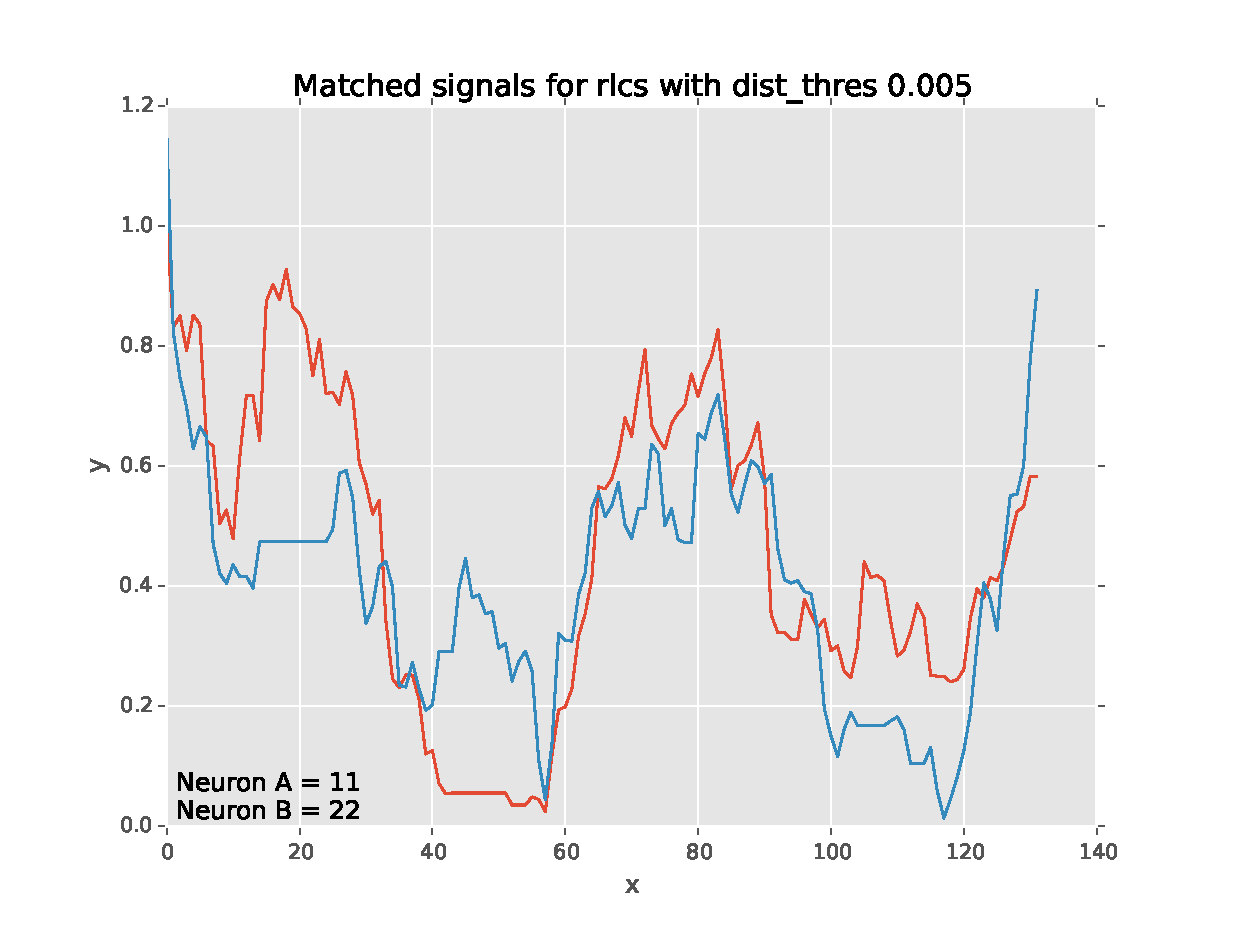
\includegraphics[width=\linewidth]{\plt/apndx/rlcsMain_getSegs_11_n2_222016_05_08_19_25_22}
    \caption{Extracted longest motif}
  \end{subfigure}%
  \caption{RLCS performed on responses of two neurons within a mouse. The two signals have a pearson correlation of 0.06}
  \label{fig:}
\end{figure}

\begin{figure}[h]
  \begin{subfigure}[b]{0.5\textwidth}
    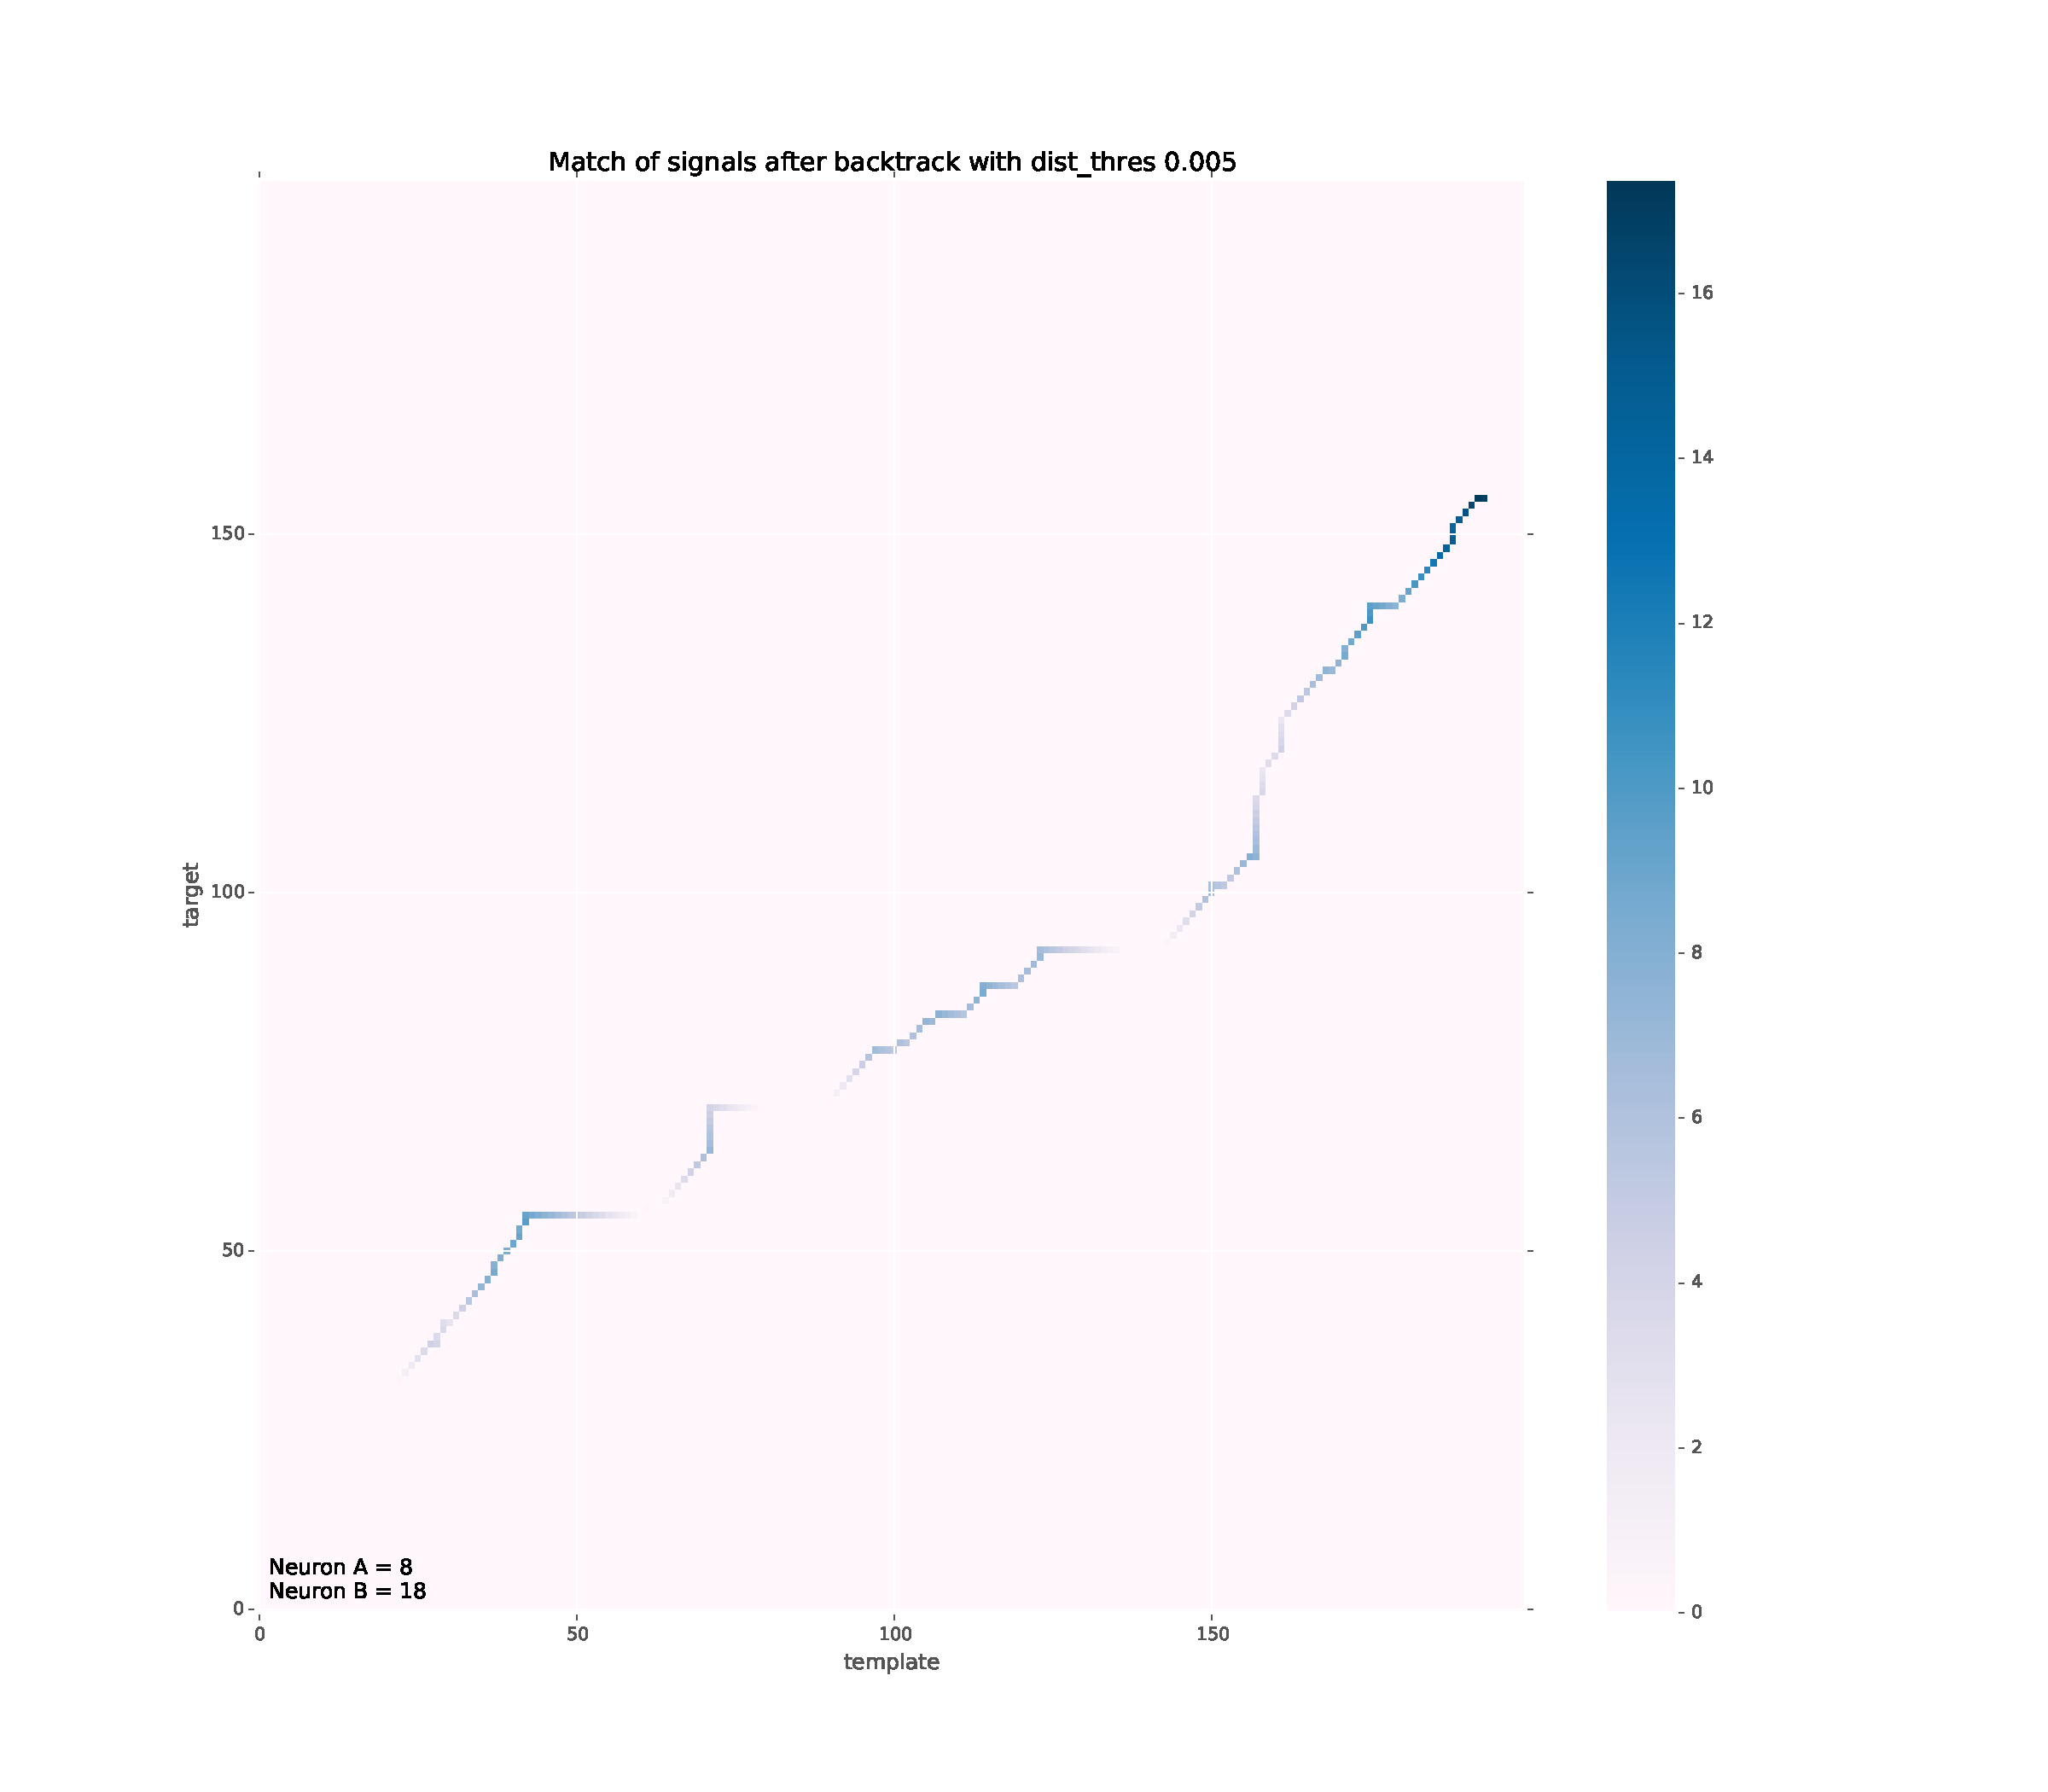
\includegraphics[width=\linewidth]{\plt/apndx/rlcsMain_backtrack_n1_8_n2_182016_05_08_19_30_23.pdf}
    \caption{Score matrix}
  \end{subfigure}%
  \begin{subfigure}[b]{0.5\textwidth}
    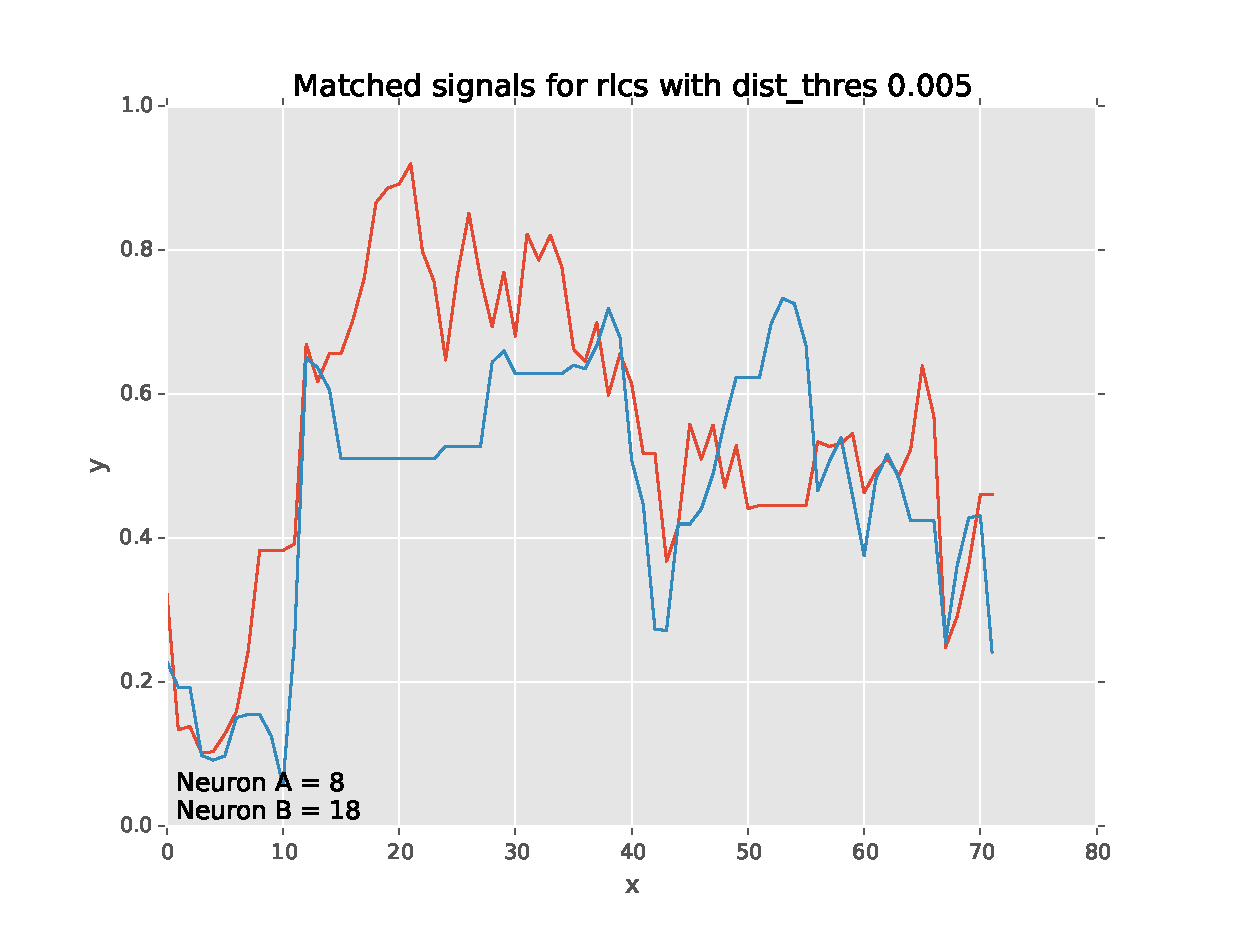
\includegraphics[width=\linewidth]{\plt/apndx/rlcsMain_getSegs_8_n2_182016_05_08_19_30_23}
    \caption{Extracted longest motif}
  \end{subfigure}%
  \caption{RLCS performed on responses of two neurons within a mouse. The two signals have a pearson correlation of 0.02}
  \label{fig:}
\end{figure}
% section rlcs_of_responses_from_two_neurons_in_a_mouse (end)
\FloatBarrier
\section{RLCS of neuronal responses from two different mice} % (fold)
\label{sec:rlcs_of_neuronal_responses_from_two_different_mice}
\begin{figure}[h]
  \begin{subfigure}[b]{0.5\textwidth}
    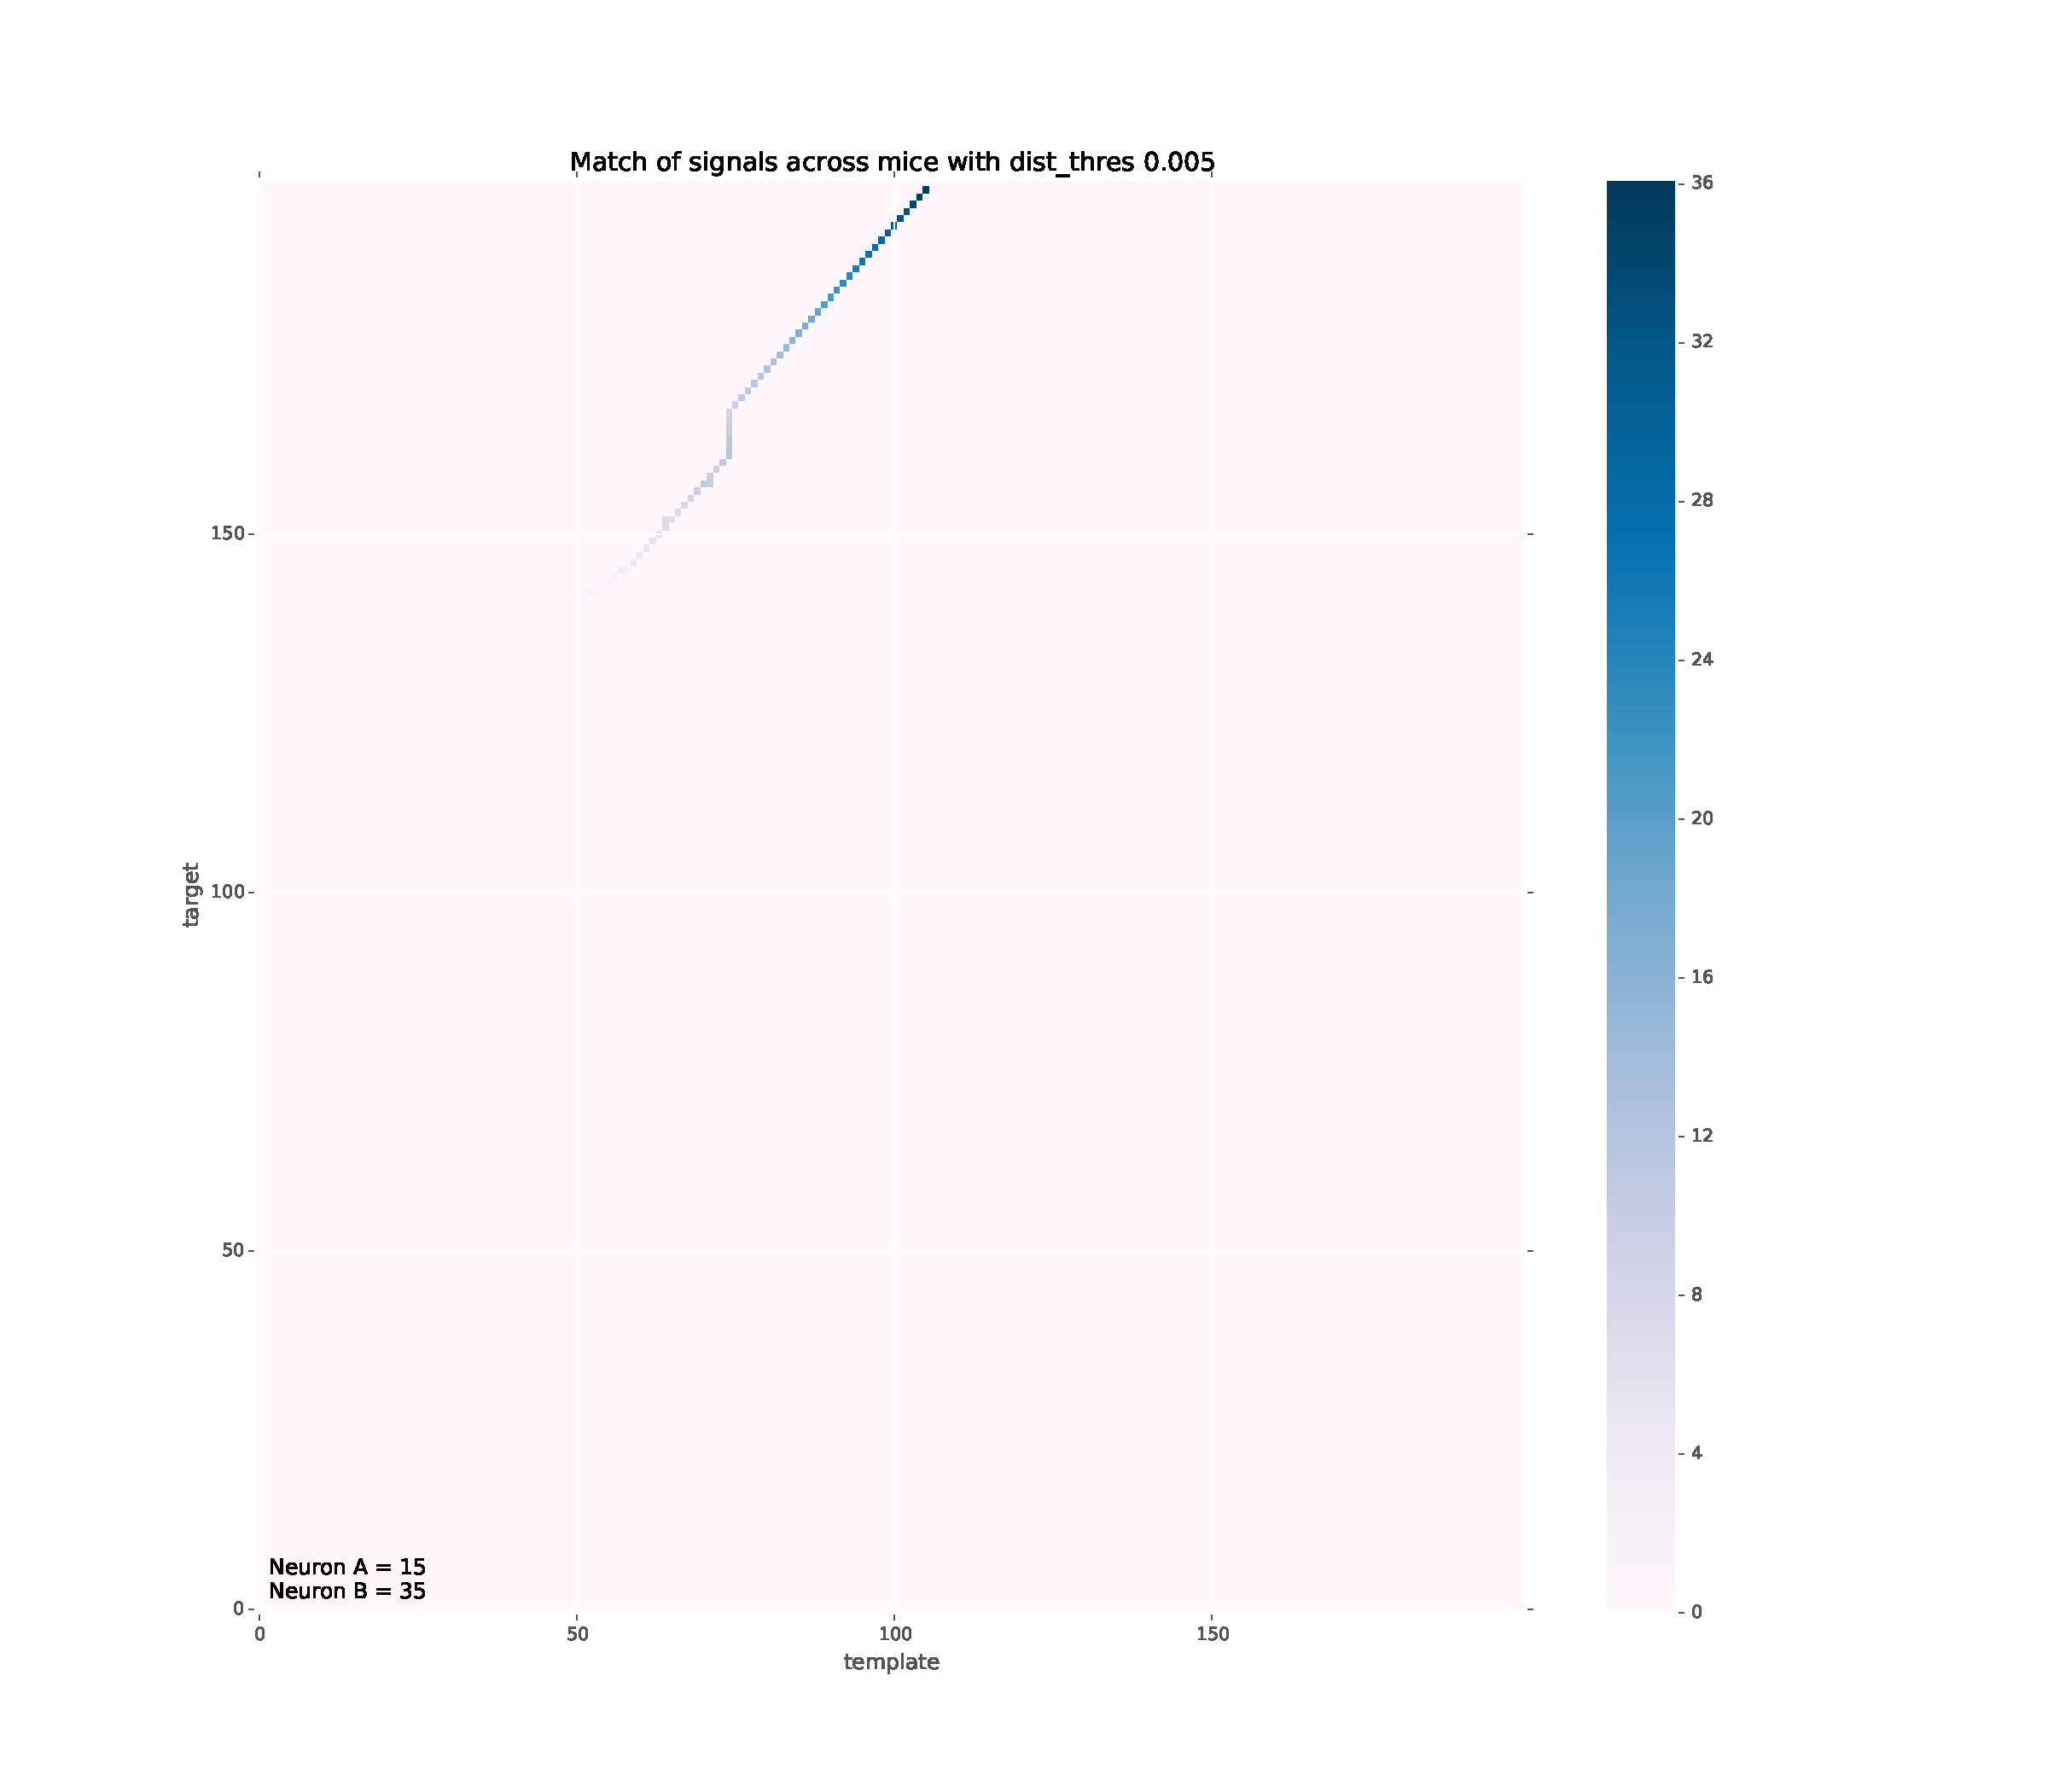
\includegraphics[width=\linewidth]{\plt/apndx/rlcsMain_backtrack_mice_2016_05_08_19_51_44.pdf}
    \caption{Score matrix}
  \end{subfigure}%
  \begin{subfigure}[b]{0.5\textwidth}
    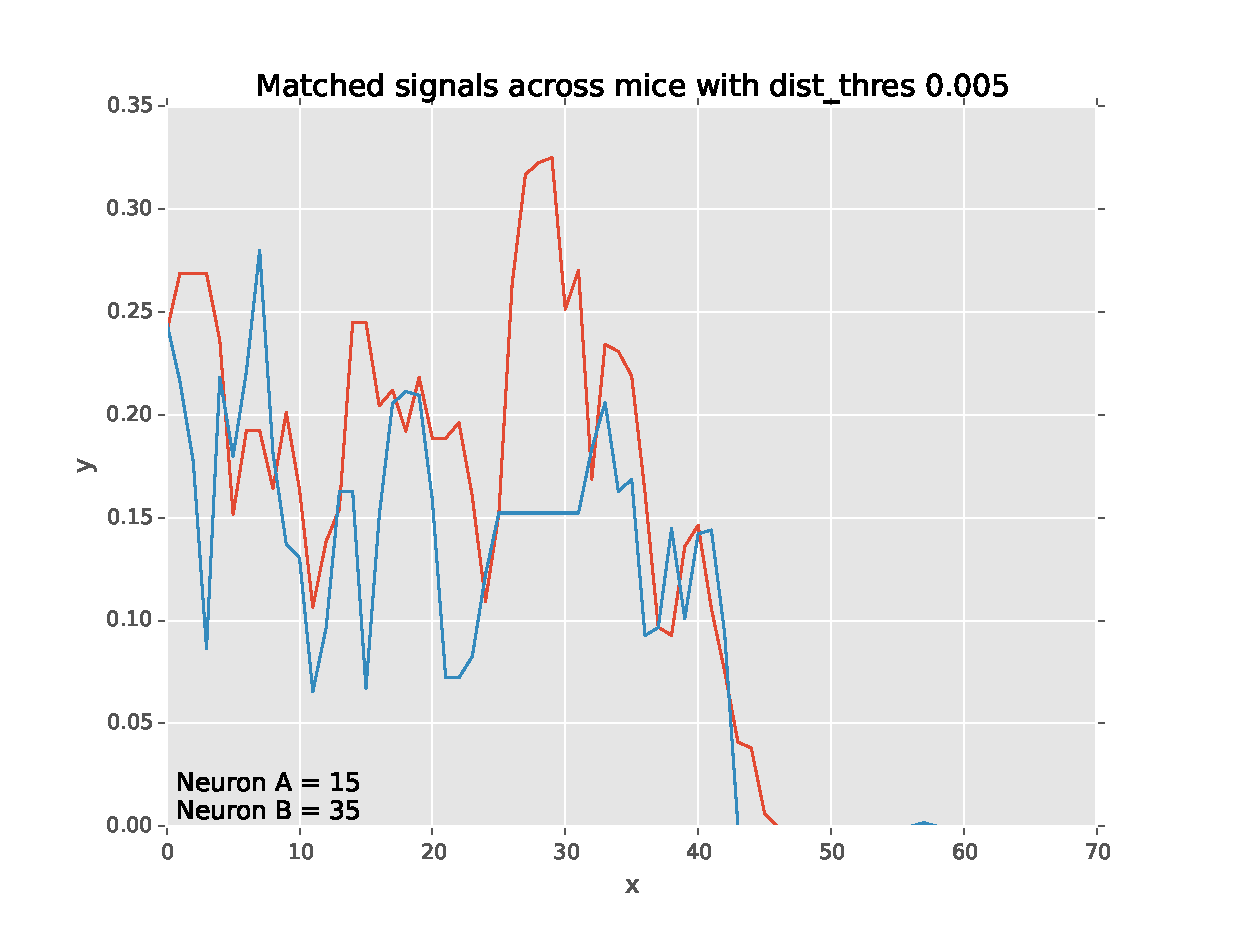
\includegraphics[width=\linewidth]{\plt/apndx/rlcsMain_getSegs_mice2016_05_08_19_51_44}
    \caption{Extracted longest motif}
  \end{subfigure}%
  \caption{RLCS performed on responses of two neurons from different mouse. Note that length of subsequence is smaller than other in cases.}
  \label{fig:}
\end{figure}

\begin{figure}[h]
  \begin{subfigure}[b]{0.5\textwidth}
    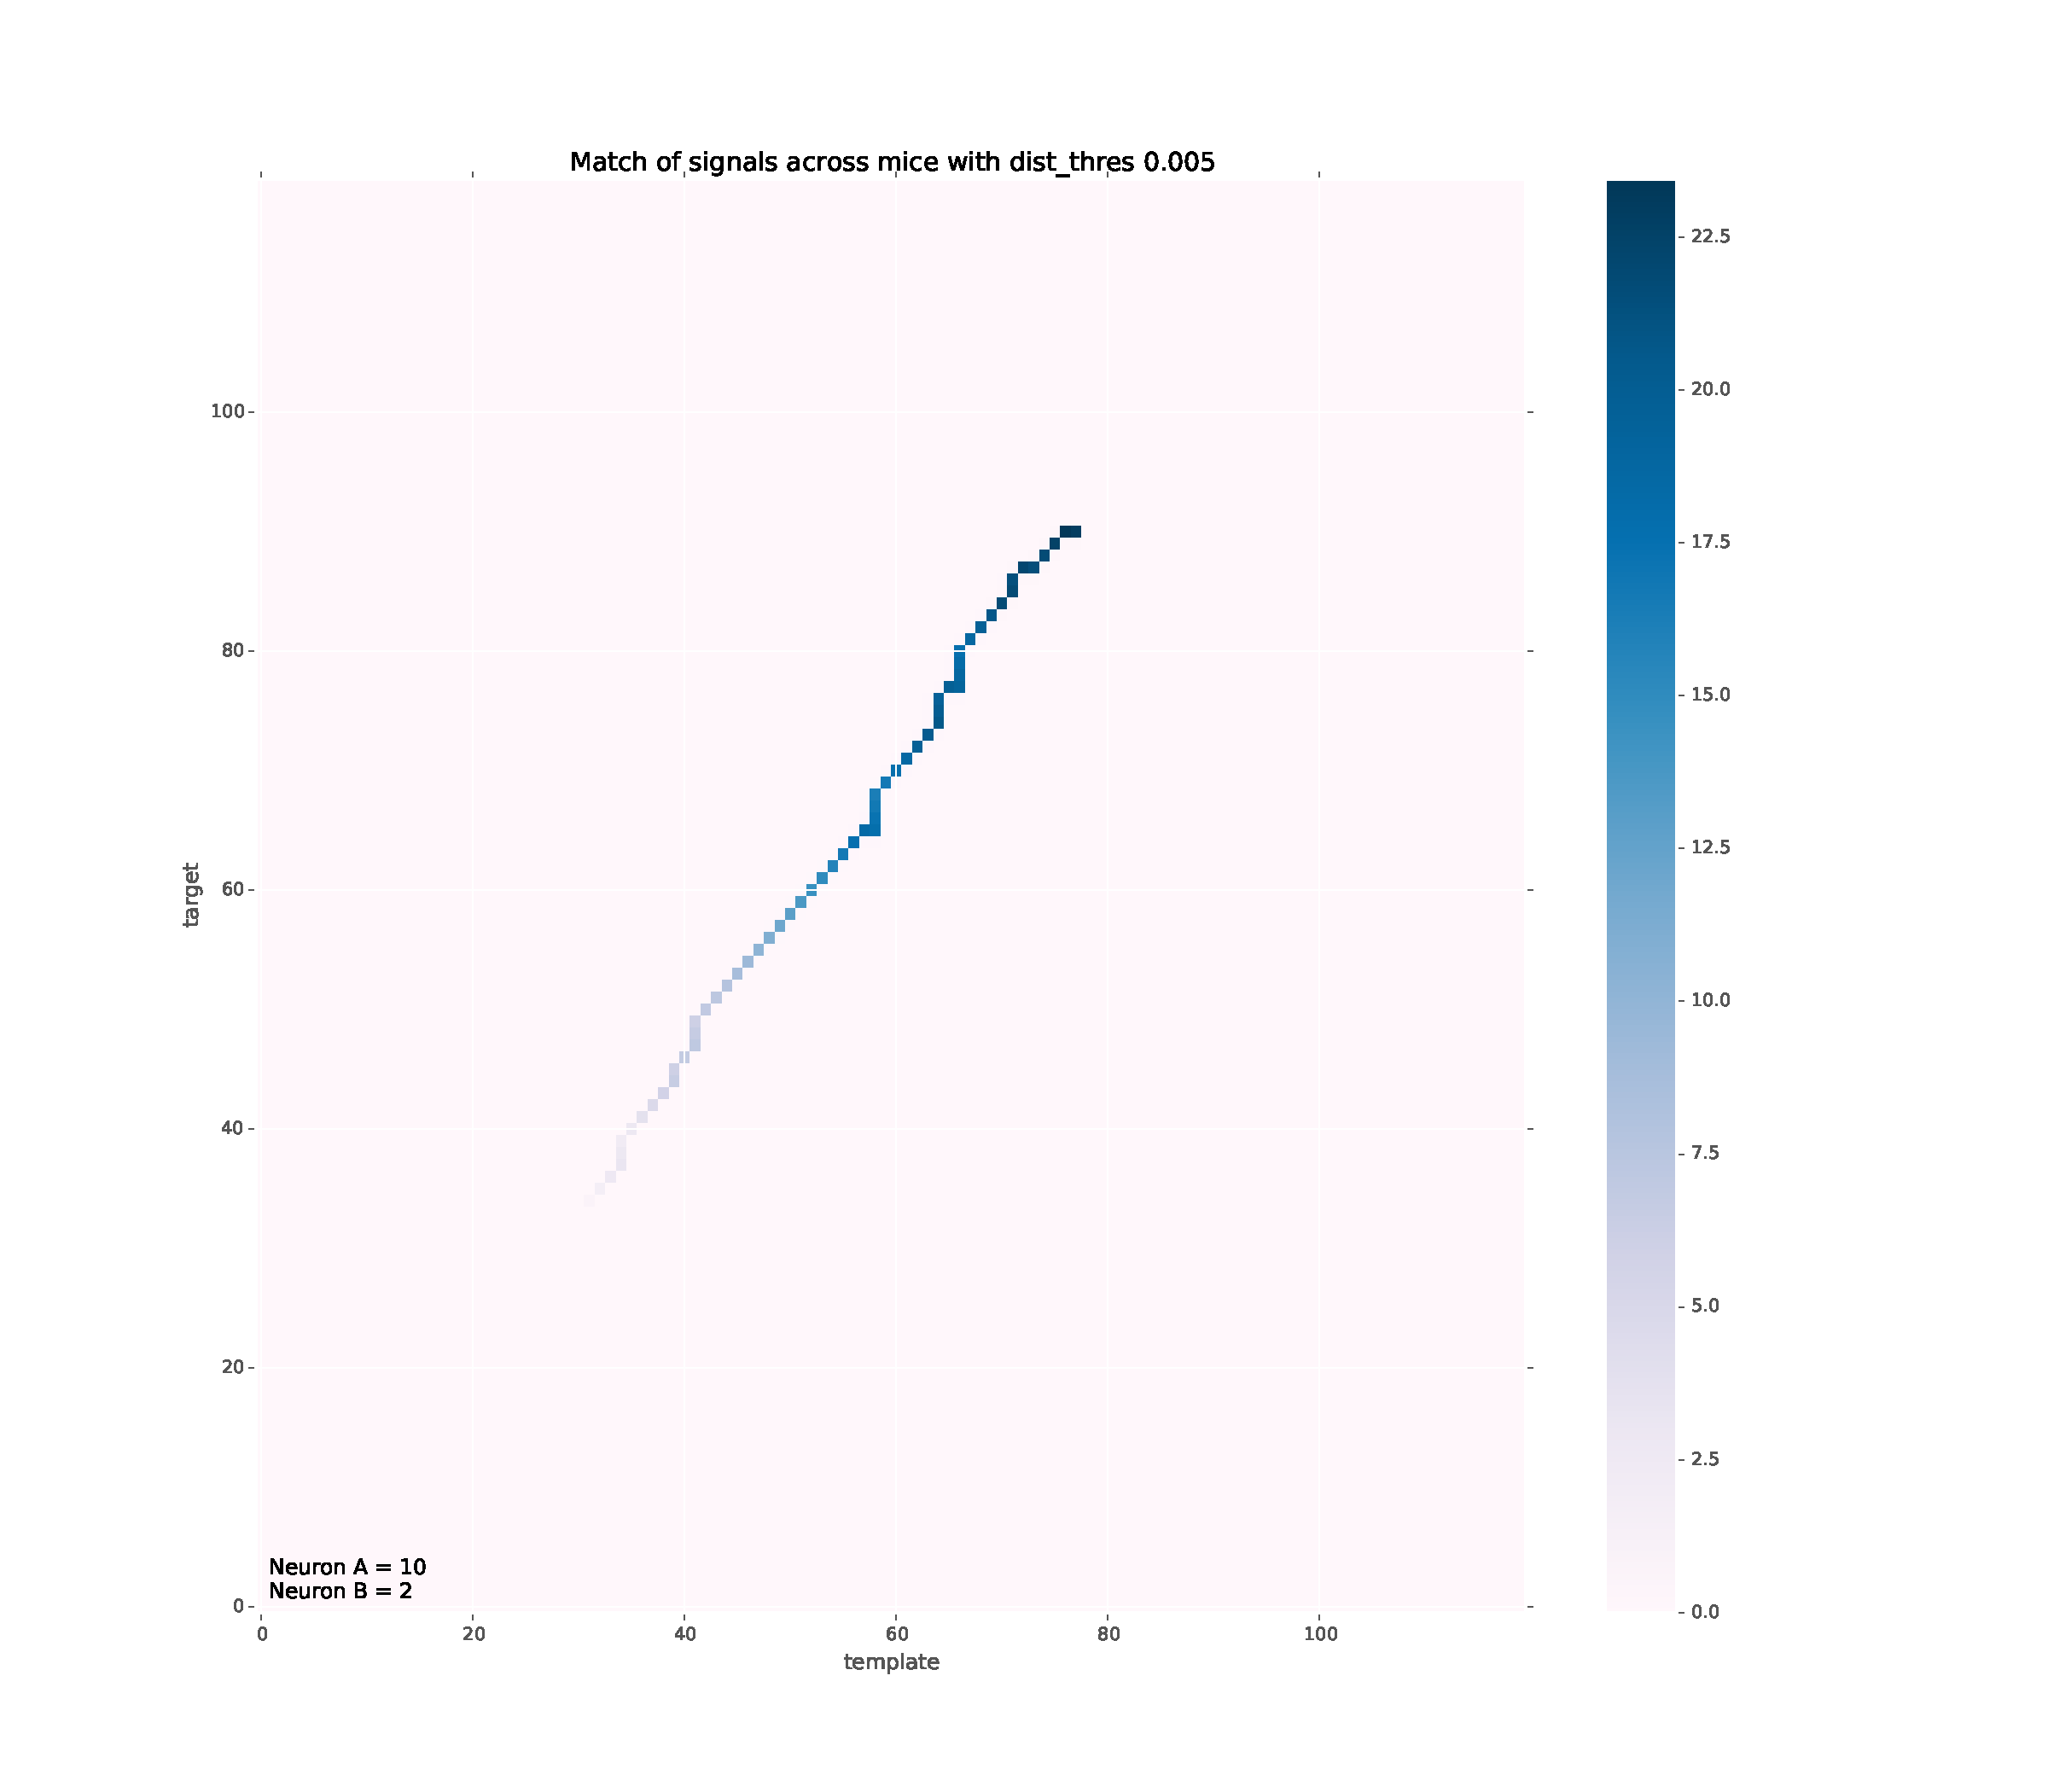
\includegraphics[width=\linewidth]{\plt/apndx/rlcsMain_backtrack_mice_2016_05_08_19_48_28.pdf}
    \caption{Score matrix}
  \end{subfigure}%
  \begin{subfigure}[b]{0.5\textwidth}
    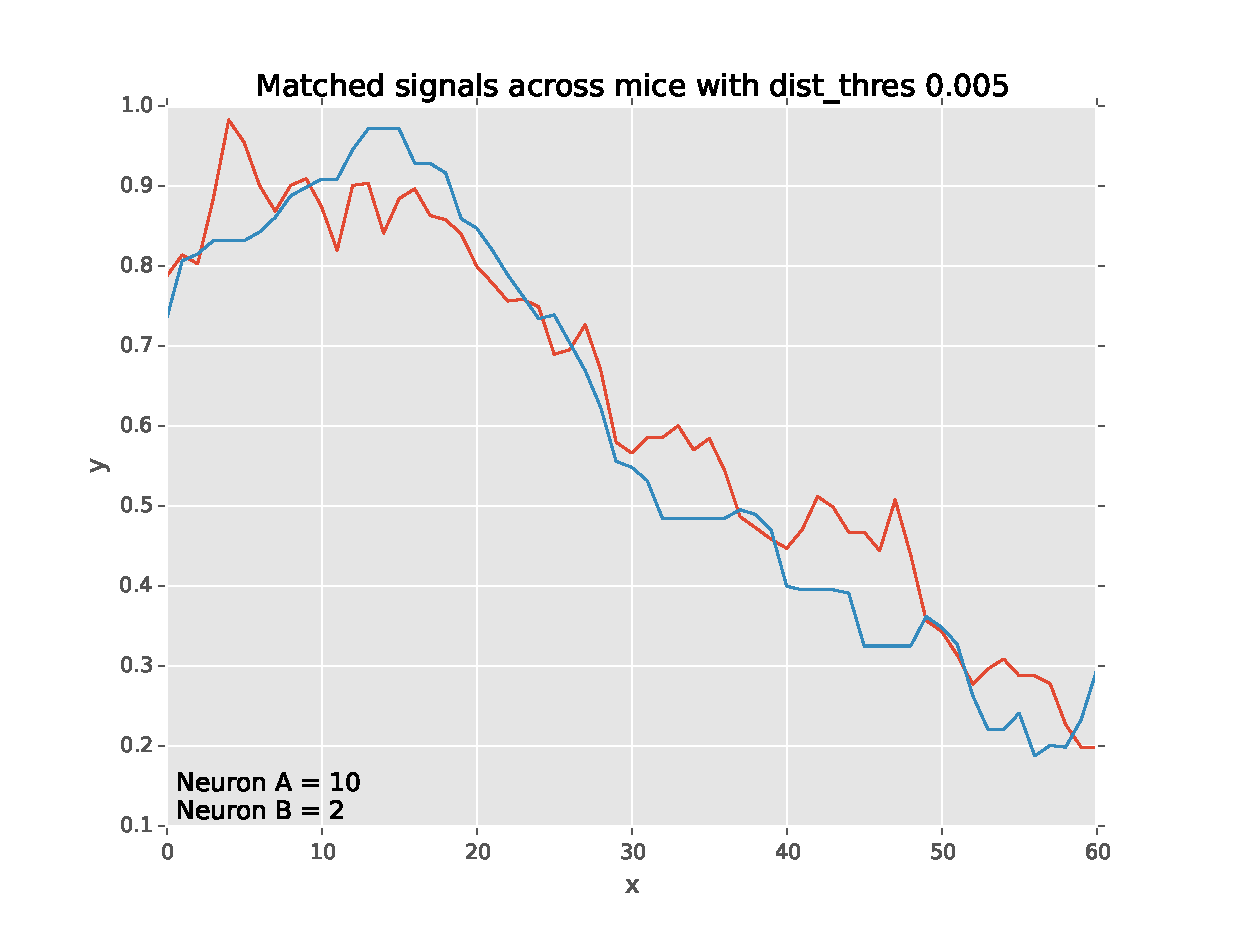
\includegraphics[width=\linewidth]{\plt/apndx/rlcsMain_getSegs_mice2016_05_08_19_48_28}
    \caption{Extracted longest motif}
  \end{subfigure}%
  \caption{RLCS performed on responses of two neurons from different mouse. This motif \textit{across mice} last for 3 seconds. (This data is from drifting sinusoidal grating experiment, in which sample rate is 20Hz)}
  \label{fig:}
\end{figure}

\begin{figure}[h]
  \begin{subfigure}[b]{0.5\textwidth}
    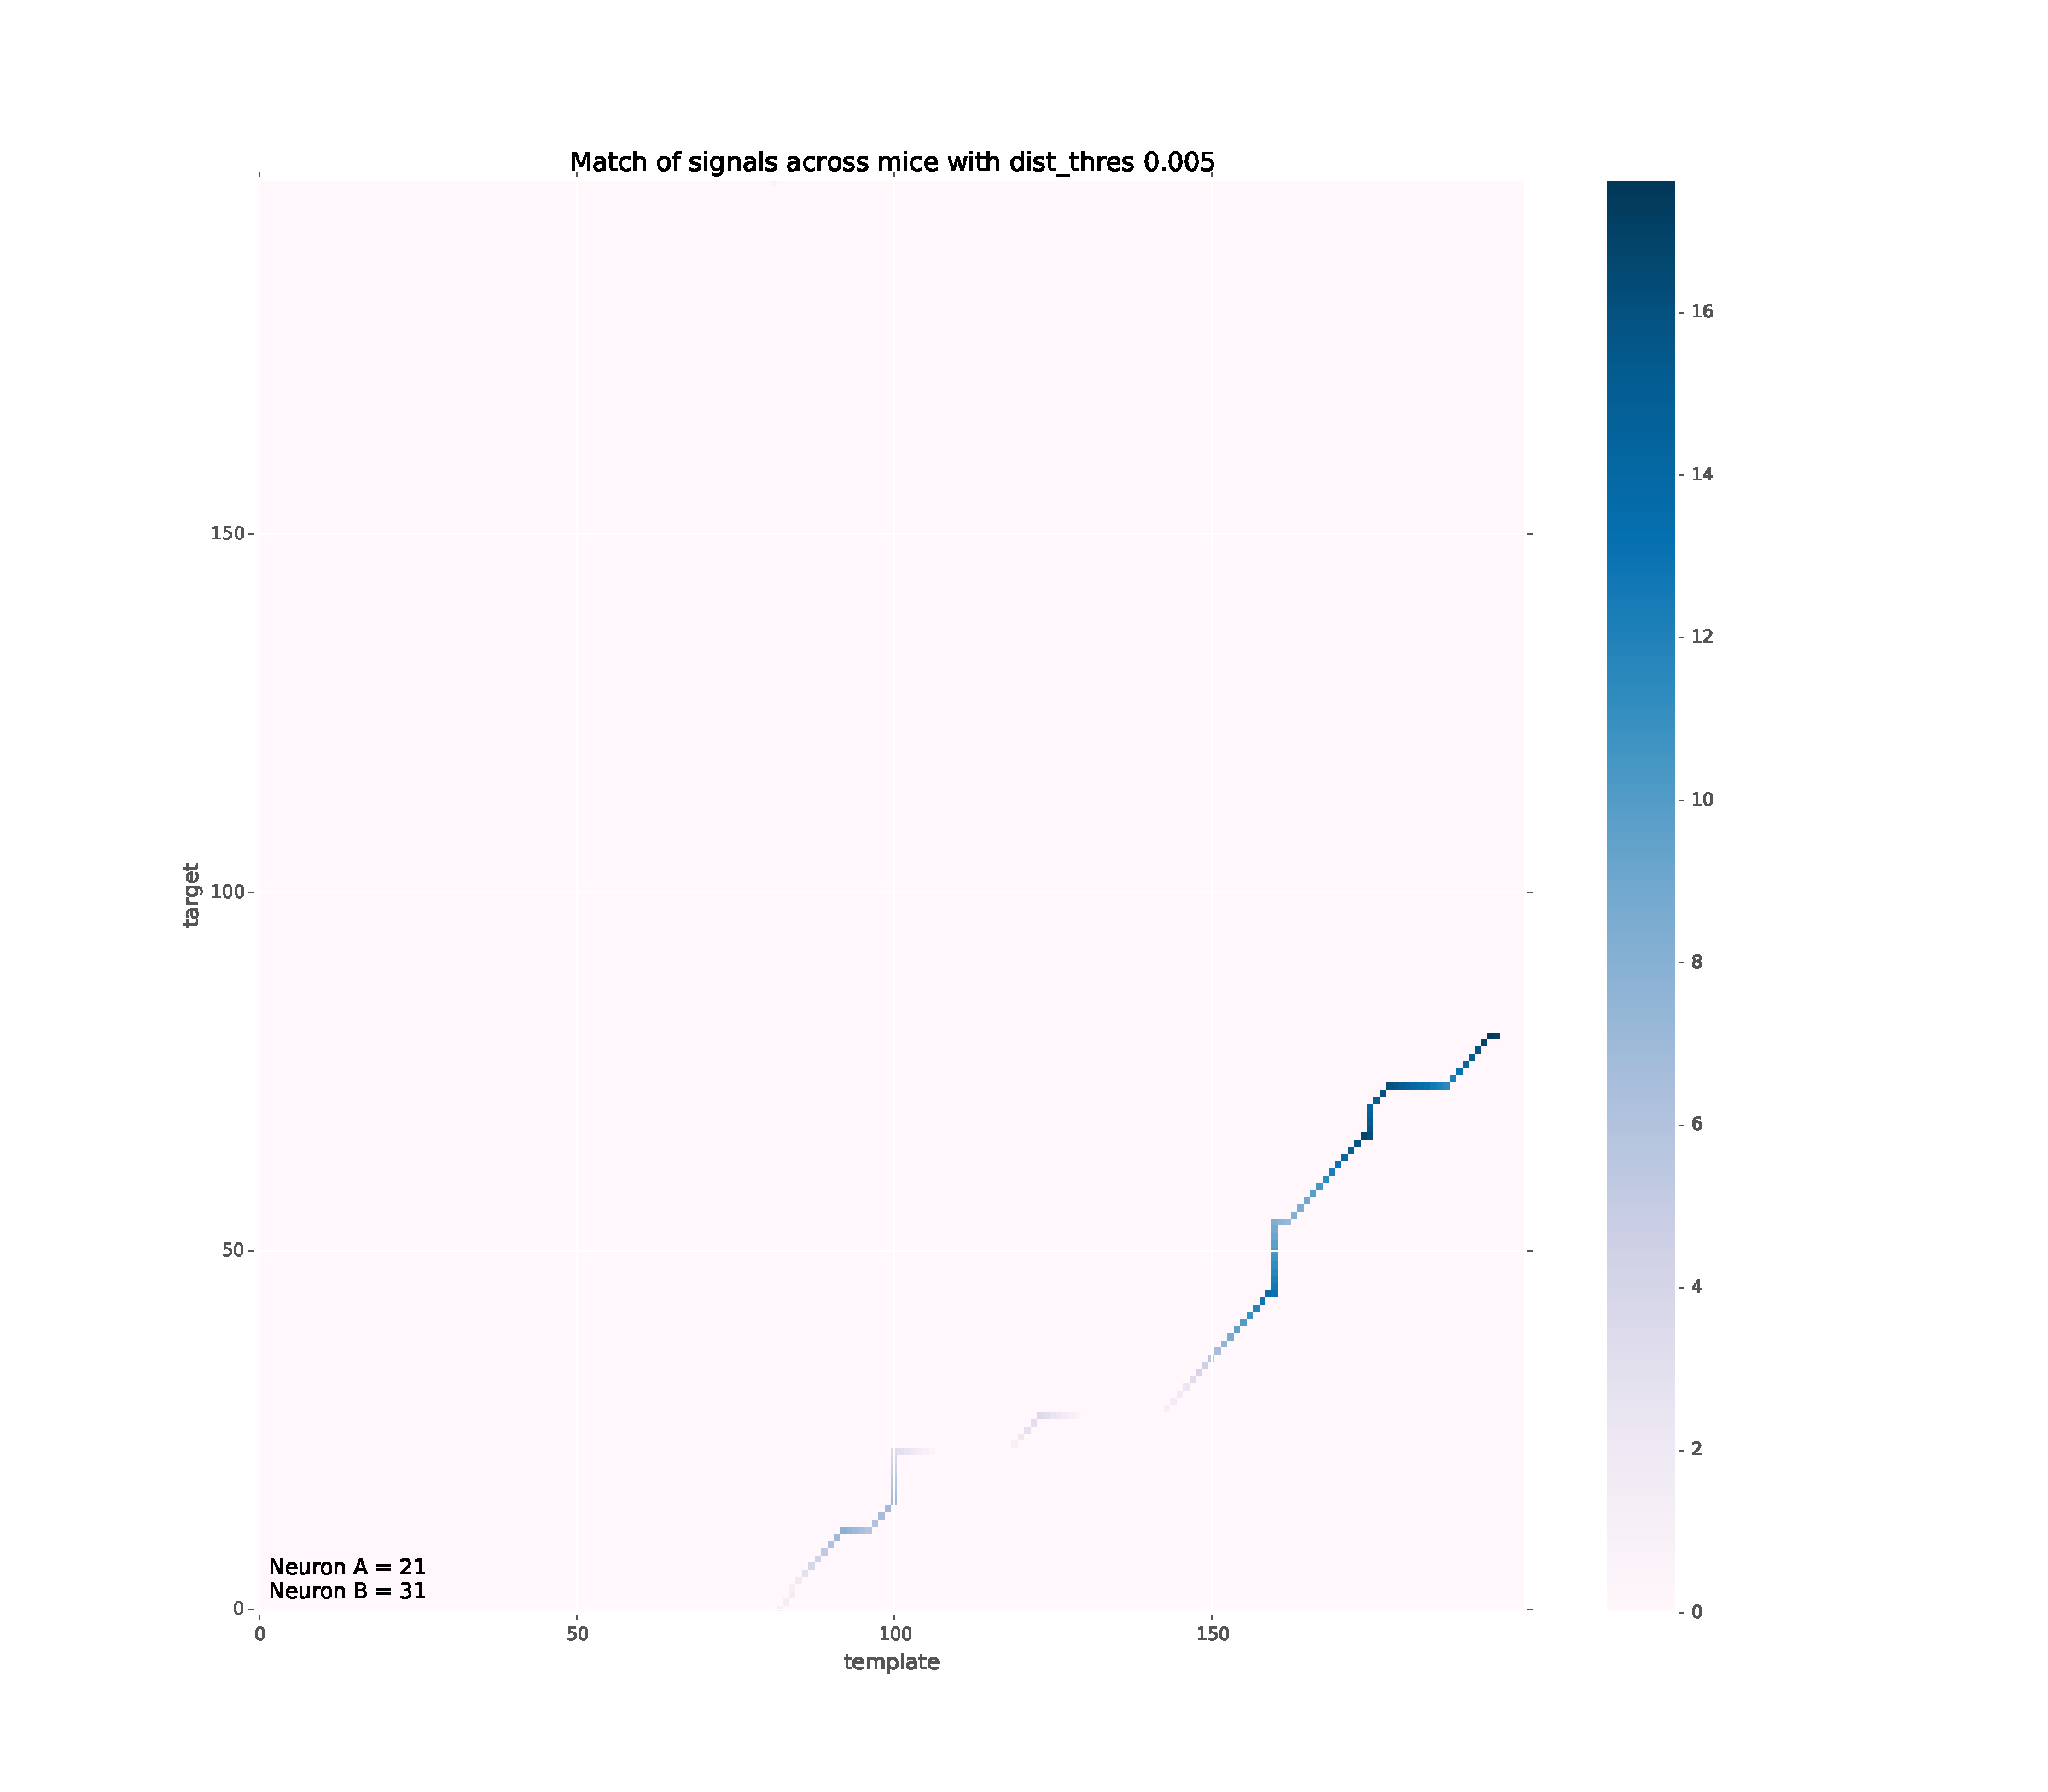
\includegraphics[width=\linewidth]{\plt/apndx/rlcsMain_backtrack_mice_2016_05_08_19_52_57.pdf}
    \caption{Score matrix}
  \end{subfigure}%
  \begin{subfigure}[b]{0.5\textwidth}
    \includegraphics[width=\linewidth]{\plt/apndx/rlcsMain_getSegs_mice2016_05_08_19_52_57}
    \caption{Extracted longest motif}
  \end{subfigure}%
  \caption{RLCS performed on responses of two neurons from different mouse. Note that length of subsequence is smaller than other in cases.}
  \label{fig:}
\end{figure}
% section rlcs_of_neuronal_responses_from_two_different_mice (end)
%%%%%%%%%%%%%%%%%%%%%%%%%%%%%%%%%%%%%%%%%%%%%%%%%%%%%%%%%%%%%%%%%%%%%%
% Bibliography.
\pagebreak
\begin{singlespace}
  \begin{small}
	\bibliography{refs}
  \end{small}
\end{singlespace}
%%%%%%%%%%%%%%%%%%%%%%%%%%%%%%%%%%%%%%%%%%%%%%%%%%%%%%%%%%%%%%%%%%%%%%
\end{document}
